\chapter{Additional material for the Higgs to invisible analysis}
\label{app:supplementary_hinv_plots}

\initial{T}o avoid detracting too much from the predominant results in Chpt.~\ref{chap:higgstoinv}, some figures were omitted from the main text. Apps.~\ref{sec:pre_post_fit_plots_ttH_CRs} and \ref{sec:pre_post_fit_plots_VH_CRs} illustrate the distributions from the \gls{CR}-only fit for \ttH and \VH channels, respectively. Each category and \ptmiss bin is shown for each data taking period in Run-2. While the yields for individual backgrounds are post-fit, the total pre-fit \acrshort{mc} is also displayed for comparisons to data as well as the post-fit prediction. Event counts in the signal region from the \gls{CR}-only fit are tabulated in App.~\ref{sec:yield_tables_SR_CR_only_fit}. One table is provided per data taking year. Each table is contains the yields of the data and total \acrshort{sm} background (with further columns decomposing the latter into its components) in every category and \ptmiss bin. The rate parameters from the \gls{CR}-only fits, with \acrshort{mc}, data, and the predicted background yields in the signal region are tabulated in App.~\ref{sec:rate_params_CR_only_fit}.

Apps.~\ref{sec:B_only_fit_plots_ttH_SR} and \ref{sec:B_only_fit_plots_VH_SR} comprise the distributions in the signal region from the background-only fit. Event counts are presented in App.~\ref{sec:yield_tables_SR_B_only_fit}.

App.~\ref{sec:limits_likelihoods_cats_supplementary} includes limit plots broken down by category and data taking period for each of the analysis categories.


%=========================================================


\section{Control region-only fits to the \texorpdfstring{\ttH}{ttH} categories}
\label{sec:pre_post_fit_plots_ttH_CRs}

\begin{figure}[htbp]
    \centering
    \begin{subfigure}[b]{0.65\textwidth}
        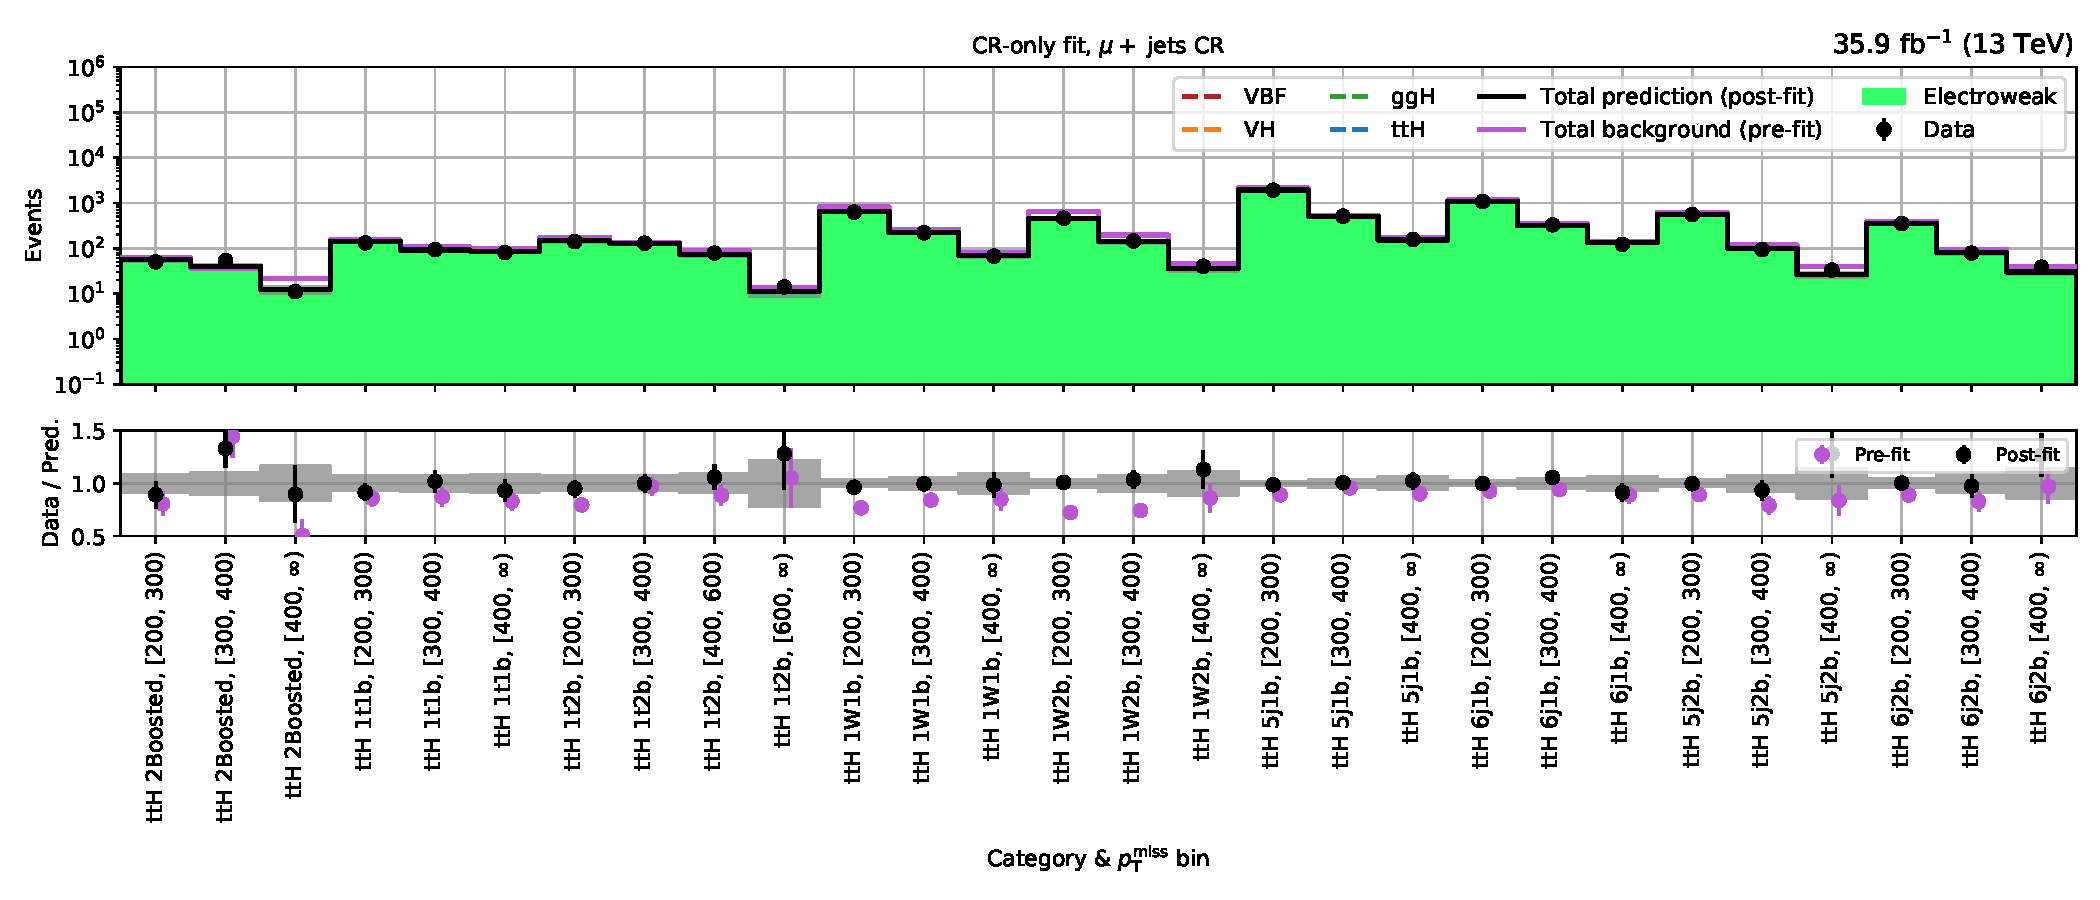
\includegraphics[width=\textwidth]{chapters/higgstoinv/figures/mountain_ranges/2016/ttH/Wmunu_tree_fit_b-abs_values_ttH_cats.pdf}
        \caption{\ttH --- \singleMuCr \gls{CR} (2016)}
    \end{subfigure}

    \begin{subfigure}[b]{0.65\textwidth}
        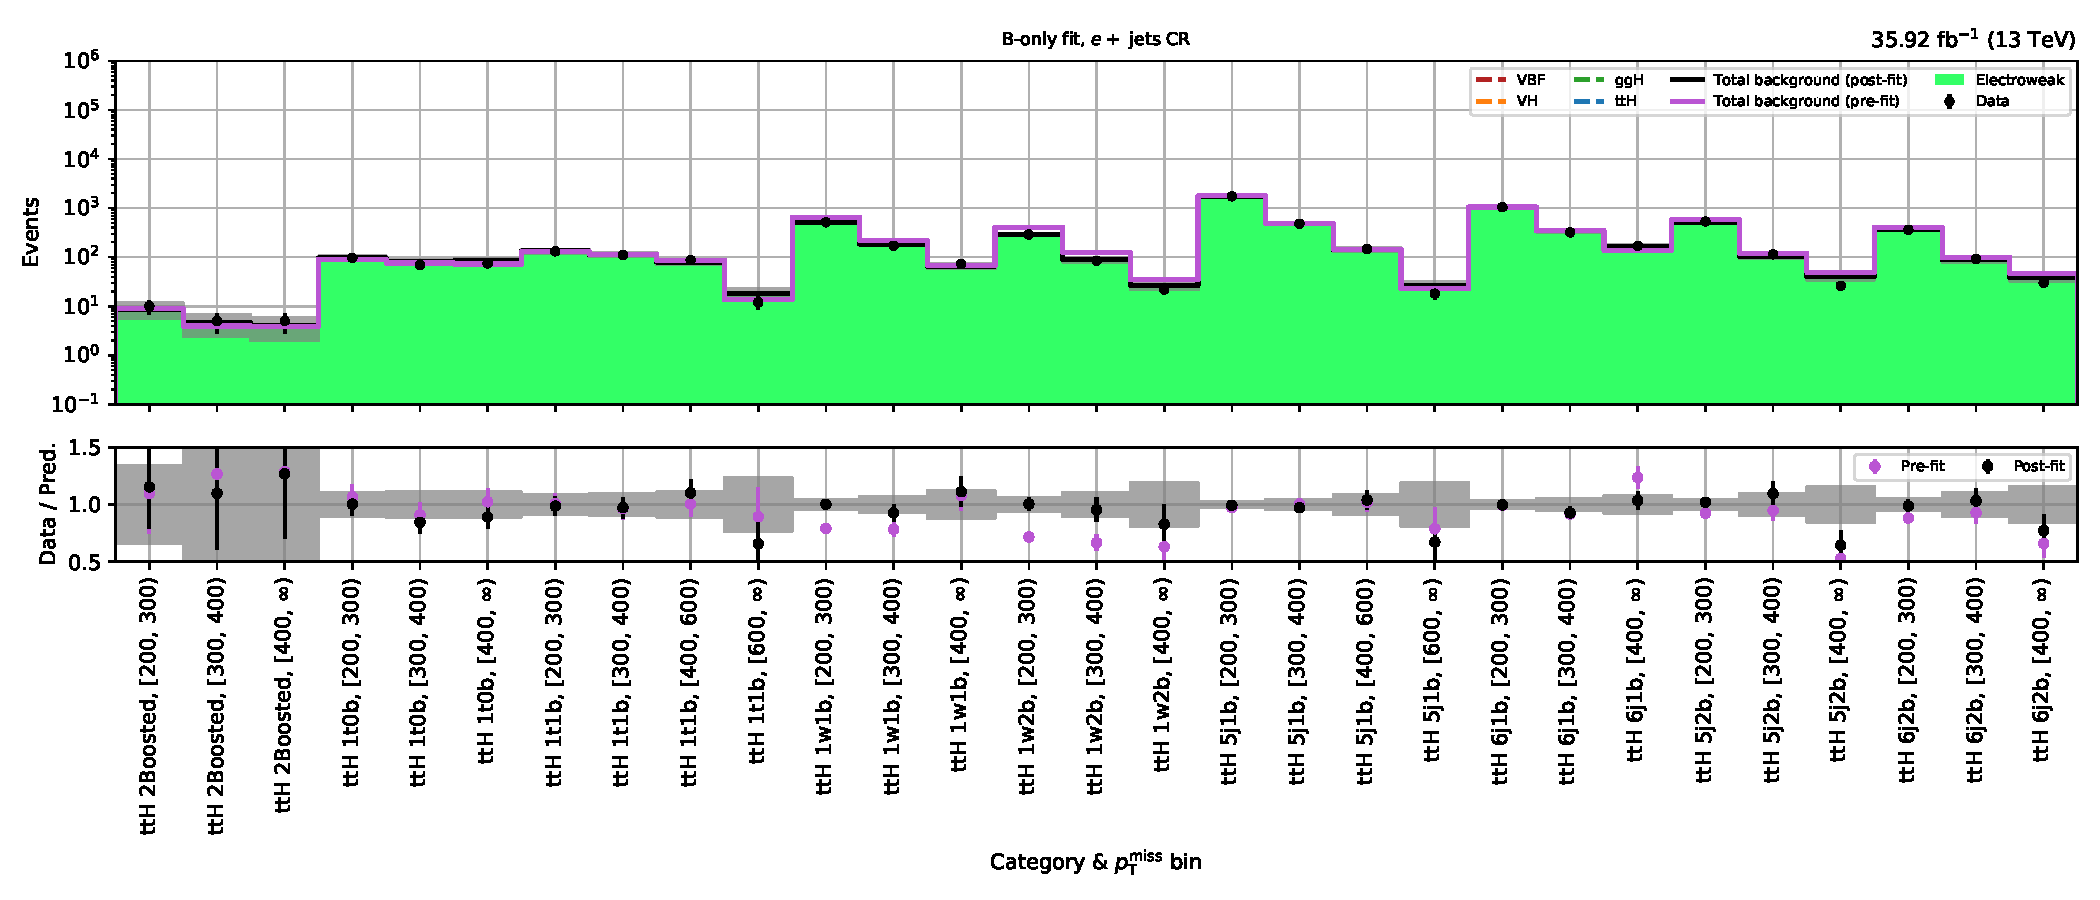
\includegraphics[width=\textwidth]{chapters/higgstoinv/figures/mountain_ranges/2016/ttH/Wenu_tree_fit_b-abs_values_ttH_cats.pdf}
        \caption{\ttH --- \singleEleCr \gls{CR} (2016)}
    \end{subfigure}

    \begin{subfigure}[b]{0.65\textwidth}
        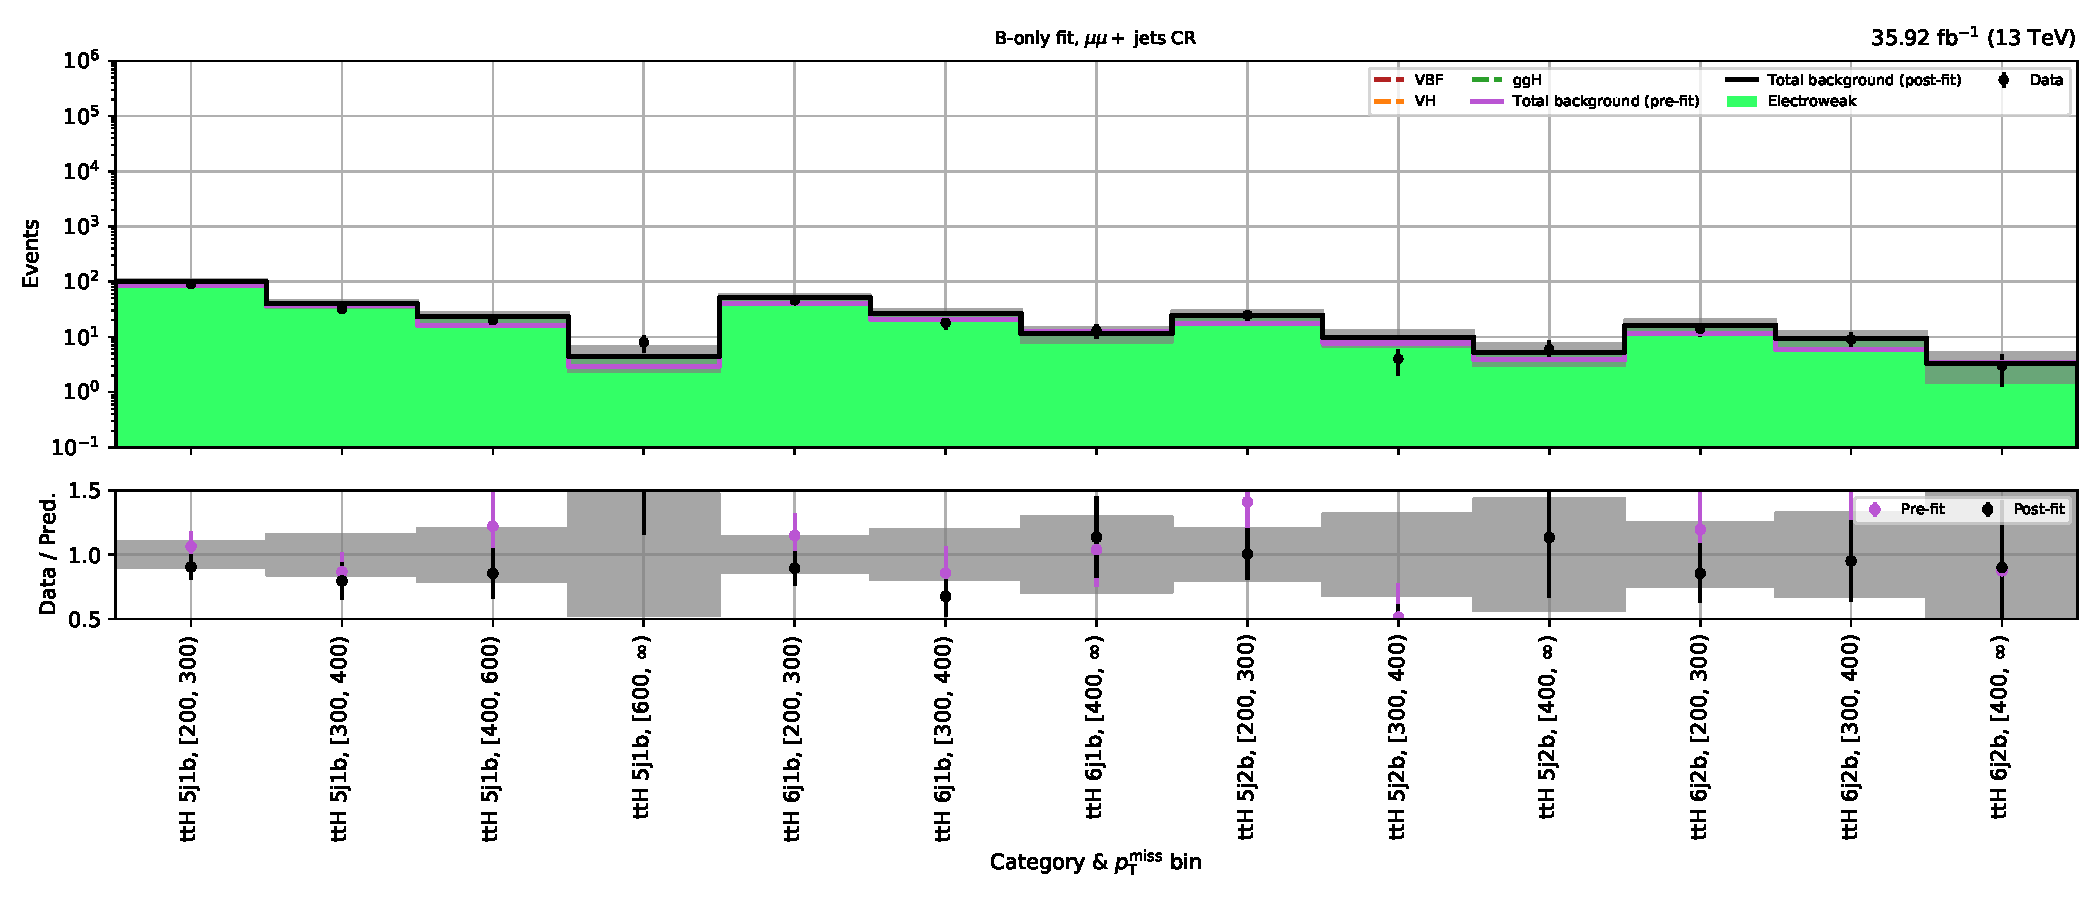
\includegraphics[width=\textwidth]{chapters/higgstoinv/figures/mountain_ranges/2016/ttH/Zmumu_tree_fit_b-abs_values_ttH_cats.pdf}
        \caption{\ttH --- \doubleMuCr \gls{CR} (2016)}
    \end{subfigure}

    \begin{subfigure}[b]{0.65\textwidth}
        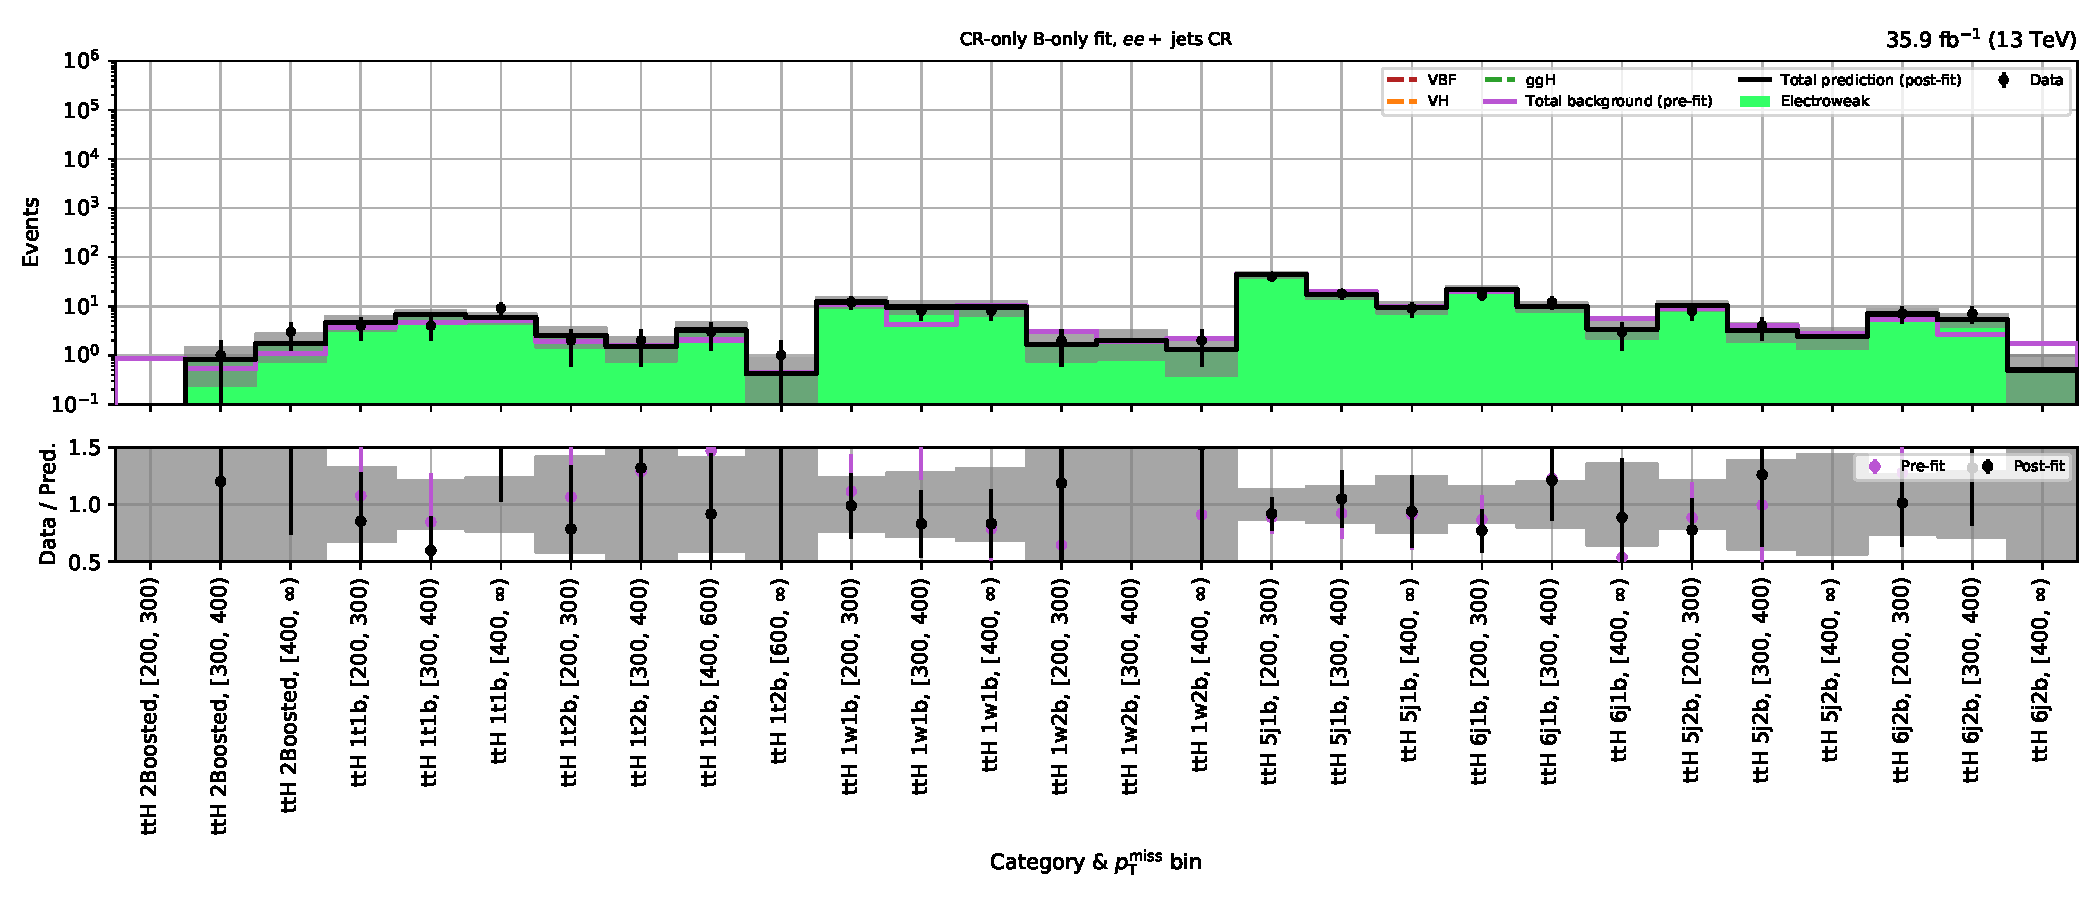
\includegraphics[width=\textwidth]{chapters/higgstoinv/figures/mountain_ranges/2016/ttH/Zee_tree_fit_b-abs_values_ttH_cats.pdf}
        \caption{\ttH --- \doubleEleCr \gls{CR} (2016)}
    \end{subfigure}
    \caption[Post-fit yields for each \ttH category and \ptmiss bin in the lepton control regions for the 2016 dataset]{Post-fit yields for each \ttH category and \ptmiss bin in the lepton \glspl{CR} for the 2016 dataset. The total background pre-fit and post-fit is compared to data in the lower panel of each subfigure.}
    \label{fig:htoinv_mountain_range_ttH_2016_CRs}
\end{figure}

\begin{figure}[htbp]
    \centering
    \begin{subfigure}[b]{0.65\textwidth}
        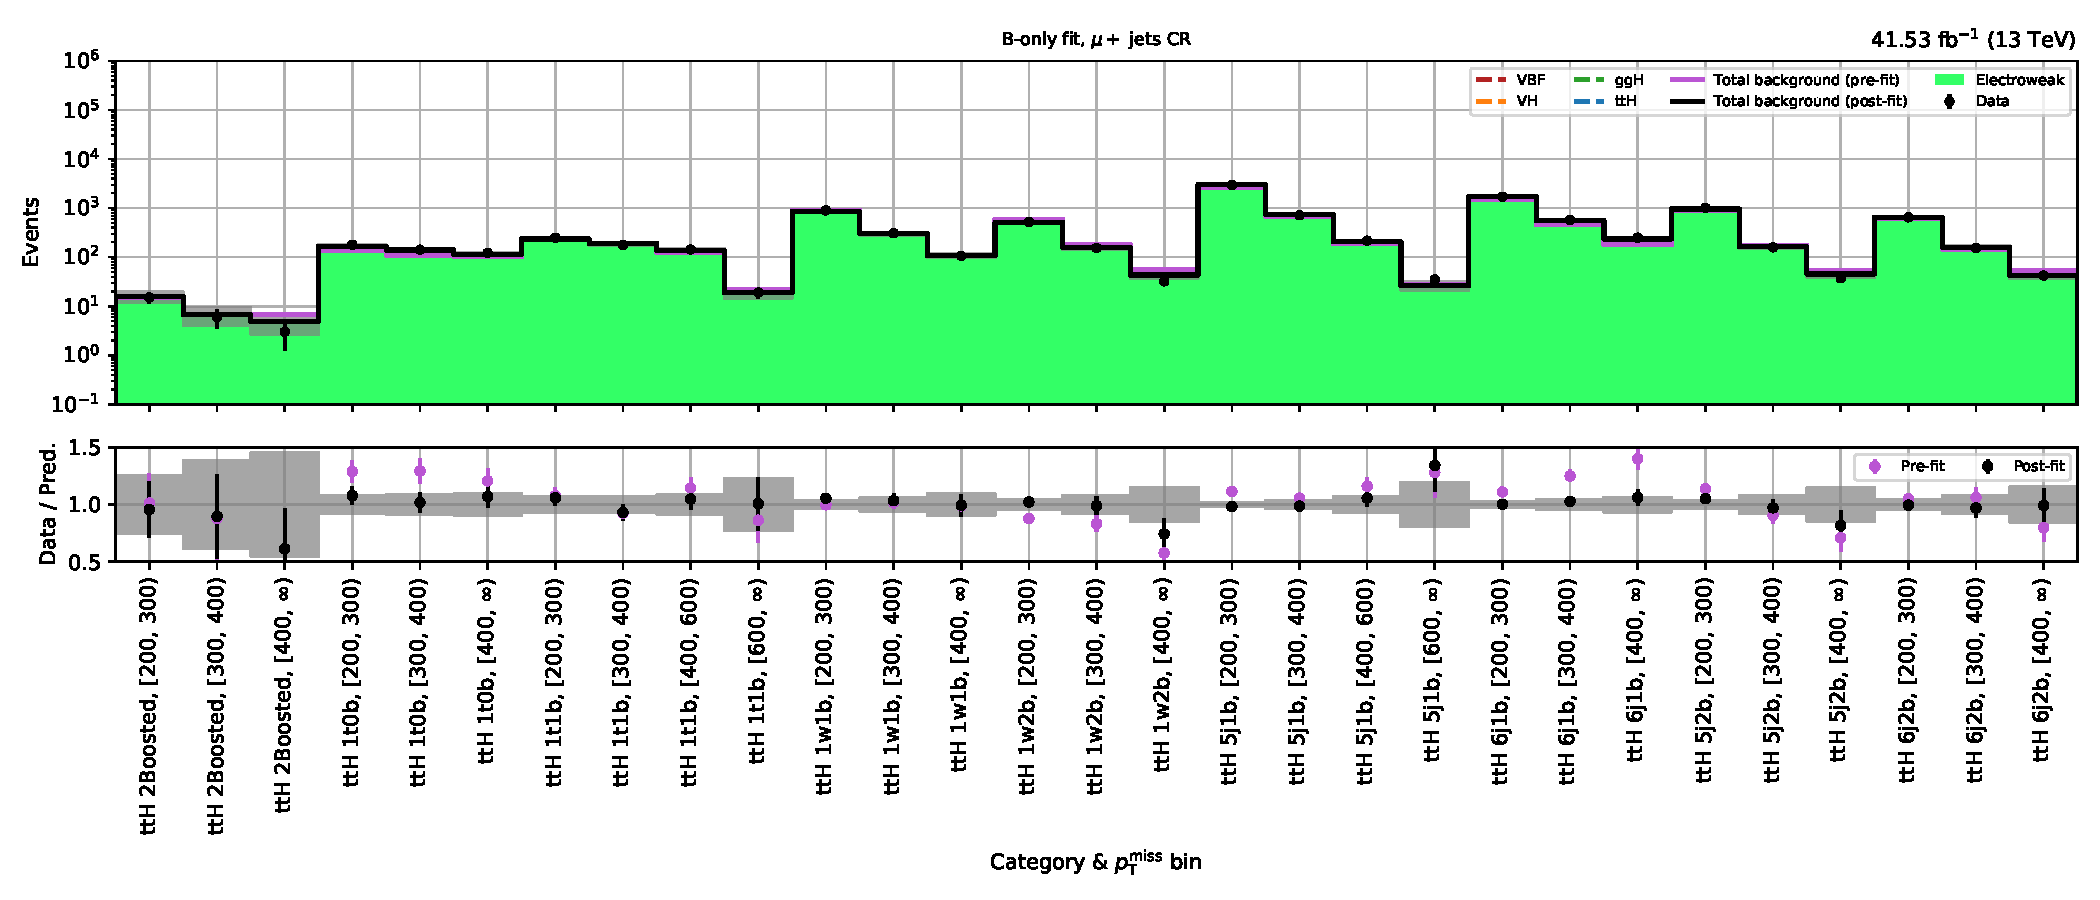
\includegraphics[width=\textwidth]{chapters/higgstoinv/figures/mountain_ranges/2017/ttH/Wmunu_tree_fit_b-abs_values_ttH_cats.pdf}
        \caption{\ttH --- \singleMuCr \gls{CR} (2017)}
    \end{subfigure}

    \begin{subfigure}[b]{0.65\textwidth}
        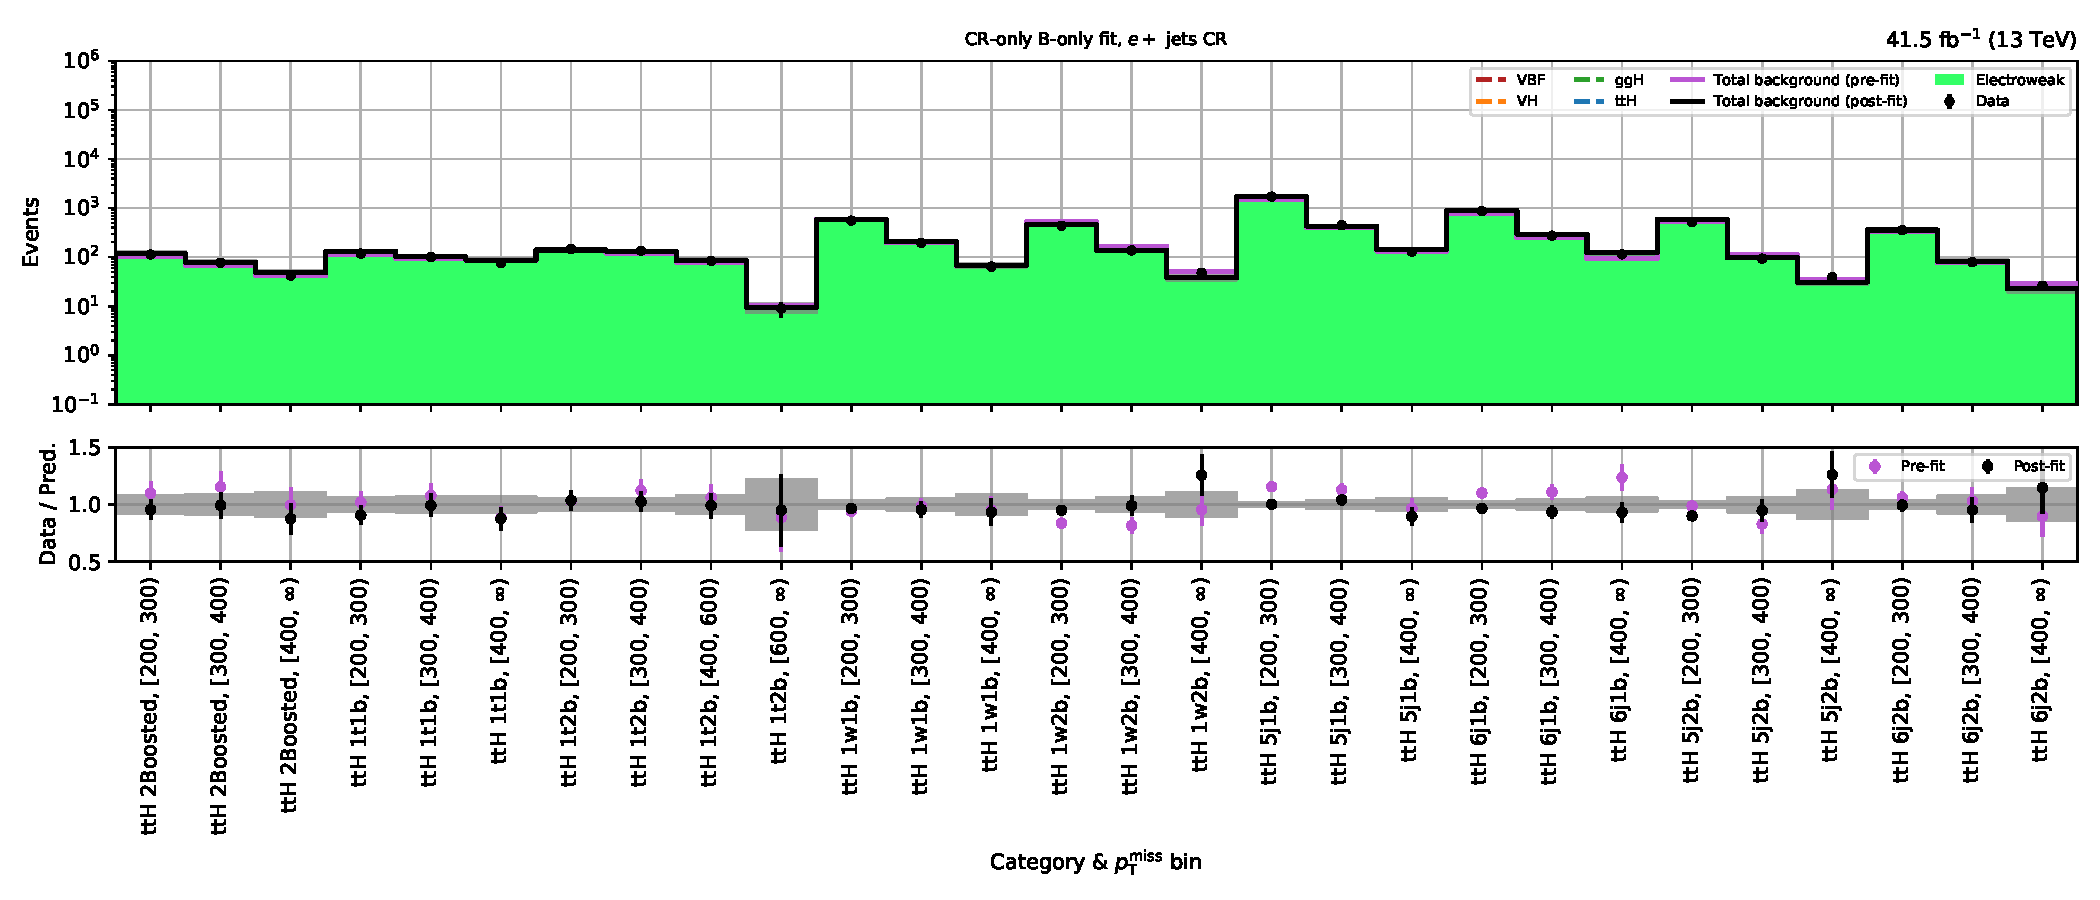
\includegraphics[width=\textwidth]{chapters/higgstoinv/figures/mountain_ranges/2017/ttH/Wenu_tree_fit_b-abs_values_ttH_cats.pdf}
        \caption{\ttH --- \singleEleCr \gls{CR} (2017)}
    \end{subfigure}

    \begin{subfigure}[b]{0.65\textwidth}
        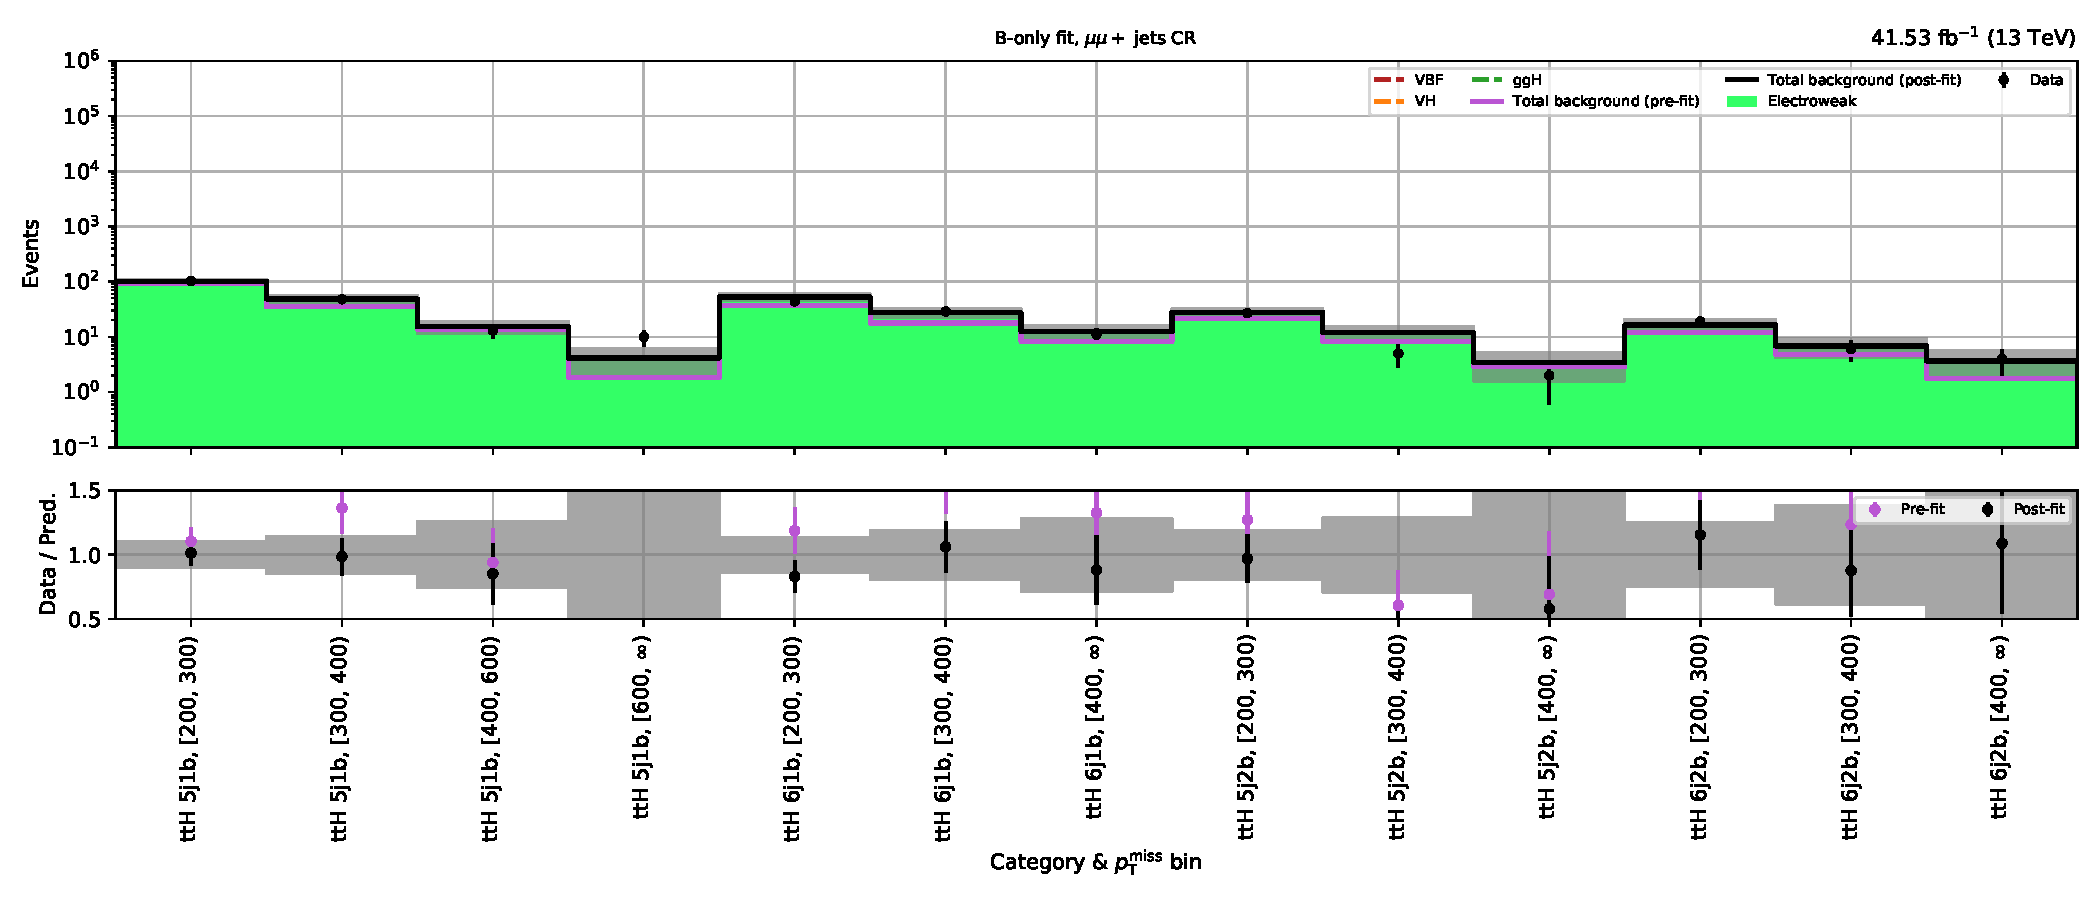
\includegraphics[width=\textwidth]{chapters/higgstoinv/figures/mountain_ranges/2017/ttH/Zmumu_tree_fit_b-abs_values_ttH_cats.pdf}
        \caption{\ttH --- \doubleMuCr \gls{CR} (2017)}
    \end{subfigure}

    \begin{subfigure}[b]{0.65\textwidth}
        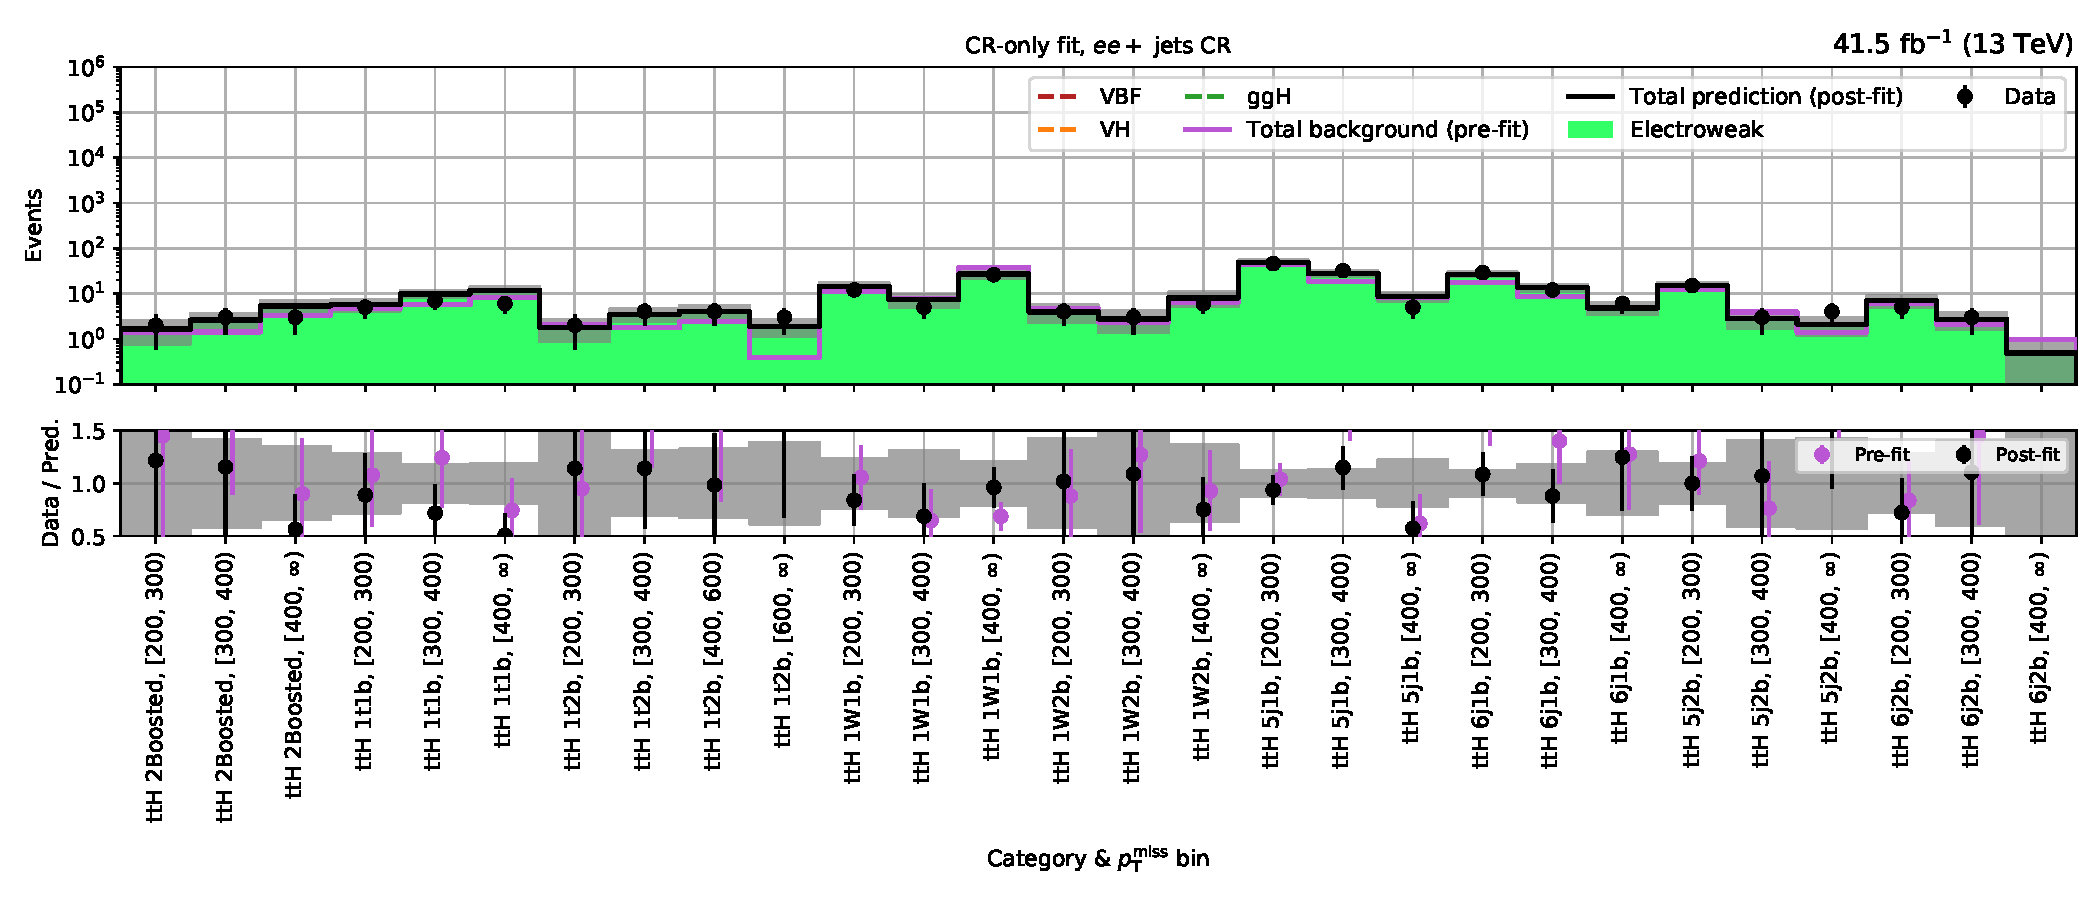
\includegraphics[width=\textwidth]{chapters/higgstoinv/figures/mountain_ranges/2017/ttH/Zee_tree_fit_b-abs_values_ttH_cats.pdf}
        \caption{\ttH --- \doubleEleCr \gls{CR} (2017)}
    \end{subfigure}
    \caption[Post-fit yields for each \ttH category and \ptmiss bin in the lepton control regions for the 2017 dataset]{Post-fit yields for each \ttH category and \ptmiss bin in the lepton \glspl{CR} for the 2017 dataset. The total background pre-fit and post-fit is compared to data in the lower panel of each subfigure.}
    \label{fig:htoinv_mountain_range_ttH_2017_CRs}
\end{figure}

\begin{figure}[htbp]
    \centering
    \begin{subfigure}[b]{0.65\textwidth}
        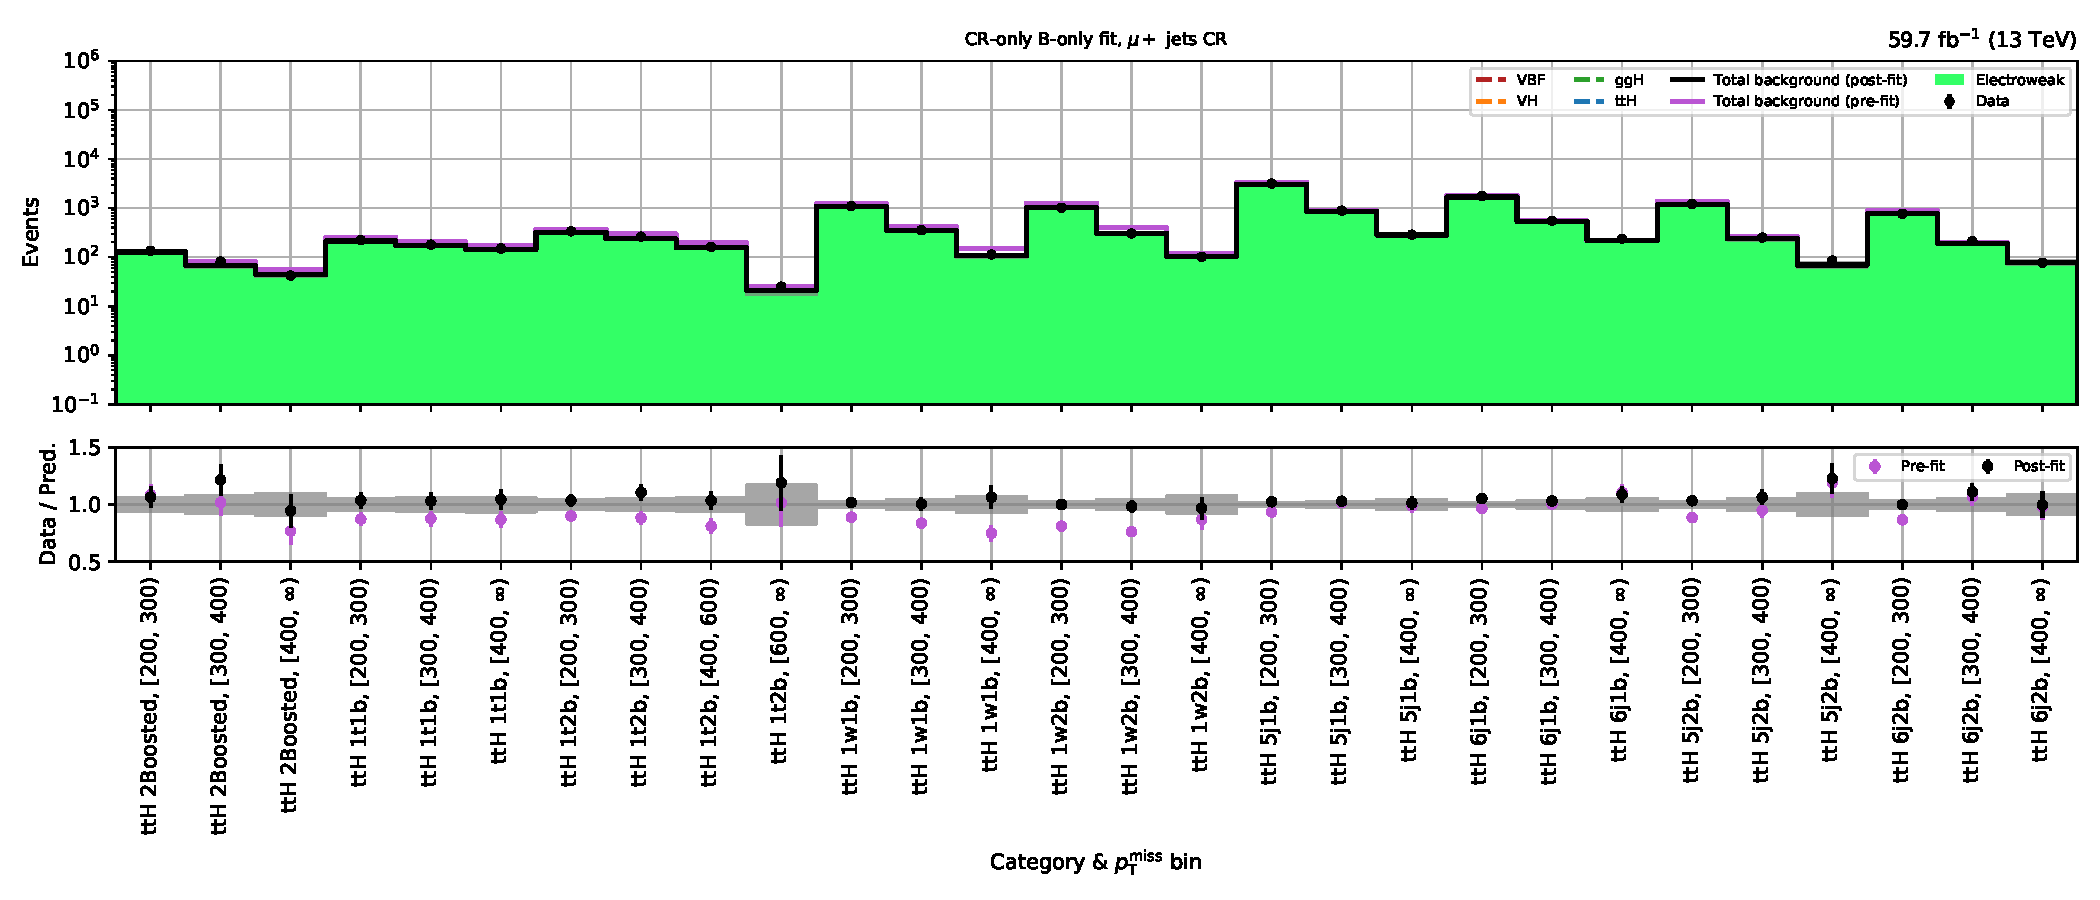
\includegraphics[width=\textwidth]{chapters/higgstoinv/figures/mountain_ranges/2018/ttH/Wmunu_tree_fit_b-abs_values_ttH_cats.pdf}
        \caption{\ttH --- \singleMuCr \gls{CR} (2018)}
    \end{subfigure}

    \begin{subfigure}[b]{0.65\textwidth}
        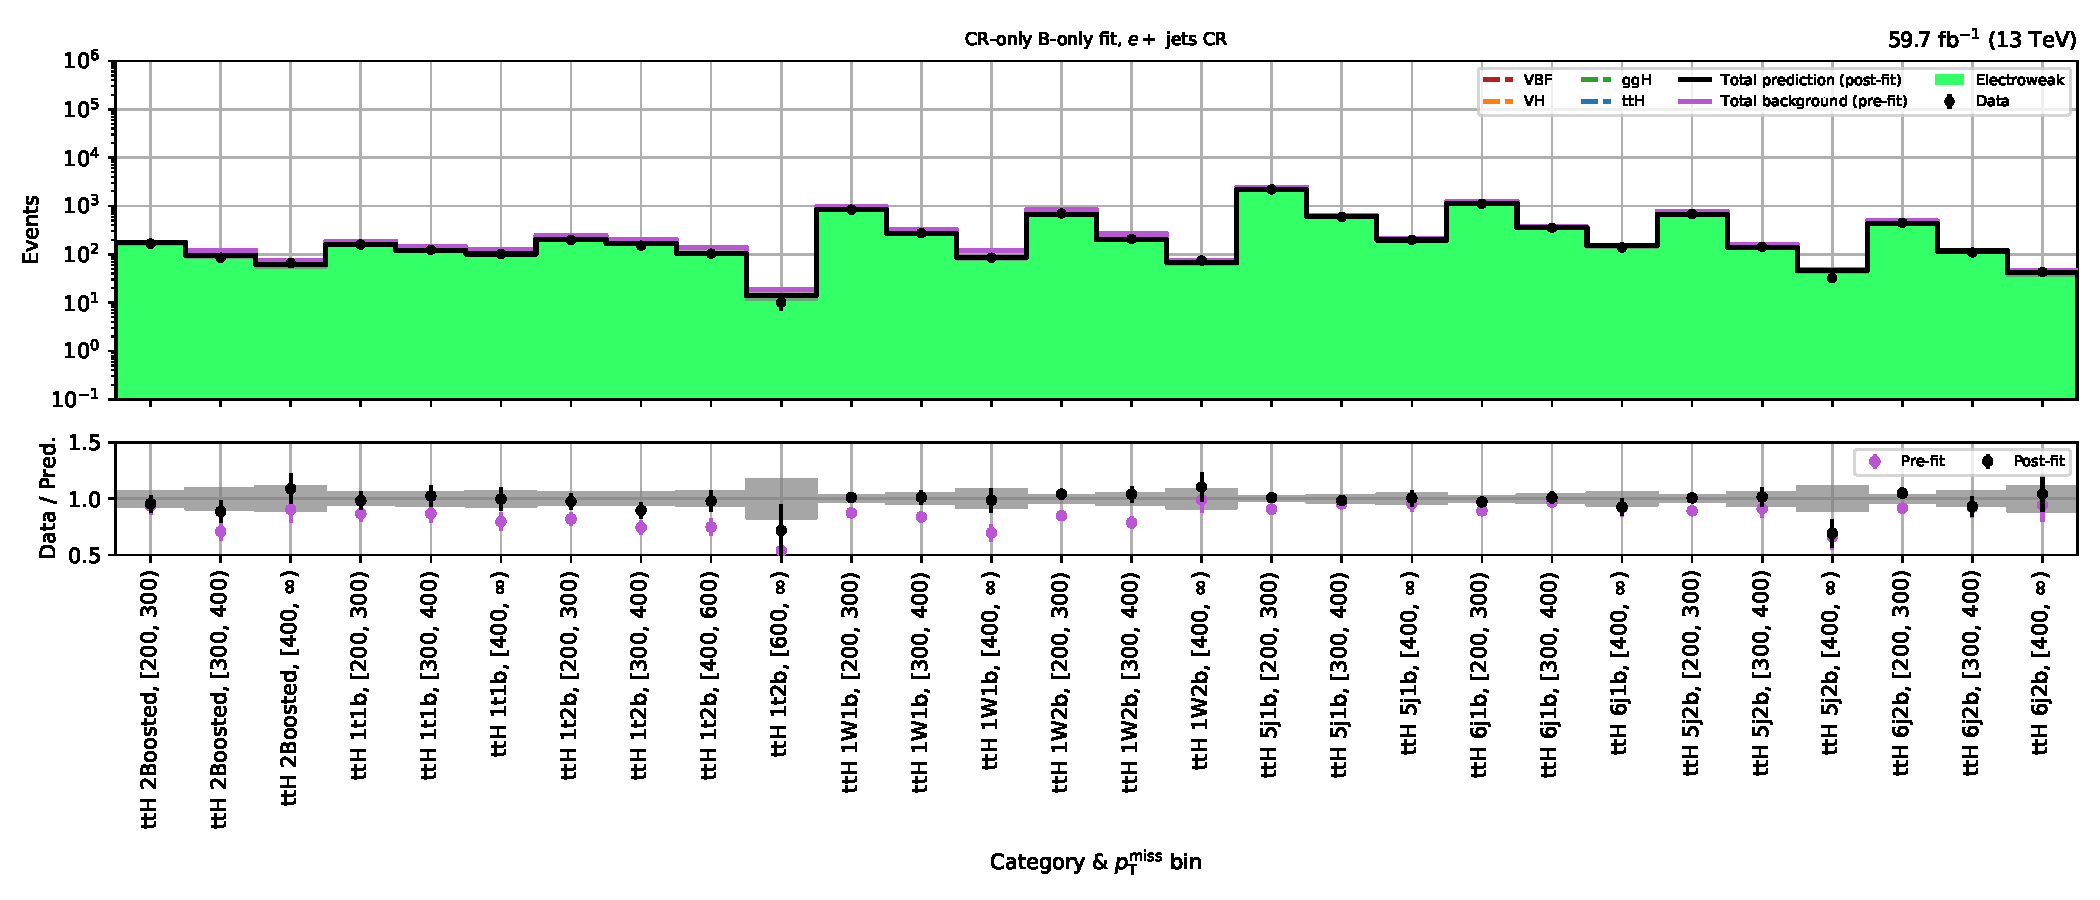
\includegraphics[width=\textwidth]{chapters/higgstoinv/figures/mountain_ranges/2018/ttH/Wenu_tree_fit_b-abs_values_ttH_cats.pdf}
        \caption{\ttH --- \singleEleCr \gls{CR} (2018)}
    \end{subfigure}

    \begin{subfigure}[b]{0.65\textwidth}
        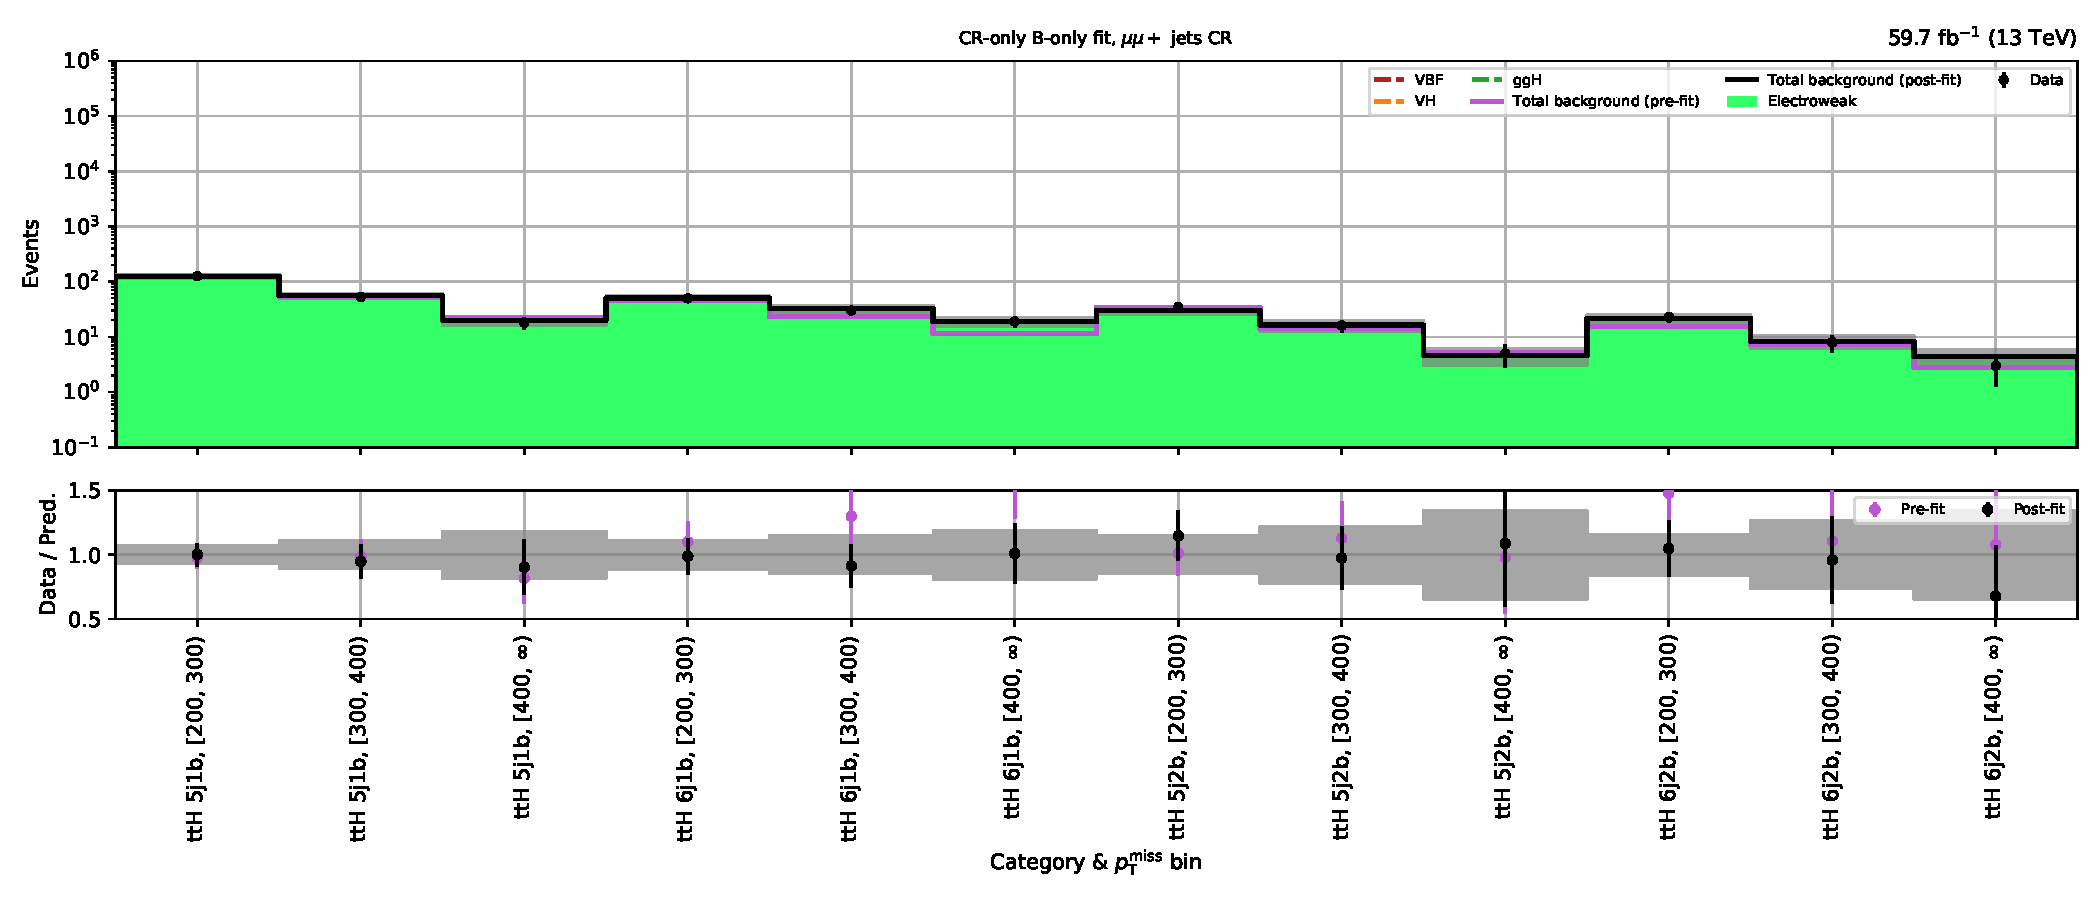
\includegraphics[width=\textwidth]{chapters/higgstoinv/figures/mountain_ranges/2018/ttH/Zmumu_tree_fit_b-abs_values_ttH_cats.pdf}
        \caption{\ttH --- \doubleMuCr \gls{CR} (2018)}
    \end{subfigure}

    \begin{subfigure}[b]{0.65\textwidth}
        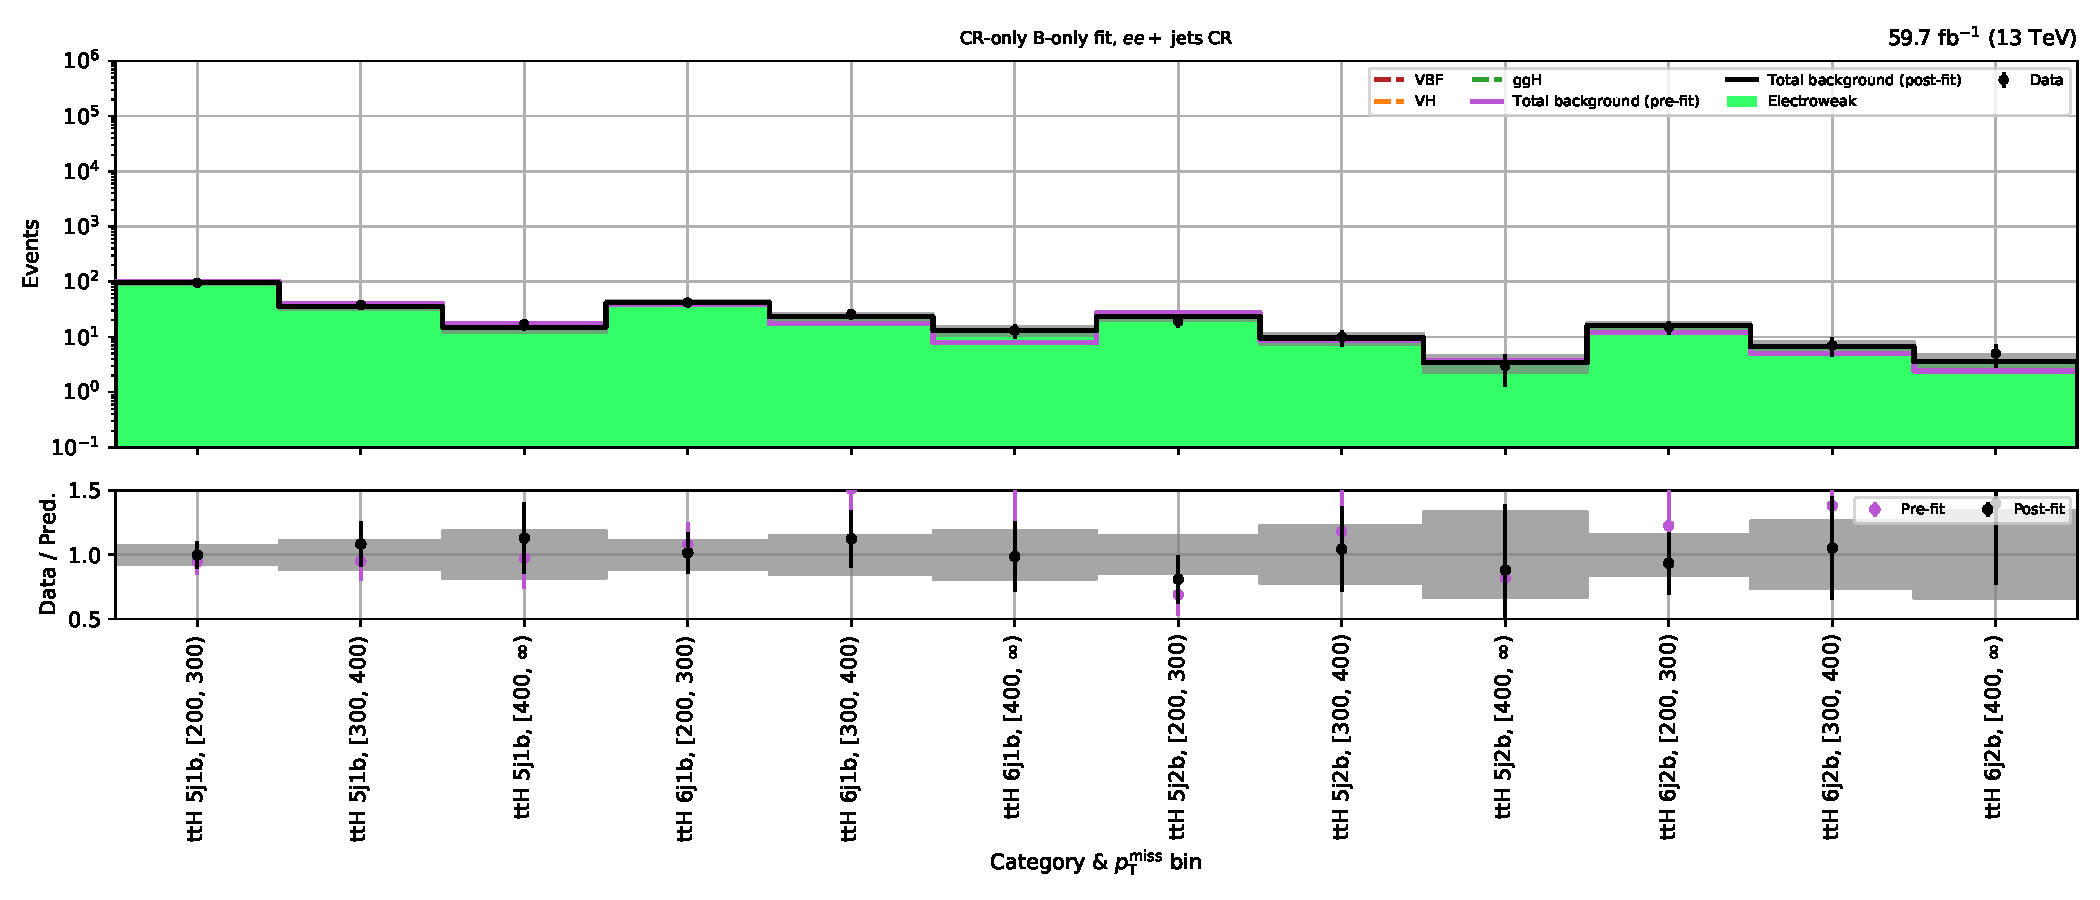
\includegraphics[width=\textwidth]{chapters/higgstoinv/figures/mountain_ranges/2018/ttH/Zee_tree_fit_b-abs_values_ttH_cats.pdf}
        \caption{\ttH --- \doubleEleCr \gls{CR} (2018)}
    \end{subfigure}
    \caption[Post-fit yields for each \ttH category and \ptmiss bin in the lepton control regions for the 2018 dataset]{Post-fit yields for each \ttH category and \ptmiss bin in the lepton \glspl{CR} for the 2018 dataset. The total background pre-fit and post-fit is compared to data in the lower panel of each subfigure.}
    \label{fig:htoinv_mountain_range_ttH_2018_CRs}
\end{figure}

\clearpage


%=========================================================


\section{Control region-only fits to the \texorpdfstring{\VH}{VH} categories}
\label{sec:pre_post_fit_plots_VH_CRs}

\begin{figure}[htbp]
    \centering
    \begin{subfigure}[b]{0.49\textwidth}
        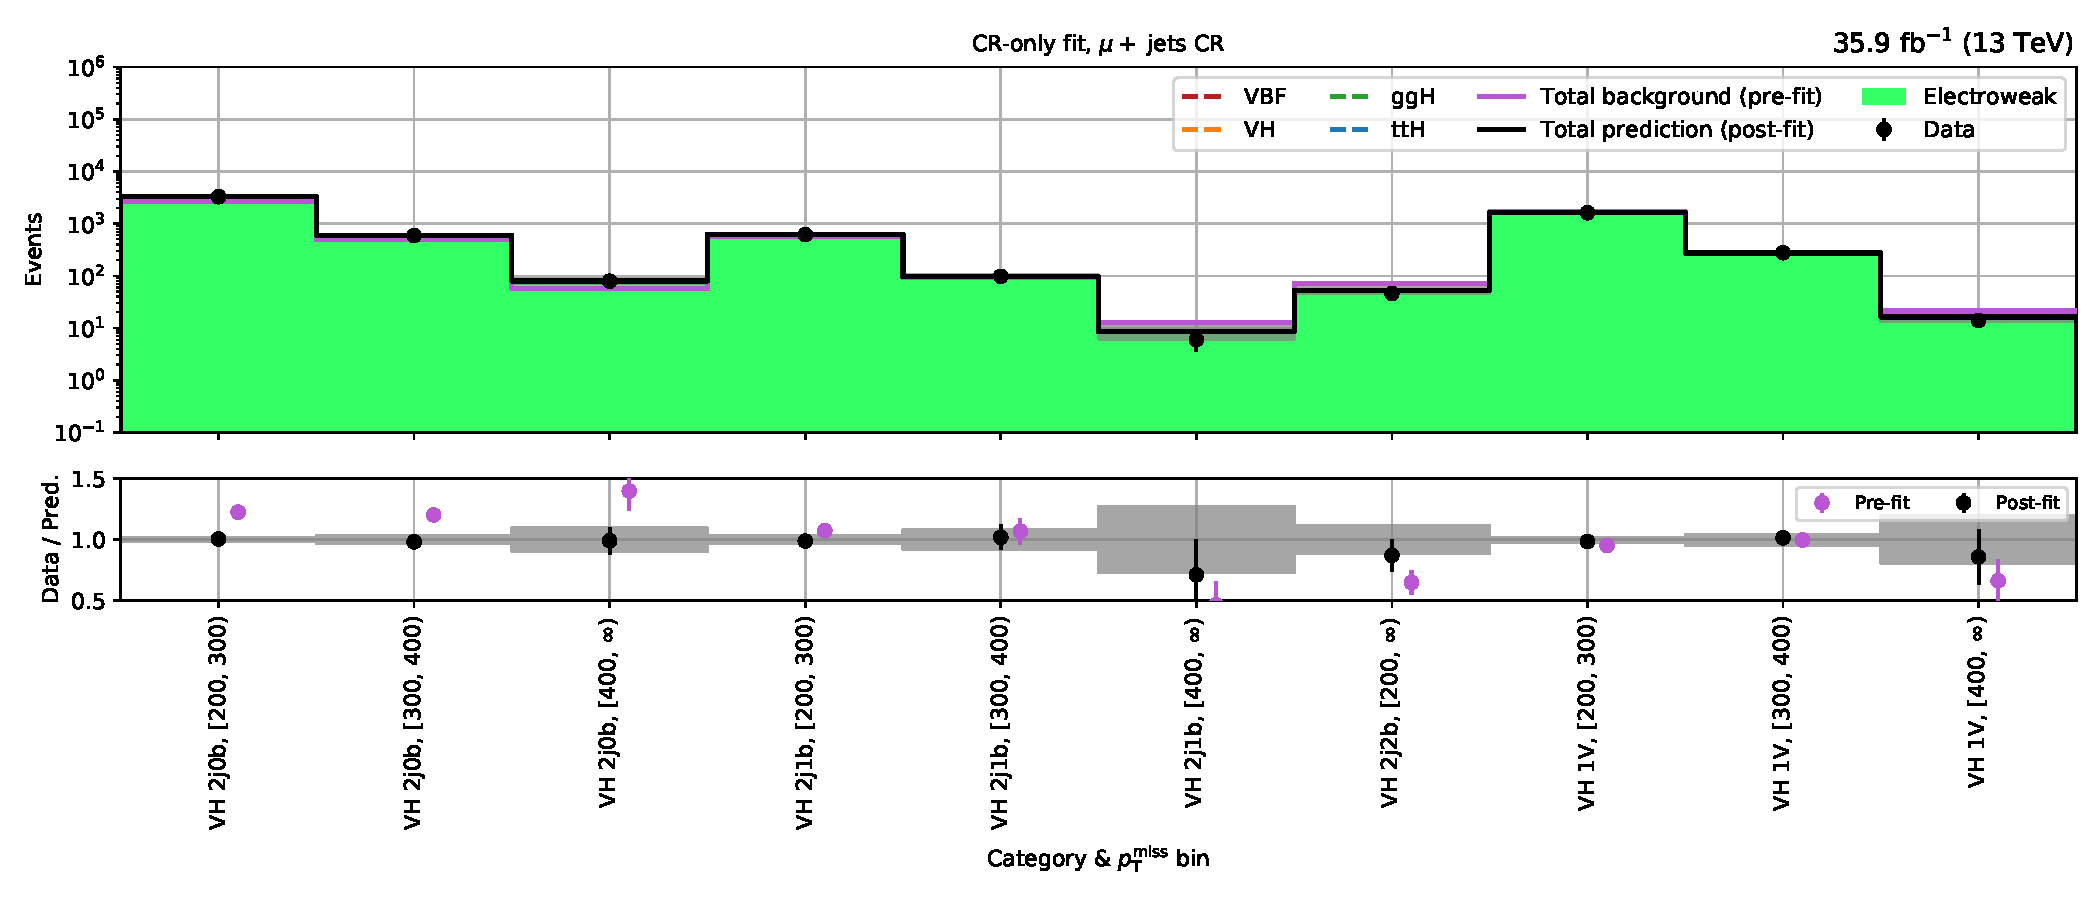
\includegraphics[width=\textwidth]{chapters/higgstoinv/figures/mountain_ranges/2016/VH/Wmunu_tree_fit_b-abs_values_VH_cats.pdf}
        \caption{\VH --- \singleMuCr \gls{CR} (2016)}
    \end{subfigure}
    \hfill
    \begin{subfigure}[b]{0.49\textwidth}
        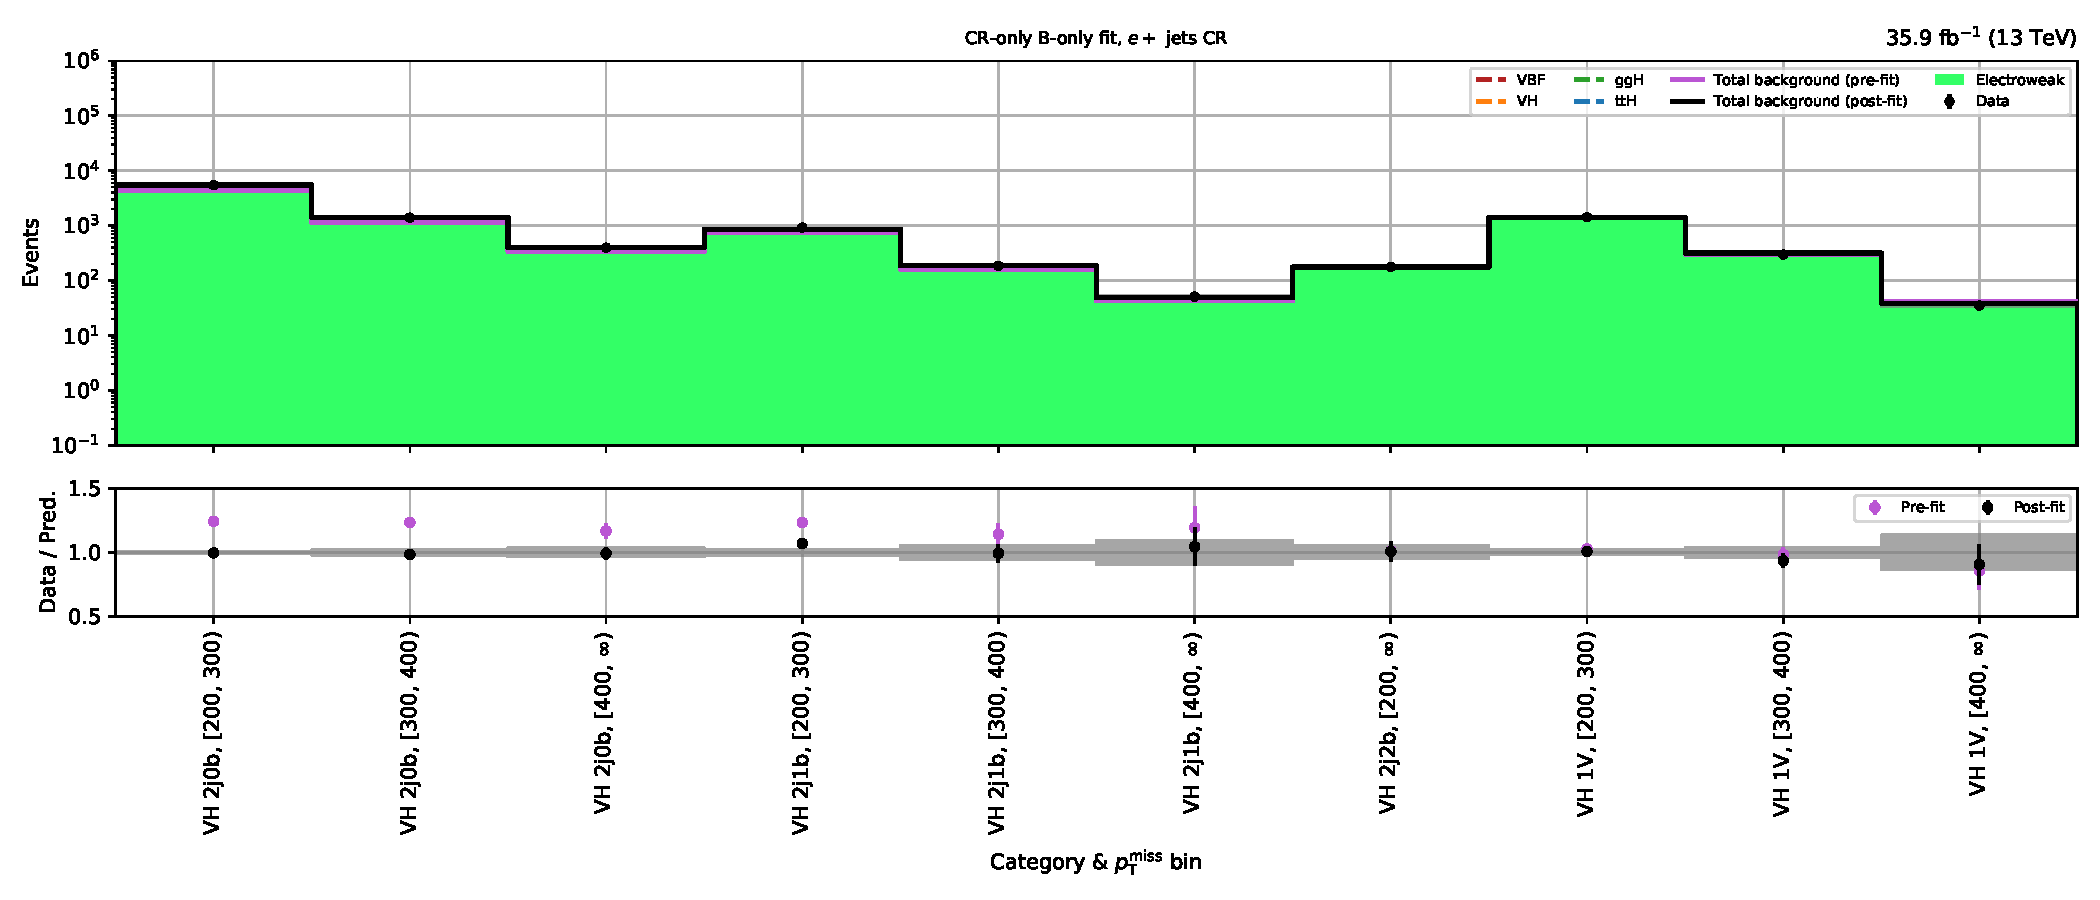
\includegraphics[width=\textwidth]{chapters/higgstoinv/figures/mountain_ranges/2016/VH/Wenu_tree_fit_b-abs_values_VH_cats.pdf}
        \caption{\VH --- \singleEleCr \gls{CR} (2016)}
    \end{subfigure}

    \begin{subfigure}[b]{0.49\textwidth}
        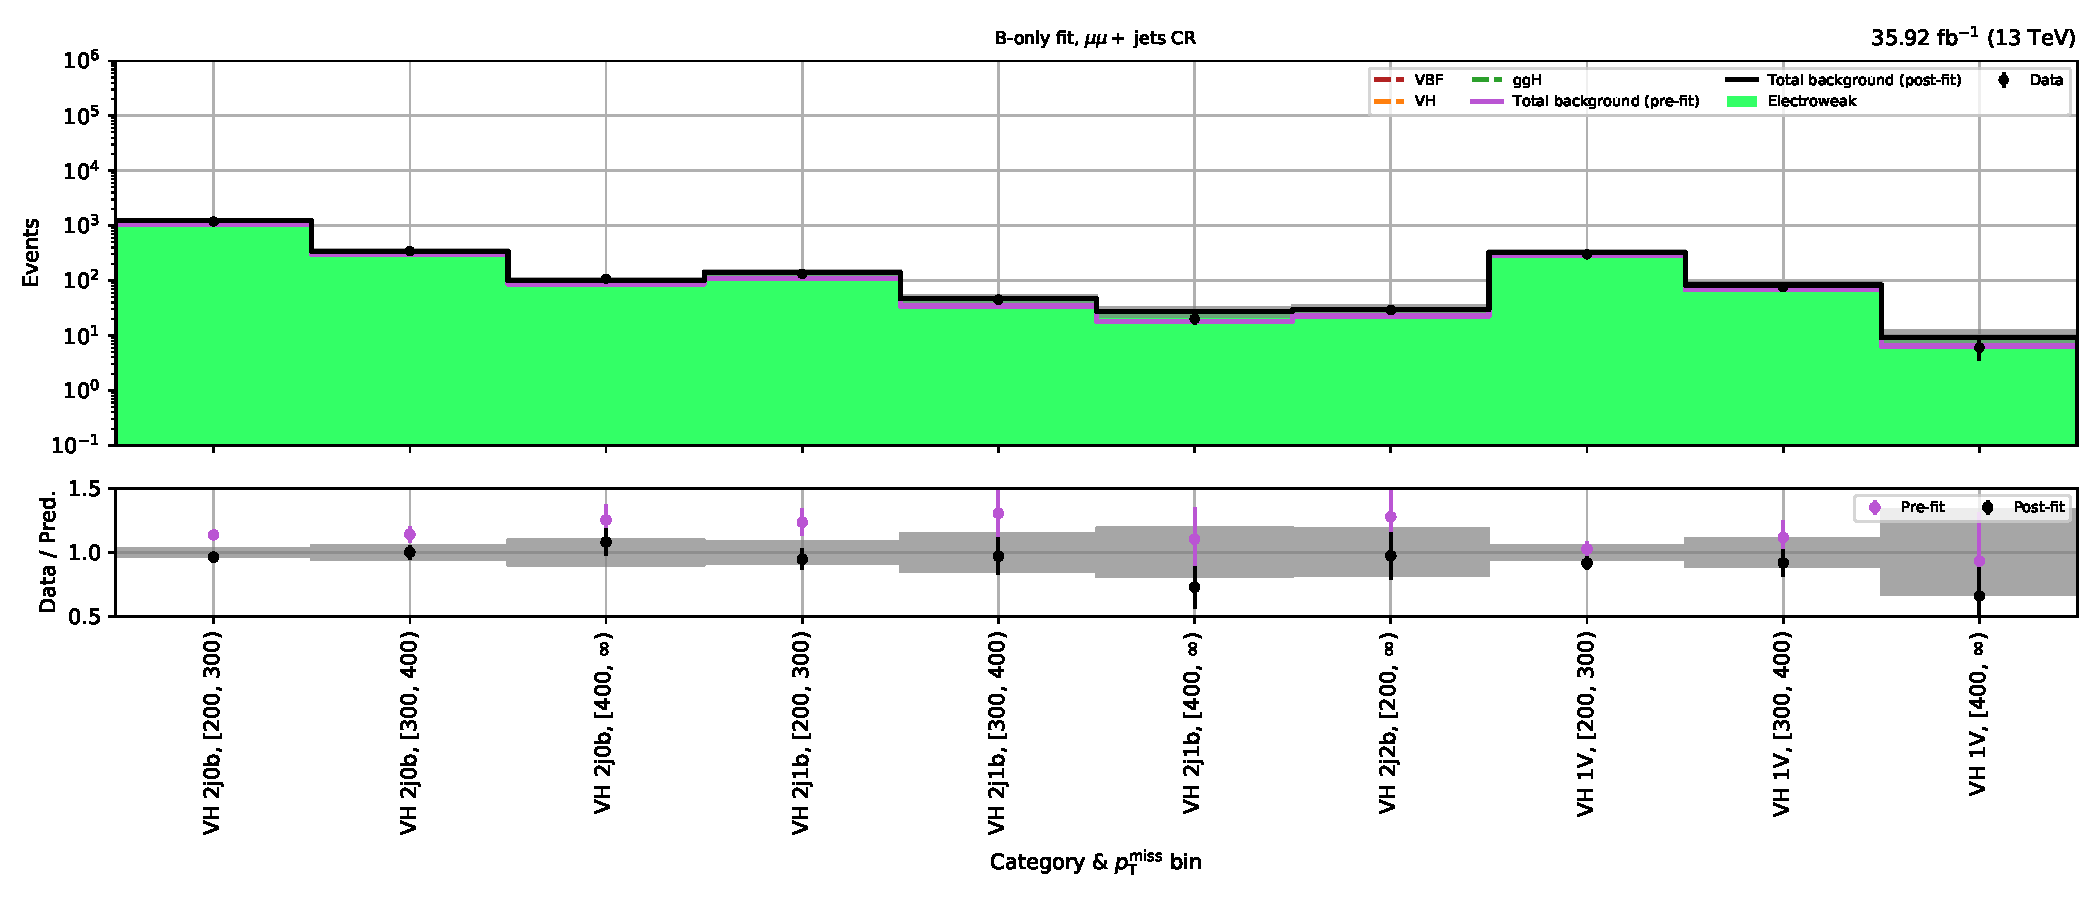
\includegraphics[width=\textwidth]{chapters/higgstoinv/figures/mountain_ranges/2016/VH/Zmumu_tree_fit_b-abs_values_VH_cats.pdf}
        \caption{\VH --- \doubleMuCr \gls{CR} (2016)}
    \end{subfigure}
    \hfill
    \begin{subfigure}[b]{0.49\textwidth}
        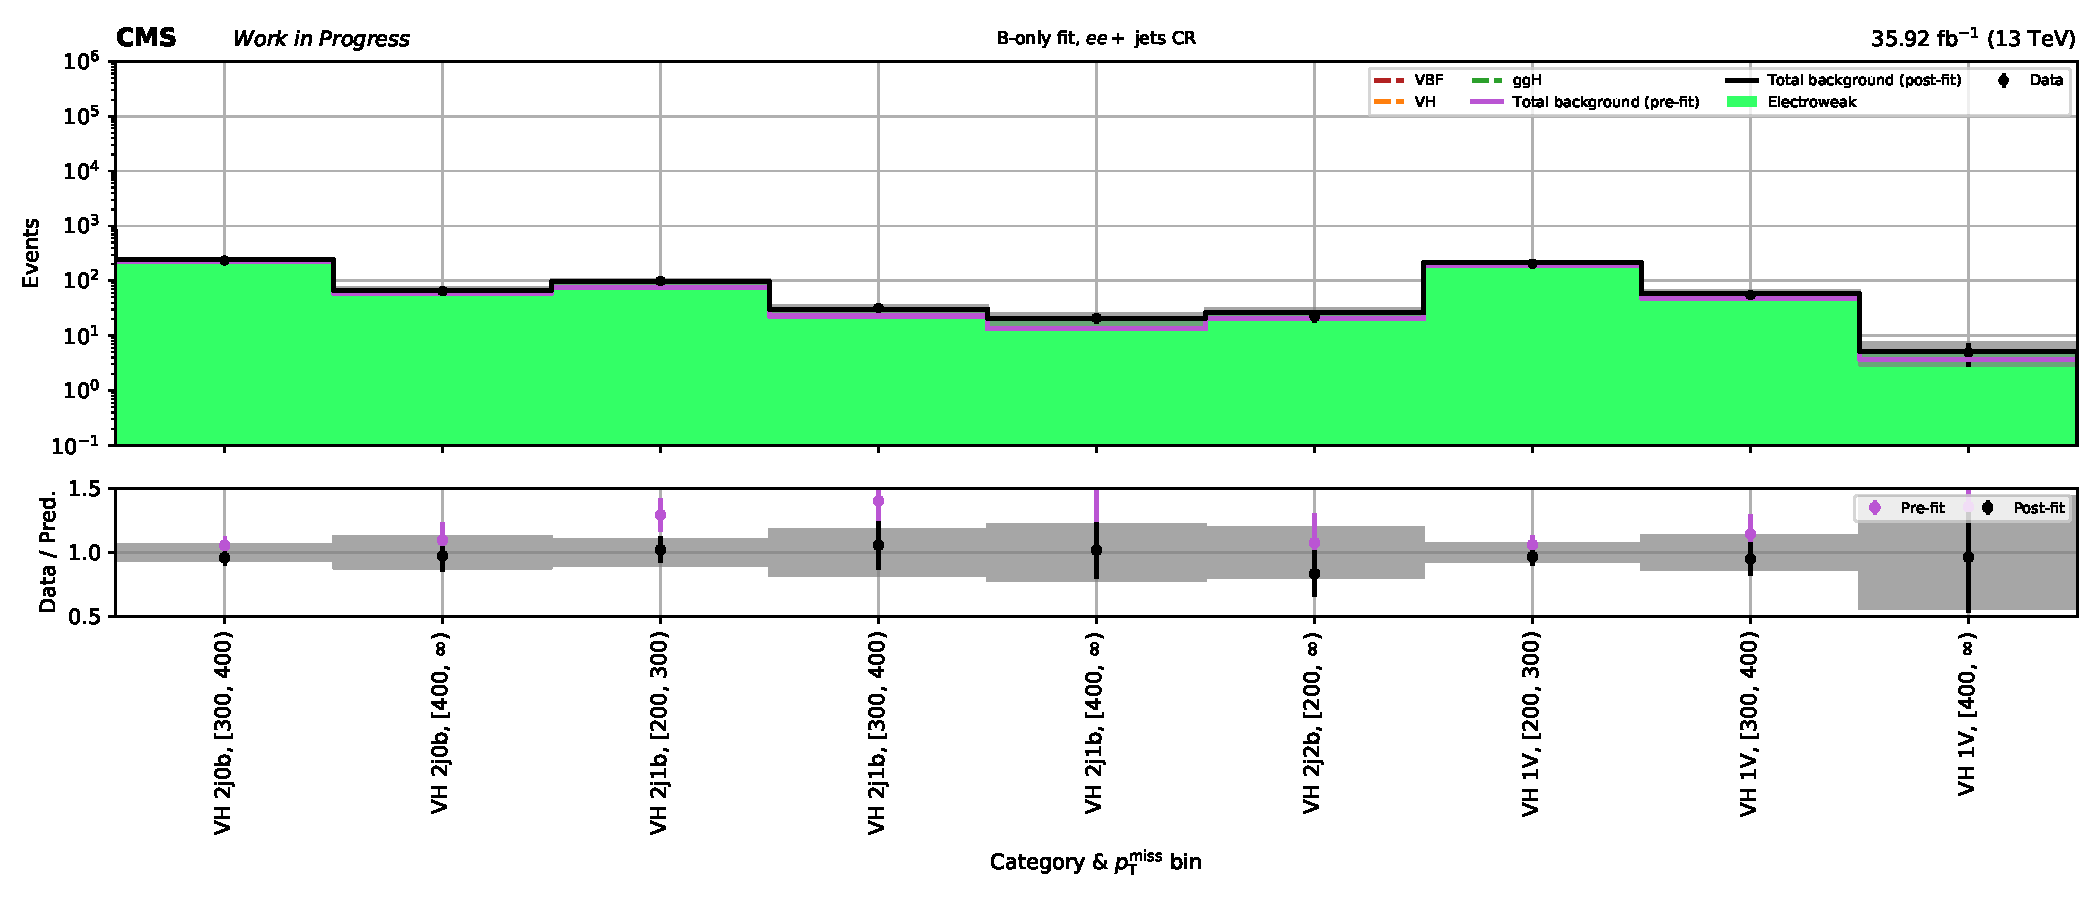
\includegraphics[width=\textwidth]{chapters/higgstoinv/figures/mountain_ranges/2016/VH/Zee_tree_fit_b-abs_values_VH_cats.pdf}
        \caption{\VH --- \doubleEleCr \gls{CR} (2016)}
    \end{subfigure}

    \begin{subfigure}[b]{0.49\textwidth}
        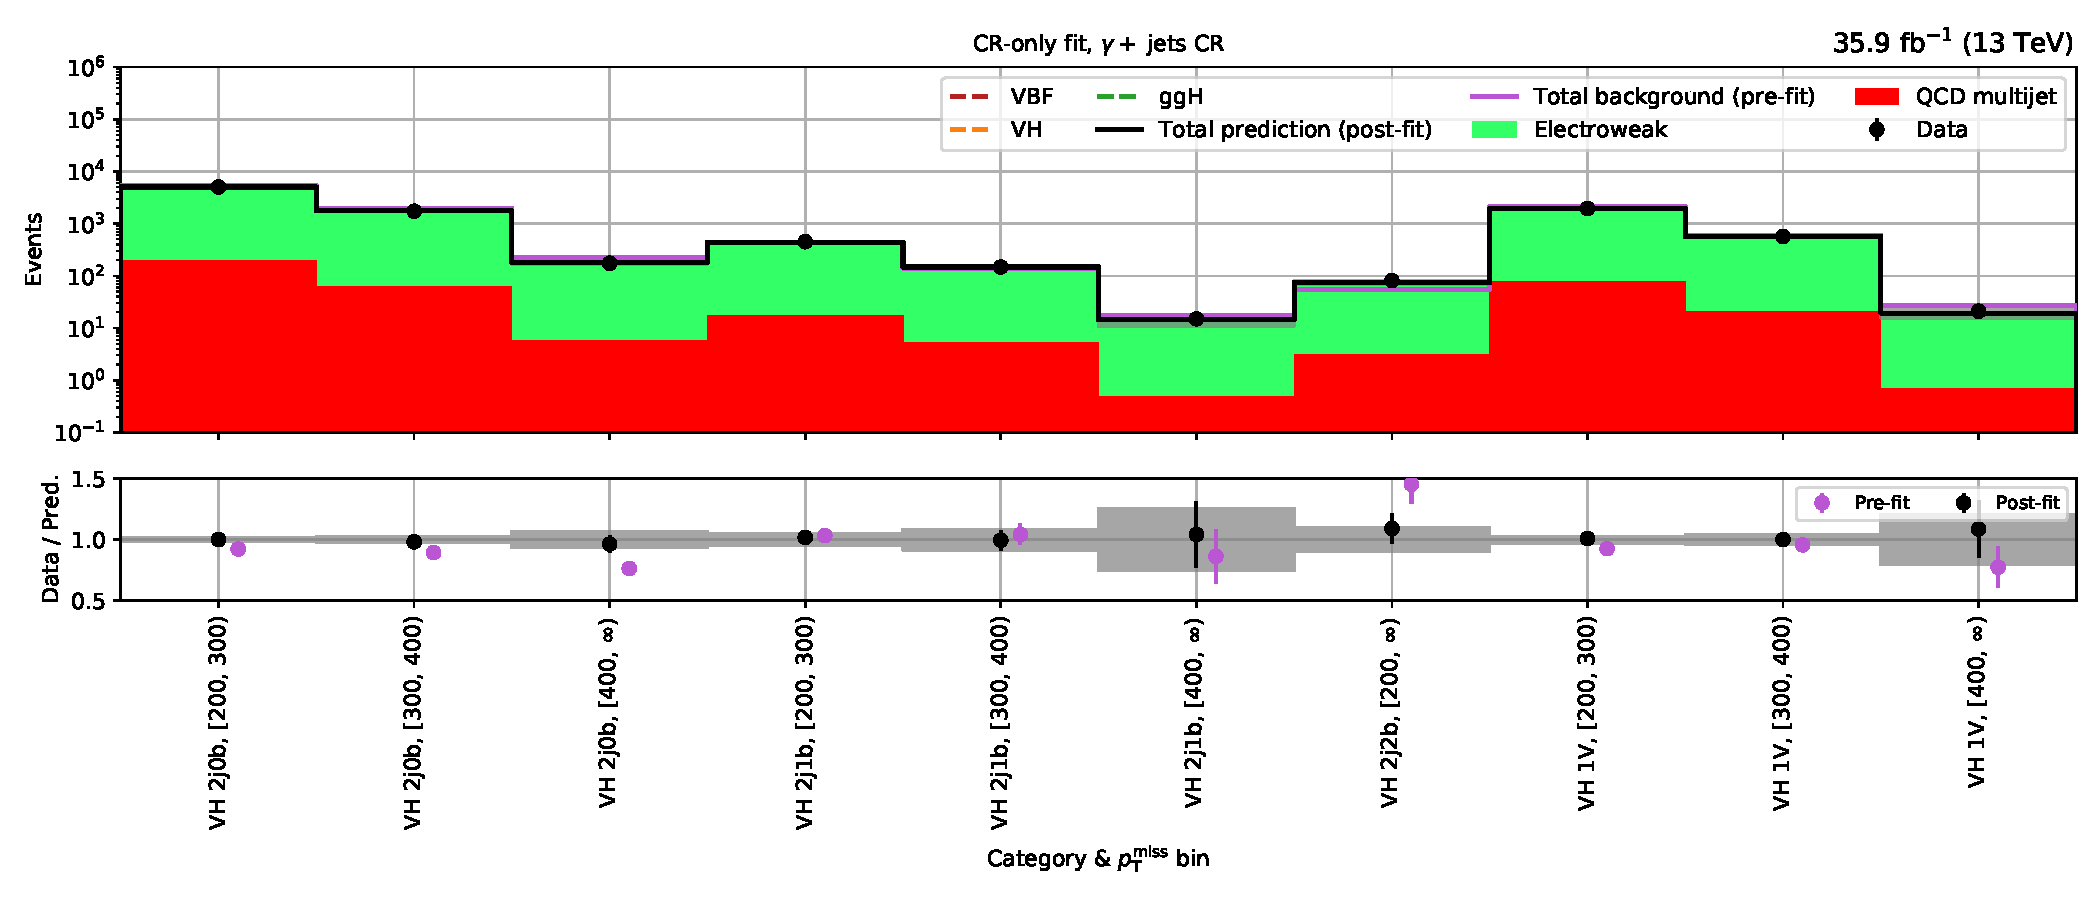
\includegraphics[width=\textwidth]{chapters/higgstoinv/figures/mountain_ranges/2016/VH/Photon_tree_fit_b-abs_values_VH_cats.pdf}
        \caption{\VH --- \singlePhotonCr \gls{CR} (2016)}
    \end{subfigure}
    \caption[Post-fit yields for each \VH category and \ptmiss bin in the lepton and photon control regions for the 2016 dataset]{Post-fit yields for each \VH category and \ptmiss bin in the lepton and photon \glspl{CR} for the 2016 dataset. The total background pre-fit and post-fit is compared to data in the lower panel of each subfigure.}
    \label{fig:htoinv_mountain_range_VH_2016_CRs}
\end{figure}

\begin{figure}[htbp]
    \centering
    \begin{subfigure}[b]{0.49\textwidth}
        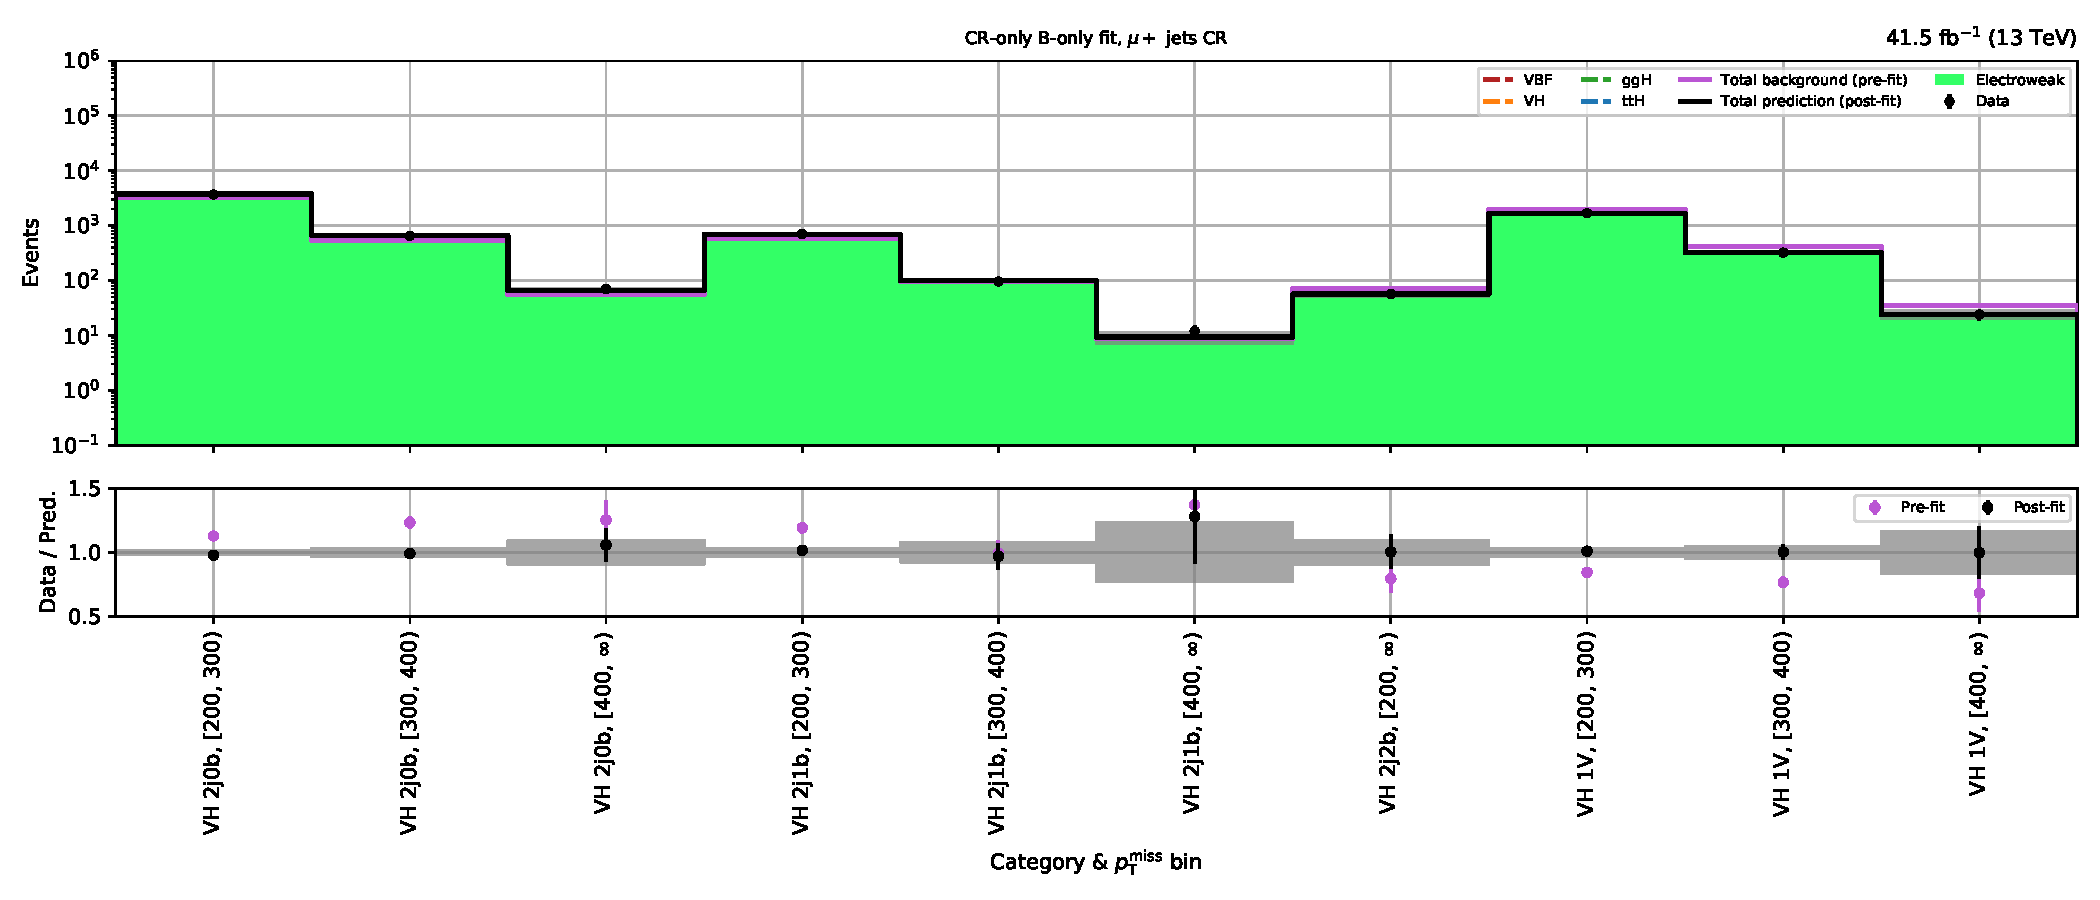
\includegraphics[width=\textwidth]{chapters/higgstoinv/figures/mountain_ranges/2017/VH/Wmunu_tree_fit_b-abs_values_VH_cats.pdf}
        \caption{\VH --- \singleMuCr \gls{CR} (2017)}
    \end{subfigure}
    \hfill
    \begin{subfigure}[b]{0.49\textwidth}
        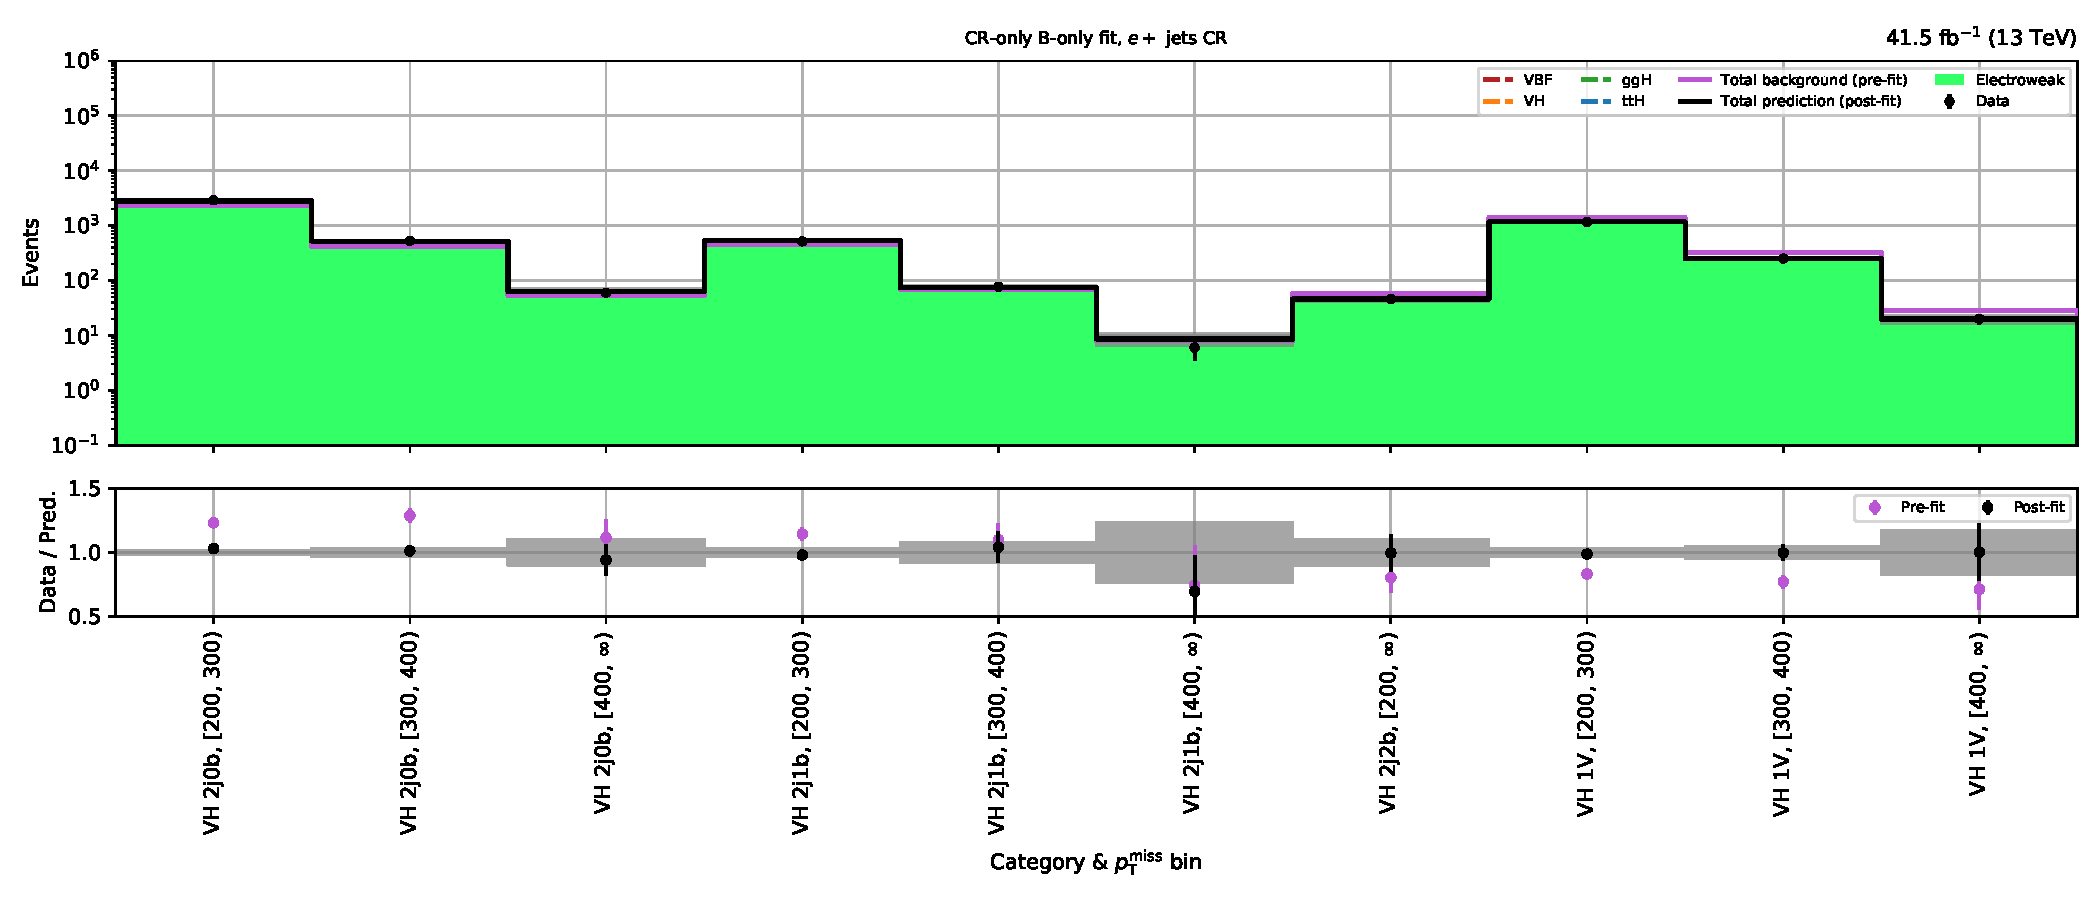
\includegraphics[width=\textwidth]{chapters/higgstoinv/figures/mountain_ranges/2017/VH/Wenu_tree_fit_b-abs_values_VH_cats.pdf}
        \caption{\VH --- \singleEleCr \gls{CR} (2017)}
    \end{subfigure}

    \begin{subfigure}[b]{0.49\textwidth}
        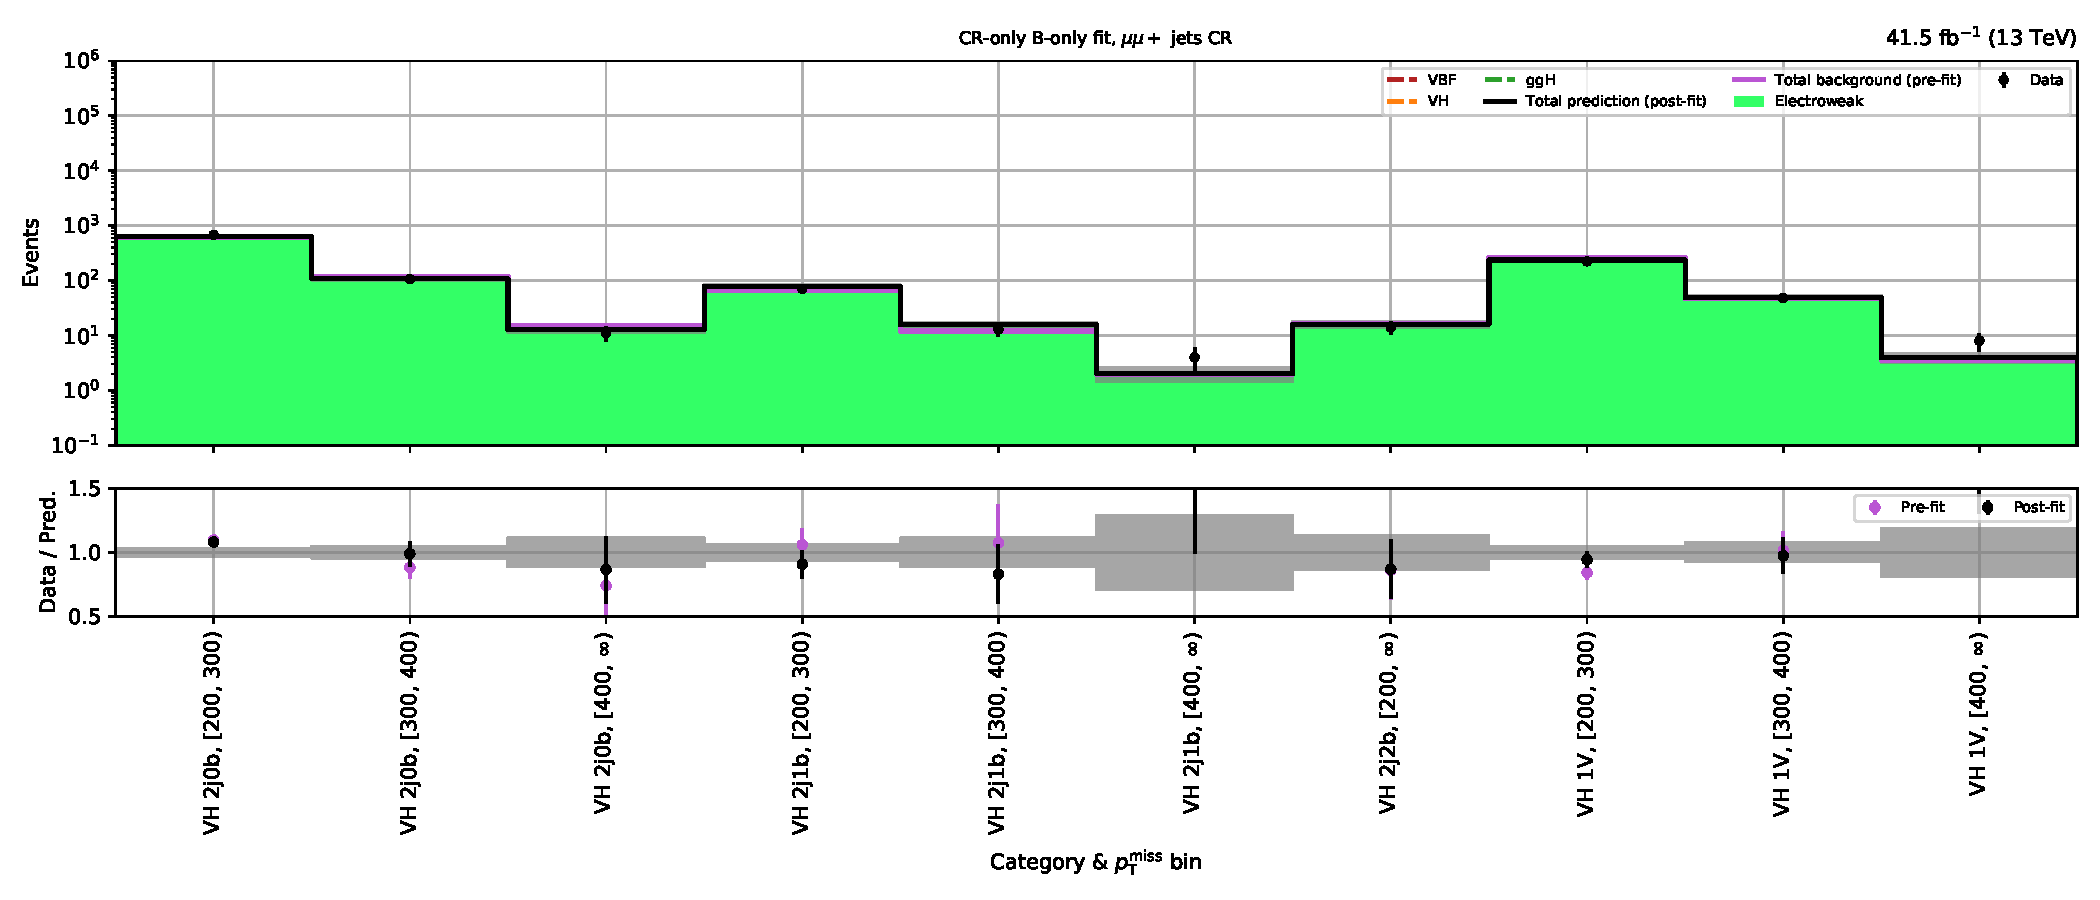
\includegraphics[width=\textwidth]{chapters/higgstoinv/figures/mountain_ranges/2017/VH/Zmumu_tree_fit_b-abs_values_VH_cats.pdf}
        \caption{\VH --- \doubleMuCr \gls{CR} (2017)}
    \end{subfigure}
    \hfill
    \begin{subfigure}[b]{0.49\textwidth}
        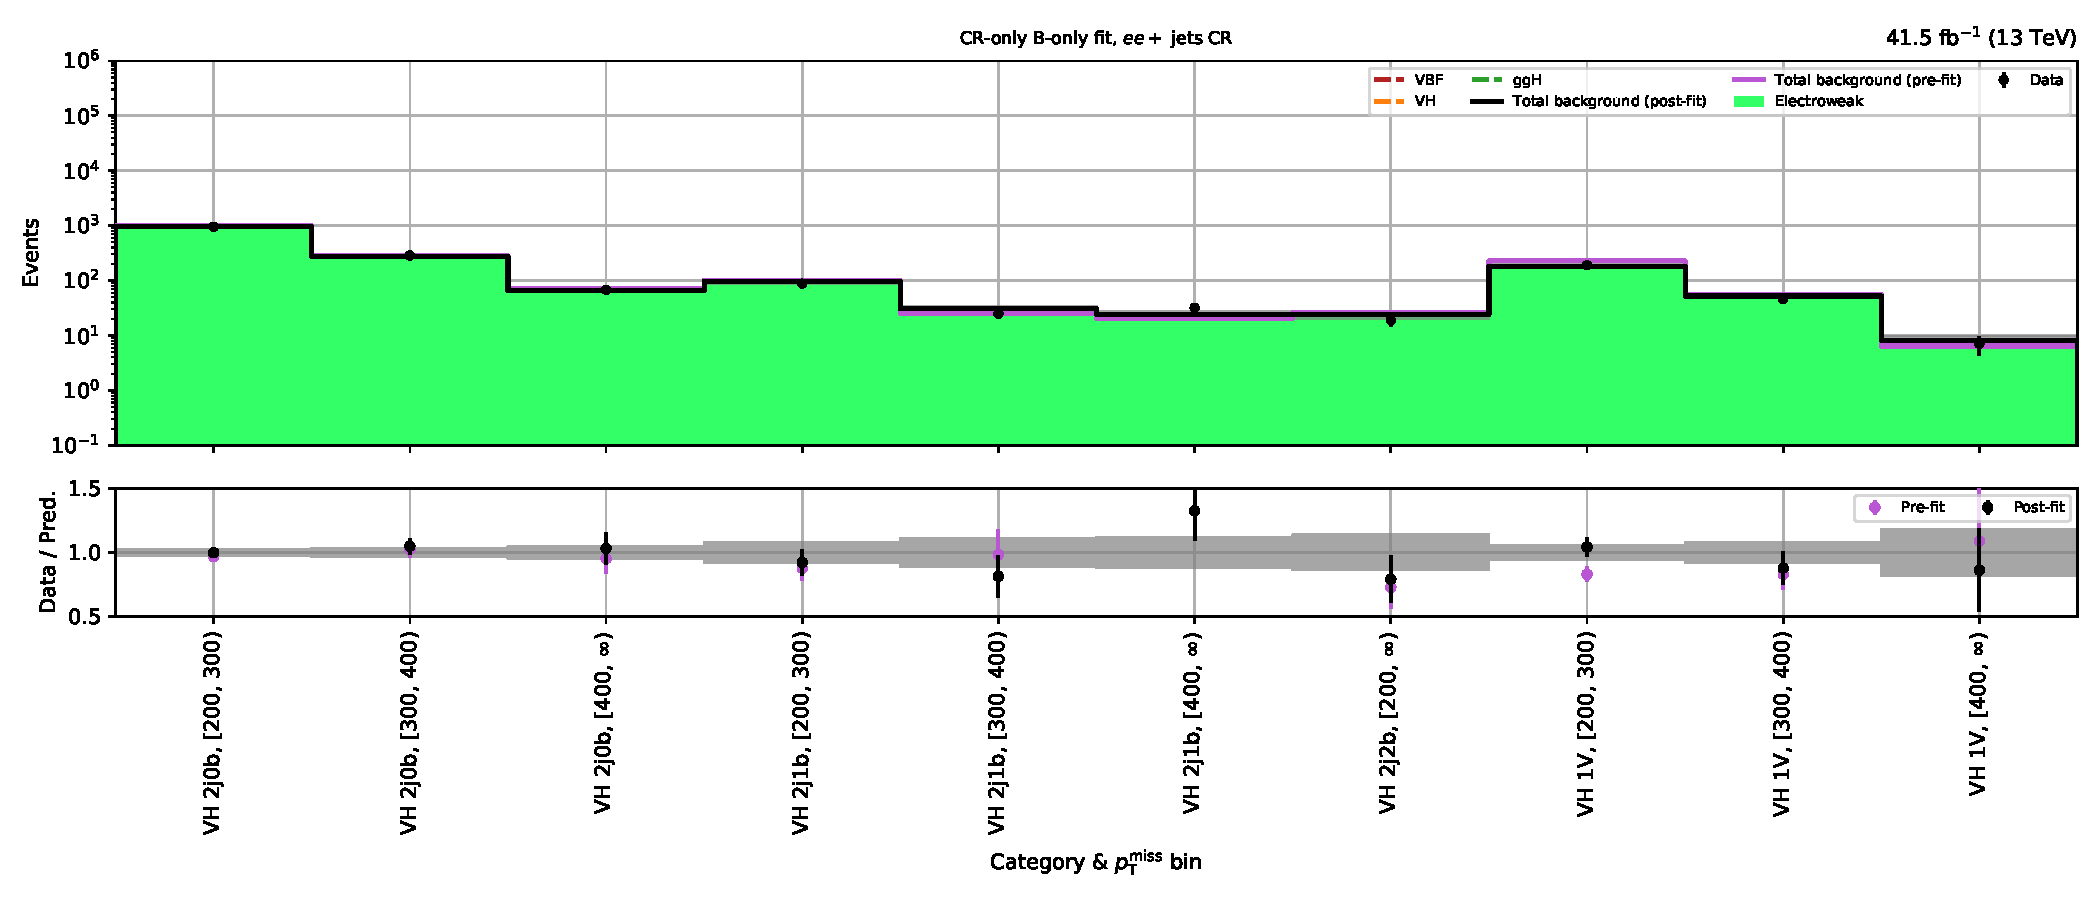
\includegraphics[width=\textwidth]{chapters/higgstoinv/figures/mountain_ranges/2017/VH/Zee_tree_fit_b-abs_values_VH_cats.pdf}
        \caption{\VH --- \doubleEleCr \gls{CR} (2017)}
    \end{subfigure}

    \begin{subfigure}[b]{0.49\textwidth}
        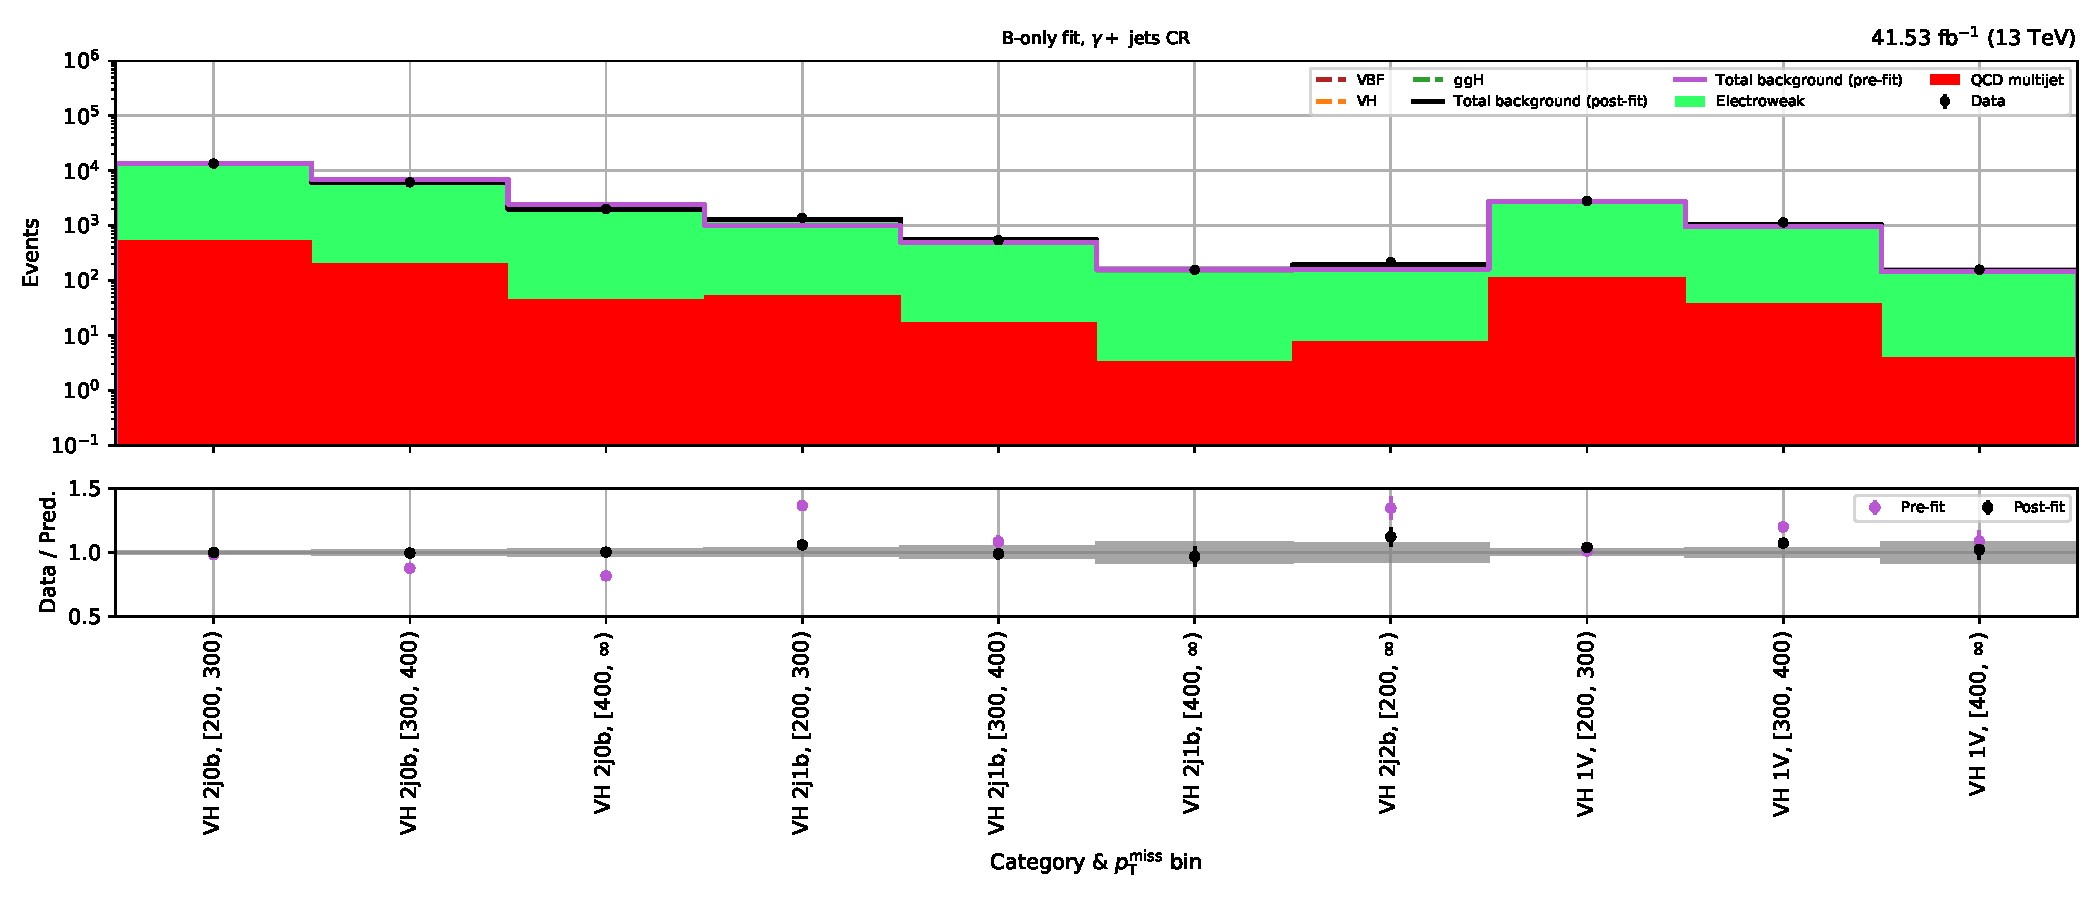
\includegraphics[width=\textwidth]{chapters/higgstoinv/figures/mountain_ranges/2017/VH/Photon_tree_fit_b-abs_values_VH_cats.pdf}
        \caption{\VH --- \singlePhotonCr \gls{CR} (2017)}
    \end{subfigure}
    \caption[Post-fit yields for each \VH category and \ptmiss bin in the lepton and photon control regions for the 2017 dataset]{Post-fit yields for each \VH category and \ptmiss bin in the lepton and photon \glspl{CR} for the 2017 dataset. The total background pre-fit and post-fit is compared to data in the lower panel of each subfigure.}
    \label{fig:htoinv_mountain_range_VH_2017_CRs}
\end{figure}

\begin{figure}[htbp]
    \centering
    \begin{subfigure}[b]{0.49\textwidth}
        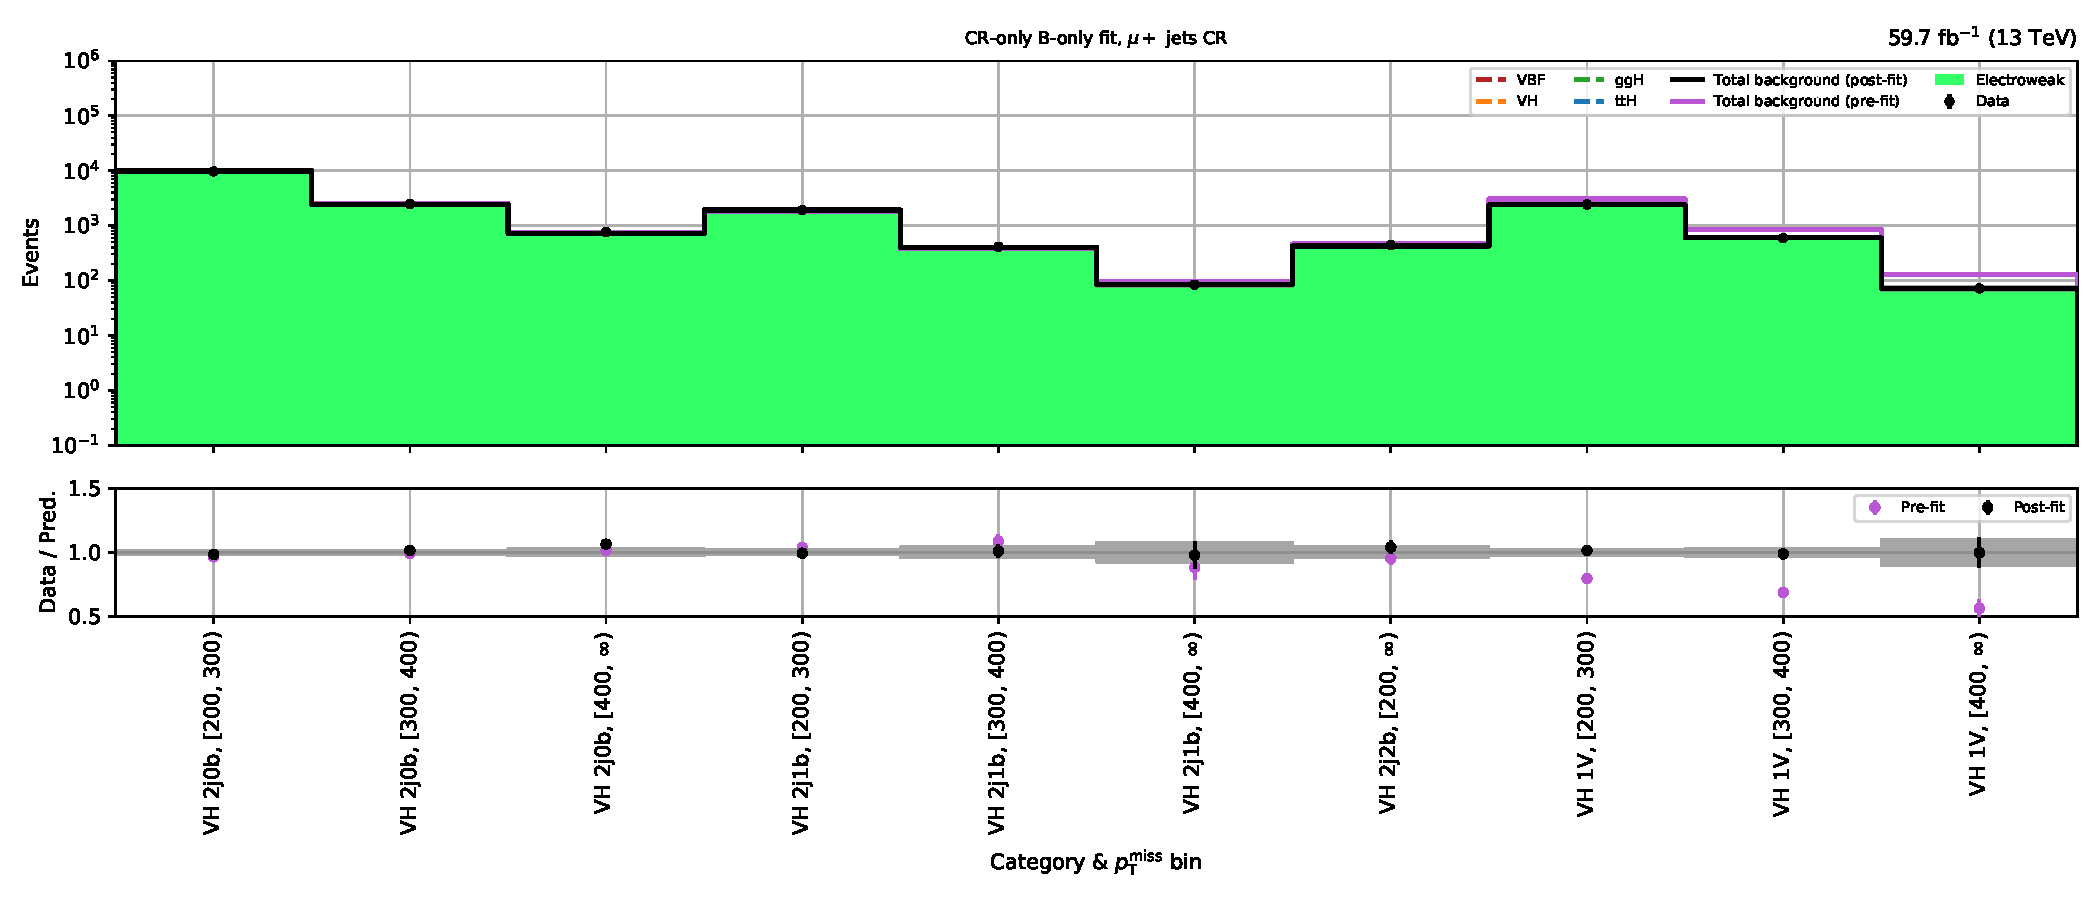
\includegraphics[width=\textwidth]{chapters/higgstoinv/figures/mountain_ranges/2018/VH/Wmunu_tree_fit_b-abs_values_VH_cats.pdf}
        \caption{\VH --- \singleMuCr \gls{CR} (2018)}
    \end{subfigure}
    \hfill
    \begin{subfigure}[b]{0.49\textwidth}
        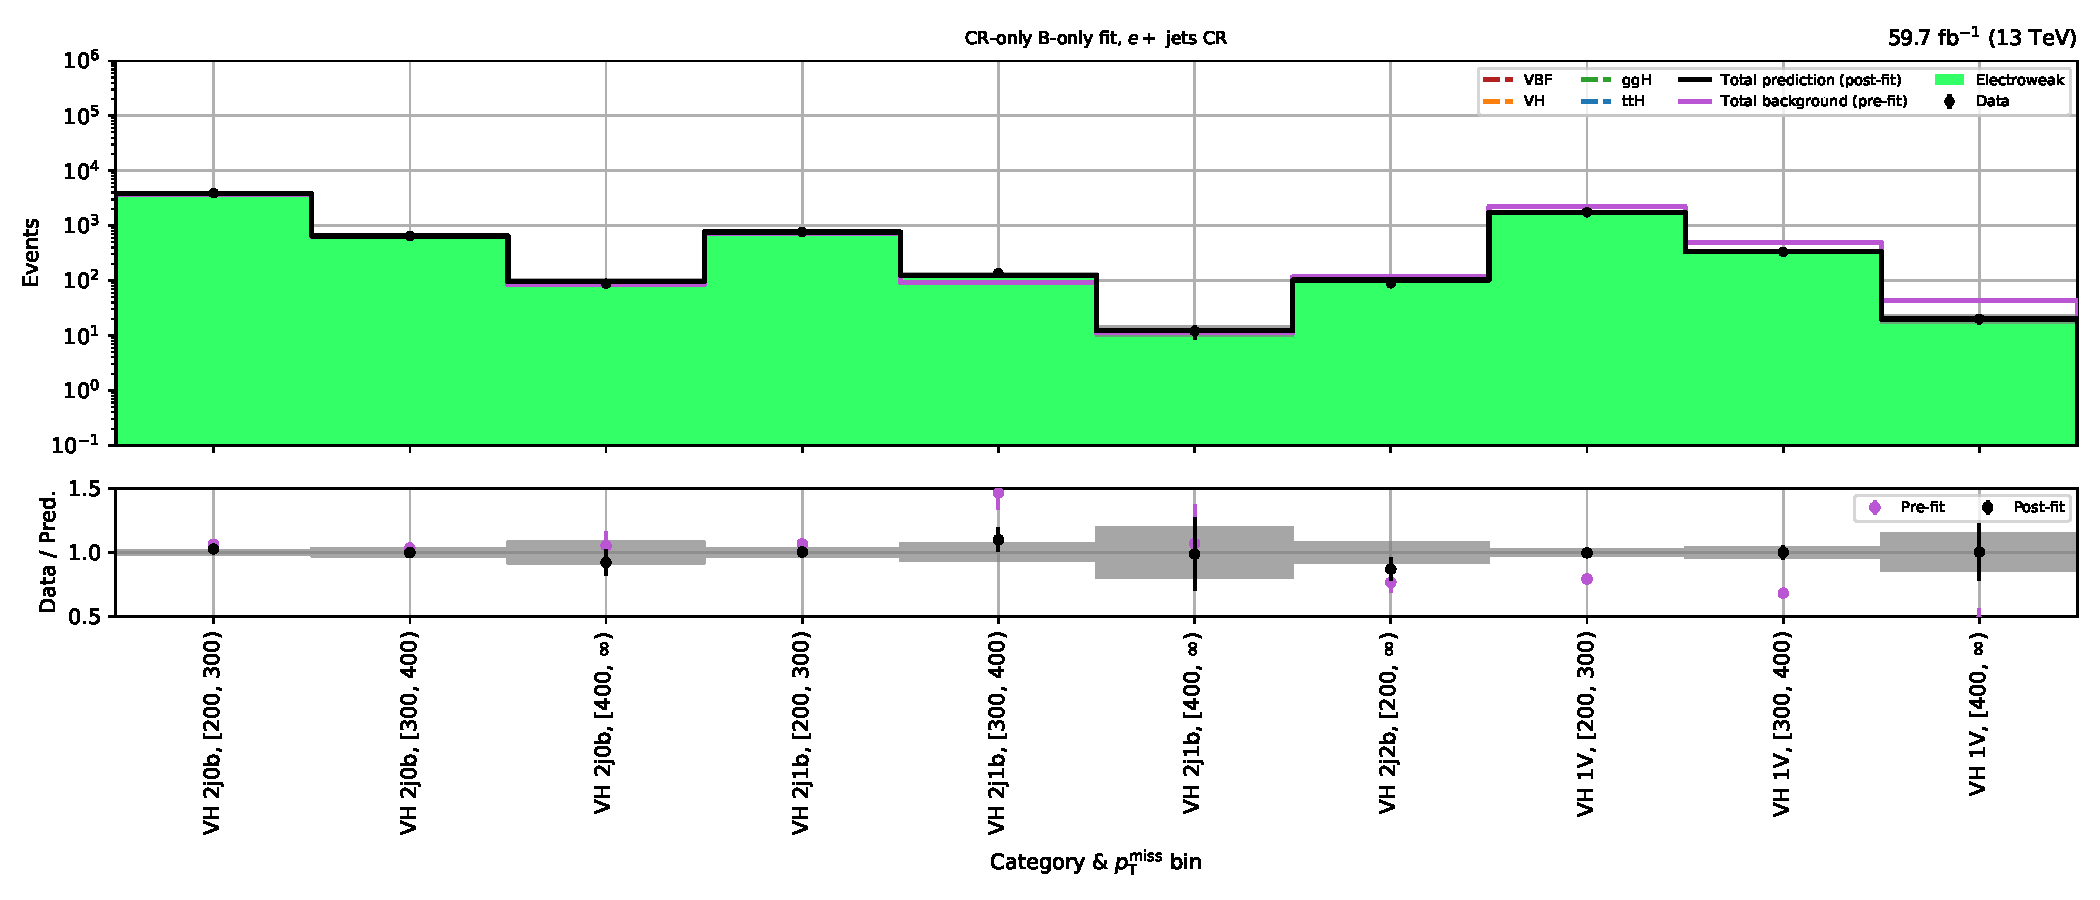
\includegraphics[width=\textwidth]{chapters/higgstoinv/figures/mountain_ranges/2018/VH/Wenu_tree_fit_b-abs_values_VH_cats.pdf}
        \caption{\VH --- \singleEleCr \gls{CR} (2018)}
    \end{subfigure}

    \begin{subfigure}[b]{0.49\textwidth}
        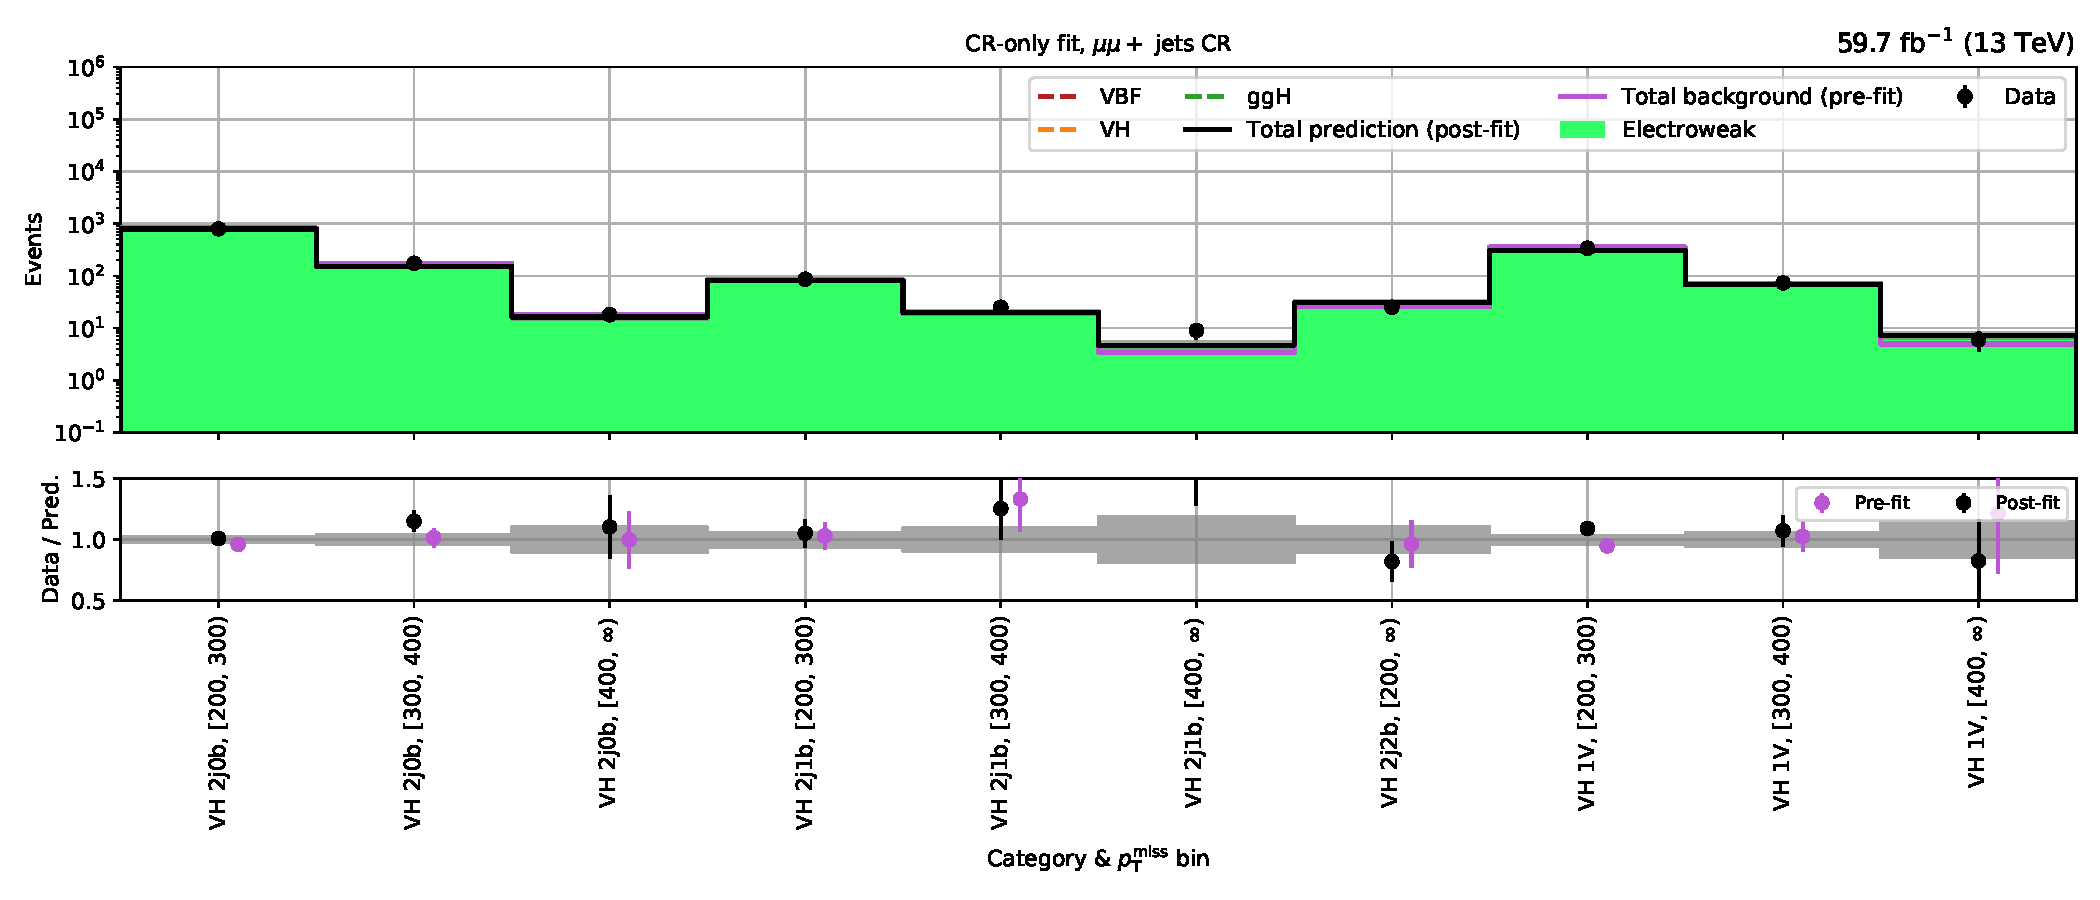
\includegraphics[width=\textwidth]{chapters/higgstoinv/figures/mountain_ranges/2018/VH/Zmumu_tree_fit_b-abs_values_VH_cats.pdf}
        \caption{\VH --- \doubleMuCr \gls{CR} (2018)}
    \end{subfigure}
    \hfill
    \begin{subfigure}[b]{0.49\textwidth}
        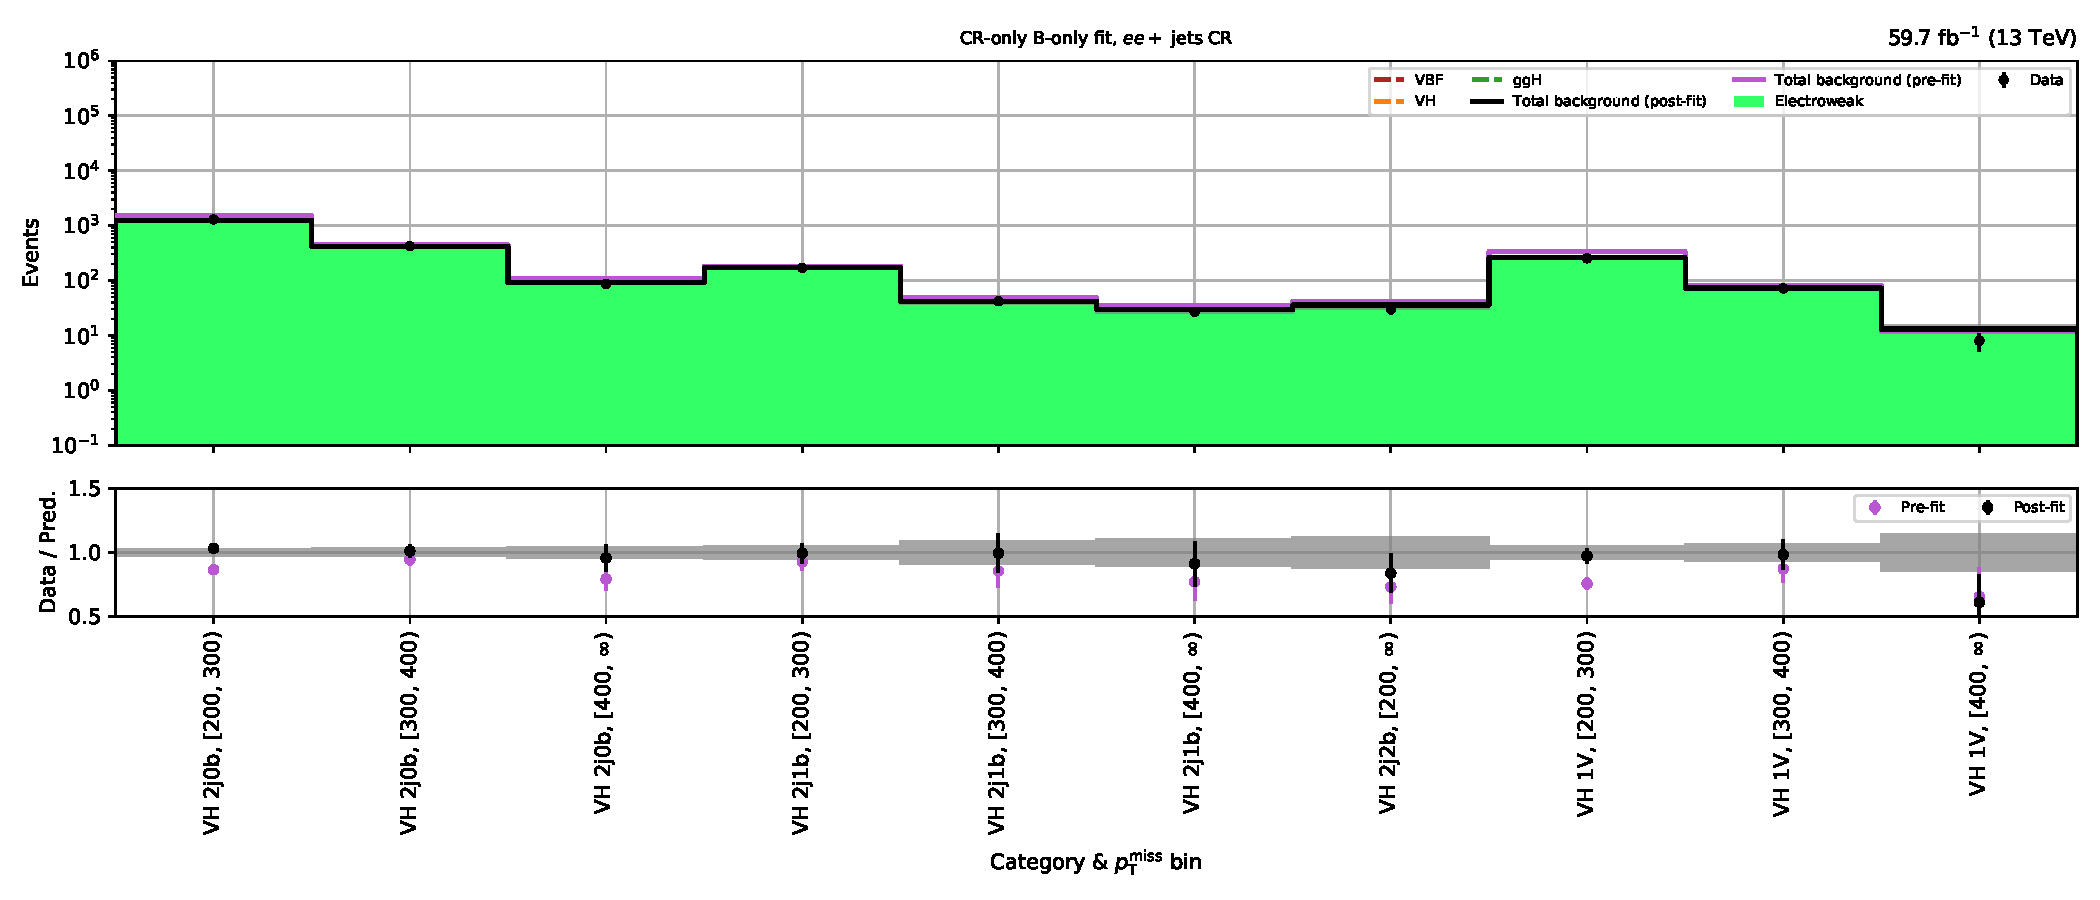
\includegraphics[width=\textwidth]{chapters/higgstoinv/figures/mountain_ranges/2018/VH/Zee_tree_fit_b-abs_values_VH_cats.pdf}
        \caption{\VH --- \doubleEleCr \gls{CR} (2018)}
    \end{subfigure}

    \begin{subfigure}[b]{0.49\textwidth}
        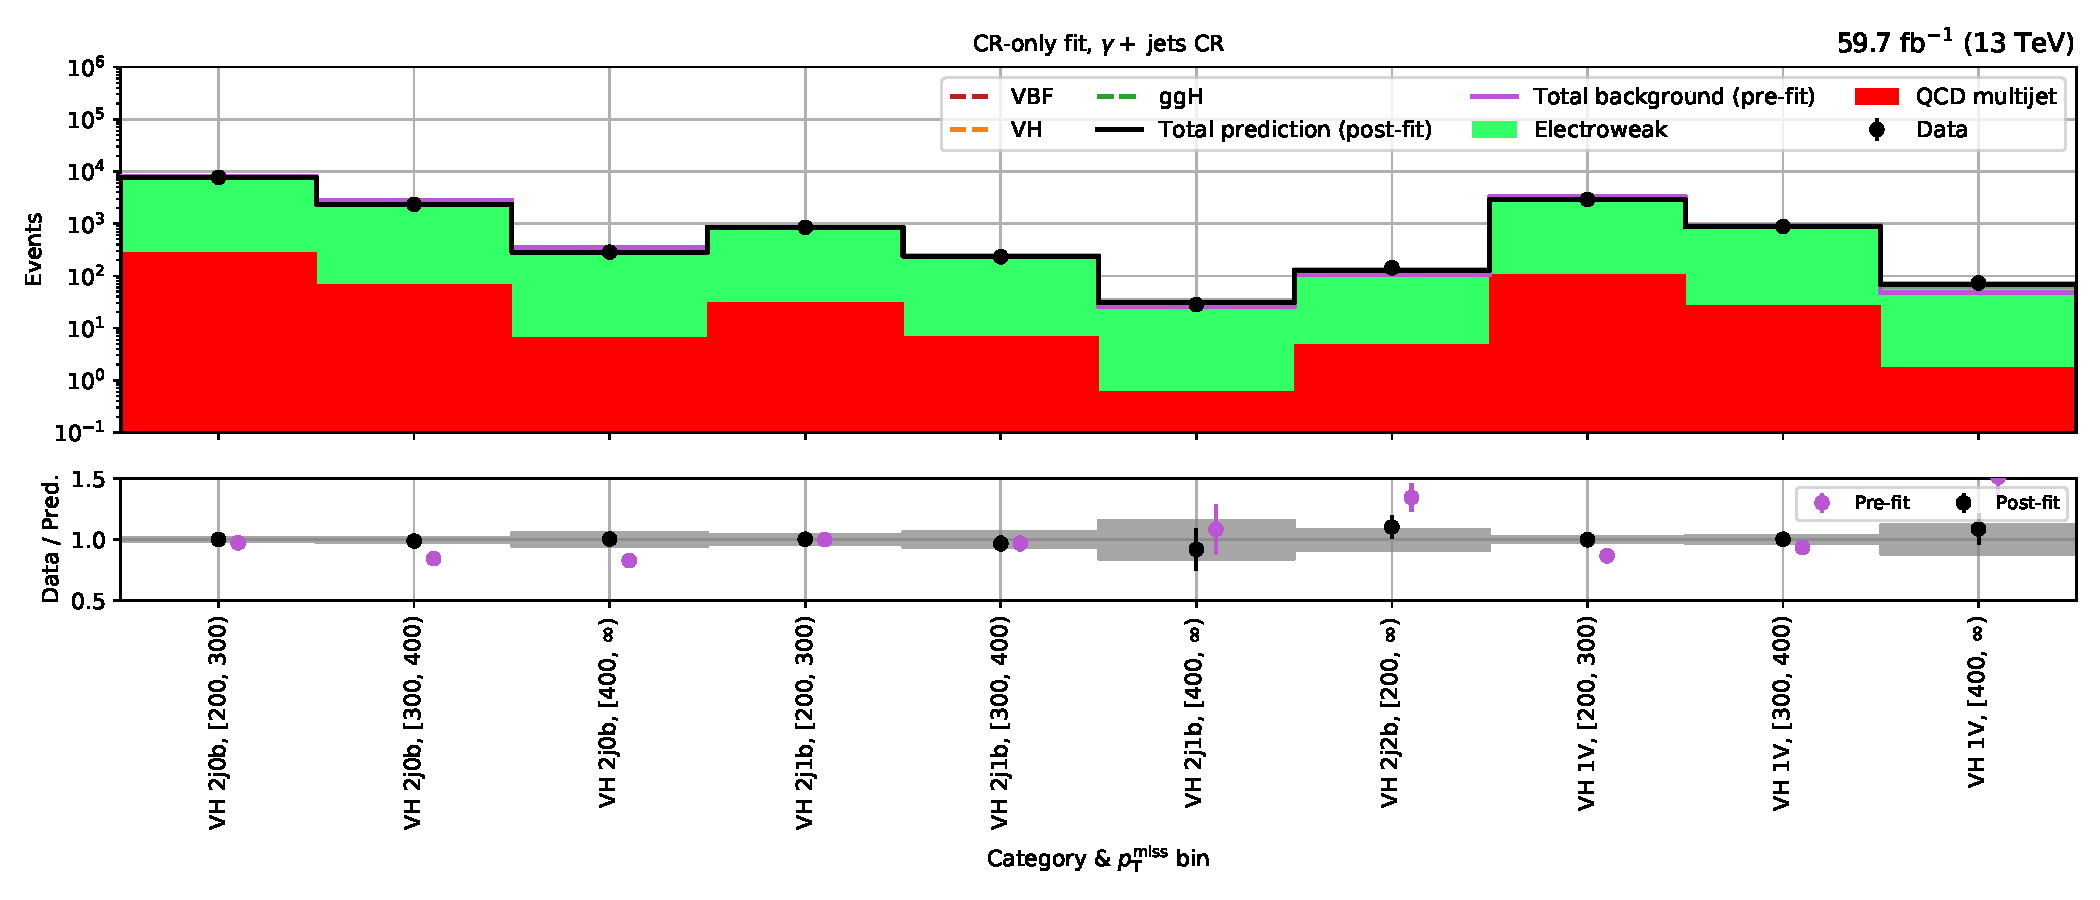
\includegraphics[width=\textwidth]{chapters/higgstoinv/figures/mountain_ranges/2018/VH/Photon_tree_fit_b-abs_values_VH_cats.pdf}
        \caption{\VH --- \singlePhotonCr \gls{CR} (2018)}
    \end{subfigure}
    \caption[Post-fit yields for each \VH category and \ptmiss bin in the lepton and photon control regions for the 2018 dataset]{Post-fit yields for each \VH category and \ptmiss bin in the lepton and photon \glspl{CR} for the 2018 dataset. The total background pre-fit and post-fit is compared to data in the lower panel of each subfigure.}
    \label{fig:htoinv_mountain_range_VH_2018_CRs}
\end{figure}

\clearpage


%=========================================================


\section{Signal region event counts after the control region-only fit}
\label{sec:yield_tables_SR_CR_only_fit}

% 2016:

\begin{table}[htbp]
    \footnotesize
    \centering
    \begin{tabular*}{\linewidth}{@{\extracolsep{\fill}}llccccr}
    \toprule
    Category & \ptmiss & Lost lepton & \ztonunu & QCD & Total SM & Data \\
    \midrule
\ttH 2Boosted & [200, 300) &    $\text{7.37} \pm \text{1.07}$ &     $\text{0} \pm \text{0}$ &  $\text{1.03} \pm \text{1.01}$ &     $\text{8.4} \pm \text{1.47}$ &    12 \\
         & [300, 400) &     $\text{2.97} \pm \text{0.5}$ &   $\text{1.26} \pm \text{0.89}$ &  $\text{0.38} \pm \text{0.62}$ &     $\text{4.61} \pm \text{1.2}$ &     1 \\
         & [400, $\infty$) &    $\text{0.61} \pm \text{0.14}$ &   $\text{1.46} \pm \text{0.75}$ &  $\text{0.18} \pm \text{0.43}$ &    $\text{2.24} \pm \text{0.87}$ &     2 \\
\ttH 1t1b & [200, 300) &    $\text{33.7} \pm \text{2.91}$ &   $\text{6.34} \pm \text{2.01}$ &  $\text{7.11} \pm \text{2.67}$ &    $\text{47.1} \pm \text{4.43}$ &    36 \\
         & [300, 400) &    $\text{25.8} \pm \text{2.35}$ &   $\text{6.61} \pm \text{1.37}$ &  $\text{2.62} \pm \text{1.62}$ &    $\text{35.0} \pm \text{3.16}$ &    45 \\
         & [400, $\infty$) &    $\text{18.9} \pm \text{1.77}$ &   $\text{7.36} \pm \text{1.82}$ &  $\text{1.27} \pm \text{1.13}$ &    $\text{27.5} \pm \text{2.78}$ &    32 \\
\ttH 1t2b & [200, 300) &    $\text{44.7} \pm \text{3.34}$ &   $\text{3.12} \pm \text{1.31}$ &  $\text{9.42} \pm \text{3.07}$ &    $\text{57.3} \pm \text{4.72}$ &    51 \\
         & [300, 400) &    $\text{41.4} \pm \text{3.13}$ &   $\text{2.68} \pm \text{1.32}$ &  $\text{3.47} \pm \text{1.86}$ &    $\text{47.5} \pm \text{3.87}$ &    40 \\
         & [400, 600) &    $\text{17.4} \pm \text{1.63}$ &   $\text{4.62} \pm \text{1.84}$ &  $\text{1.51} \pm \text{1.23}$ &    $\text{23.5} \pm \text{2.75}$ &    21 \\
         & [600, $\infty$) &    $\text{2.13} \pm \text{0.56}$ &     $\text{1.1} \pm \text{1.0}$ &  $\text{0.17} \pm \text{0.41}$ &    $\text{3.39} \pm \text{1.22}$ &     4 \\
\ttH 1W1b & [200, 300) &   $\text{375} \pm \text{15.7}$ &   $\text{46.2} \pm \text{10.8}$ &  $\text{21.6} \pm \text{4.64}$ &   $\text{443} \pm \text{19.6}$ &   396 \\
         & [300, 400) &    $\text{83.2} \pm \text{5.33}$ &   $\text{34.9} \pm \text{9.96}$ &  $\text{7.94} \pm \text{2.82}$ &   $\text{126} \pm \text{11.6}$ &   112 \\
         & [400, $\infty$) &    $\text{15.1} \pm \text{1.67}$ &   $\text{8.23} \pm \text{2.77}$ &  $\text{3.84} \pm \text{1.96}$ &    $\text{27.2} \pm \text{3.78}$ &    32 \\
\ttH 1W2b & [200, 300) &   $\text{266} \pm \text{11.0}$ &     $\text{4.0} \pm \text{2.2}$ &   $\text{14.4} \pm \text{3.8}$ &   $\text{284} \pm \text{11.8}$ &   264 \\
         & [300, 400) &    $\text{50.7} \pm \text{4.27}$ &   $\text{3.66} \pm \text{2.12}$ &  $\text{5.31} \pm \text{2.31}$ &    $\text{59.7} \pm \text{5.29}$ &    65 \\
         & [400, $\infty$) &    $\text{7.73} \pm \text{1.04}$ &    $\text{1.07} \pm \text{0.7}$ &   $\text{2.57} \pm \text{1.6}$ &    $\text{11.4} \pm \text{2.03}$ &    11 \\
\ttH 5j1b & [200, 300) &  $\text{1522} \pm \text{36.4}$ &  $\text{473} \pm \text{68.6}$ &  $\text{54.5} \pm \text{7.38}$ &  $\text{2049} \pm \text{78.1}$ &  2192 \\
         & [300, 400) &   $\text{285} \pm \text{11.8}$ &  $\text{157} \pm \text{25.5}$ &  $\text{20.1} \pm \text{4.48}$ &   $\text{461} \pm \text{28.4}$ &   516 \\
         & [400, $\infty$) &    $\text{55.1} \pm \text{4.11}$ &   $\text{92.1} \pm \text{23.0}$ &  $\text{9.69} \pm \text{3.11}$ &   $\text{157} \pm \text{23.5}$ &   189 \\
\ttH 6j1b & [200, 300) &   $\text{900} \pm \text{29.3}$ &  $\text{232} \pm \text{38.0}$ &  $\text{41.6} \pm \text{6.45}$ &  $\text{1173} \pm \text{48.4}$ &  1193 \\
         & [300, 400) &    $\text{183} \pm \text{9.5}$ &   $\text{91.8} \pm \text{19.3}$ &  $\text{15.3} \pm \text{3.91}$ &   $\text{291} \pm \text{21.9}$ &   315 \\
         & [400, $\infty$) &    $\text{51.5} \pm \text{4.15}$ &   $\text{34.6} \pm \text{12.5}$ &   $\text{7.4} \pm \text{2.72}$ &    $\text{93.5} \pm \text{13.5}$ &   114 \\
\ttH 5j2b & [200, 300) &   $\text{406} \pm \text{15.3}$ &  $\text{111} \pm \text{25.8}$ &  $\text{10.4} \pm \text{3.23}$ &   $\text{528} \pm \text{30.1}$ &   555 \\
         & [300, 400) &    $\text{47.3} \pm \text{3.73}$ &   $\text{29.0} \pm \text{11.5}$ &  $\text{3.83} \pm \text{1.96}$ &    $\text{80.2} \pm \text{12.3}$ &    87 \\
         & [400, $\infty$) &    $\text{9.38} \pm \text{1.53}$ &   $\text{16.1} \pm \text{6.95}$ &  $\text{1.85} \pm \text{1.36}$ &    $\text{27.3} \pm \text{7.25}$ &    36 \\
\ttH 6j2b & [200, 300) &   $\text{291} \pm \text{13.5}$ &   $\text{73.7} \pm \text{20.1}$ &   $\text{10.9} \pm \text{3.3}$ &   $\text{375} \pm \text{24.5}$ &   357 \\
         & [300, 400) &    $\text{45.3} \pm \text{4.11}$ &   $\text{49.4} \pm \text{13.4}$ &   $\text{4.01} \pm \text{2.0}$ &    $\text{98.7} \pm \text{14.2}$ &    76 \\
         & [400, $\infty$) &    $\text{12.4} \pm \text{1.89}$ &   $\text{4.36} \pm \text{4.16}$ &  $\text{1.94} \pm \text{1.39}$ &    $\text{18.7} \pm \text{4.77}$ &    29 \\
         \midrule
\VH 2j0b & [200, 300) &  $\text{3914} \pm \text{82.2}$ &  $\text{6497} \pm \text{247}$ &  $\text{259} \pm \text{16.1}$ &  $\text{10669} \pm \text{260}$ &  9744 \\
        & [300, 400) &   $\text{513} \pm \text{21.7}$ &   $\text{1125} \pm \text{40.9}$ &     $\text{0} \pm \text{0}$ &    $\text{1638} \pm \text{46.3}$ &  1663 \\
        & [400, $\infty$) &     $\text{48.8} \pm \text{6.0}$ &     $\text{99.5} \pm \text{8.52}$ &     $\text{0} \pm \text{0}$ &     $\text{148} \pm \text{10.4}$ &   172 \\
\VH 2j1b & [200, 300) &   $\text{545} \pm \text{20.7}$ &    $\text{571} \pm \text{34.8}$ &   $\text{1.41} \pm \text{1.19}$ &    $\text{1117} \pm \text{40.5}$ &  1060 \\
        & [300, 400) &     $\text{56.1} \pm \text{4.9}$ &    $\text{115} \pm \text{10.7}$ &     $\text{0} \pm \text{0}$ &     $\text{171} \pm \text{11.7}$ &   139 \\
        & [400, $\infty$) &    $\text{3.24} \pm \text{0.95}$ &     $\text{9.91} \pm \text{2.73}$ &     $\text{0} \pm \text{0}$ &      $\text{13.1} \pm \text{2.89}$ &    14 \\
\VH 2j2b & [200, $\infty$) &    $\text{38.4} \pm \text{4.91}$ &    $\text{160} \pm \text{18.1}$ &     $\text{0} \pm \text{0}$ &     $\text{198} \pm \text{18.7}$ &   143 \\
\VH 1V & [200, 300) &  $\text{1525} \pm \text{39.8}$ &  $\text{2836} \pm \text{120}$ &   $\text{23.5} \pm \text{4.85}$ &   $\text{4384} \pm \text{127}$ &  3899 \\
        & [300, 400) &   $\text{163} \pm \text{8.95}$ &    $\text{497} \pm \text{26.6}$ &     $\text{0} \pm \text{0}$ &     $\text{661} \pm \text{28.0}$ &   654 \\
        & [400, $\infty$) &    $\text{6.92} \pm \text{1.42}$ &     $\text{22.1} \pm \text{4.73}$ &     $\text{0} \pm \text{0}$ &      $\text{29.1} \pm \text{4.94}$ &    42 \\
        \bottomrule
    \end{tabular*}
    \caption[Event counts in the signal region after the control region-only fit to data in 2016]{Event counts in the signal region after the control region-only fit to data in 2016.}
    \label{tab:yields_SR_CR_only_2016}
\end{table}

% 2017:

\begin{table}[htbp]
    \small
    \centering
    \begin{tabular*}{\linewidth}{@{\extracolsep{\fill}}llccccr}
    \toprule
    Category & \ptmiss & Lost lepton & \ztonunu & QCD & Total SM & Data \\
    \midrule
\ttH 2Boosted & [200, 300) &    $\text{7.11} \pm \text{1.07}$ &   $\text{2.28} \pm \text{1.19}$ &   $\text{1.6} \pm \text{1.27}$ &    $\text{11.0} \pm \text{2.04}$ &     9 \\
         & [300, 400) &    $\text{2.48} \pm \text{0.36}$ &   $\text{2.23} \pm \text{0.93}$ &  $\text{0.61} \pm \text{0.78}$ &    $\text{5.32} \pm \text{1.27}$ &     6 \\
         & [400, $\infty$) &    $\text{1.17} \pm \text{0.25}$ &     $\text{1.4} \pm \text{0.5}$ &  $\text{0.32} \pm \text{0.56}$ &    $\text{2.88} \pm \text{0.79}$ &     3 \\
\ttH 1t1b & [200, 300) &    $\text{45.8} \pm \text{3.21}$ &   $\text{5.53} \pm \text{1.58}$ &   $\text{10.2} \pm \text{3.2}$ &     $\text{61.6} \pm \text{4.8}$ &    45 \\
         & [300, 400) &    $\text{38.0} \pm \text{3.09}$ &   $\text{5.96} \pm \text{1.07}$ &  $\text{3.88} \pm \text{1.97}$ &    $\text{47.8} \pm \text{3.82}$ &    52 \\
         & [400, $\infty$) &    $\text{21.2} \pm \text{1.64}$ &   $\text{8.79} \pm \text{1.87}$ &  $\text{2.02} \pm \text{1.42}$ &    $\text{32.1} \pm \text{2.86}$ &    28 \\
\ttH 1t2b & [200, 300) &    $\text{52.9} \pm \text{3.35}$ &   $\text{2.28} \pm \text{1.13}$ &  $\text{12.8} \pm \text{3.58}$ &    $\text{68.0} \pm \text{5.03}$ &    57 \\
         & [300, 400) &    $\text{45.2} \pm \text{3.23}$ &   $\text{4.12} \pm \text{1.28}$ &   $\text{4.86} \pm \text{2.2}$ &    $\text{54.1} \pm \text{4.12}$ &    38 \\
         & [400, 600) &    $\text{20.3} \pm \text{1.99}$ &   $\text{4.75} \pm \text{1.59}$ &  $\text{2.27} \pm \text{1.51}$ &    $\text{27.4} \pm \text{2.96}$ &    33 \\
         & [600, $\infty$) &     $\text{1.7} \pm \text{0.42}$ &   $\text{4.34} \pm \text{1.74}$ &   $\text{0.25} \pm \text{0.5}$ &    $\text{6.29} \pm \text{1.86}$ &     1 \\
\ttH 1W1b & [200, 300) &   $\text{385} \pm \text{15.3}$ &   $\text{32.5} \pm \text{7.73}$ &  $\text{26.8} \pm \text{5.18}$ &   $\text{445} \pm \text{17.9}$ &   410 \\
         & [300, 400) &    $\text{94.9} \pm \text{5.03}$ &   $\text{13.7} \pm \text{4.53}$ &  $\text{10.2} \pm \text{3.19}$ &   $\text{119} \pm \text{7.48}$ &   110 \\
         & [400, $\infty$) &    $\text{15.8} \pm \text{1.64}$ &   $\text{5.54} \pm \text{1.57}$ &    $\text{5.3} \pm \text{2.3}$ &    $\text{26.6} \pm \text{3.23}$ &    35 \\
\ttH 1W2b & [200, 300) &   $\text{288} \pm \text{10.4}$ &    $\text{8.06} \pm \text{3.4}$ &  $\text{18.1} \pm \text{4.26}$ &   $\text{315} \pm \text{11.8}$ &   302 \\
         & [300, 400) &    $\text{53.0} \pm \text{3.35}$ &     $\text{4.2} \pm \text{2.1}$ &  $\text{6.88} \pm \text{2.62}$ &    $\text{64.1} \pm \text{4.74}$ &    74 \\
         & [400, $\infty$) &     $\text{6.73} \pm \text{0.9}$ &   $\text{1.74} \pm \text{0.68}$ &  $\text{3.58} \pm \text{1.89}$ &     $\text{12.0} \pm \text{2.2}$ &    14 \\
\ttH 5j1b & [200, 300) &  $\text{1808} \pm \text{42.9}$ &  $\text{502} \pm \text{59.8}$ &  $\text{73.0} \pm \text{8.54}$ &  $\text{2383} \pm \text{74.1}$ &  2514 \\
         & [300, 400) &   $\text{289} \pm \text{11.9}$ &  $\text{244} \pm \text{36.4}$ &  $\text{27.7} \pm \text{5.26}$ &   $\text{561} \pm \text{38.6}$ &   540 \\
         & [400, $\infty$) &    $\text{55.2} \pm \text{3.81}$ &   $\text{82.3} \pm \text{18.3}$ &   $\text{14.4} \pm \text{3.8}$ &   $\text{152} \pm \text{19.1}$ &   152 \\
\ttH 6j1b & [200, 300) &   $\text{997} \pm \text{25.2}$ &  $\text{250} \pm \text{34.4}$ &  $\text{54.0} \pm \text{7.35}$ &  $\text{1301} \pm \text{43.2}$ &  1295 \\
         & [300, 400) &   $\text{202} \pm \text{9.39}$ &  $\text{110} \pm \text{20.8}$ &  $\text{20.5} \pm \text{4.53}$ &   $\text{332} \pm \text{23.3}$ &   343 \\
         & [400, $\infty$) &    $\text{54.0} \pm \text{4.07}$ &   $\text{40.1} \pm \text{11.9}$ &  $\text{10.7} \pm \text{3.26}$ &   $\text{105} \pm \text{13.0}$ &   121 \\
\ttH 5j2b & [200, 300) &   $\text{511} \pm \text{18.2}$ &  $\text{122} \pm \text{25.6}$ &  $\text{13.5} \pm \text{3.68}$ &   $\text{647} \pm \text{31.6}$ &   651 \\
         & [300, 400) &    $\text{45.6} \pm \text{3.51}$ &   $\text{24.9} \pm \text{10.4}$ &  $\text{5.14} \pm \text{2.27}$ &    $\text{75.6} \pm \text{11.3}$ &   106 \\
         & [400, $\infty$) &     $\text{8.78} \pm \text{1.4}$ &   $\text{22.7} \pm \text{9.85}$ &  $\text{2.67} \pm \text{1.63}$ &    $\text{34.1} \pm \text{10.1}$ &    27 \\
\ttH 6j2b & [200, 300) &   $\text{335} \pm \text{12.9}$ &   $\text{57.4} \pm \text{16.6}$ &  $\text{12.9} \pm \text{3.59}$ &   $\text{406} \pm \text{21.3}$ &   422 \\
         & [300, 400) &     $\text{51.2} \pm \text{4.4}$ &   $\text{27.7} \pm \text{11.0}$ &   $\text{4.9} \pm \text{2.21}$ &    $\text{83.8} \pm \text{12.1}$ &    87 \\
         & [400, $\infty$) &     $\text{6.86} \pm \text{1.1}$ &    $\text{4.62} \pm \text{4.0}$ &   $\text{2.55} \pm \text{1.6}$ &    $\text{14.0} \pm \text{4.45}$ &    36 \\
        \midrule
\VH 2j0b & [200, 300) &  $\text{4152} \pm \text{90.8}$ &  $\text{6090} \pm \text{208}$ &  $\text{379} \pm \text{19.5}$ &  $\text{10622} \pm \text{228}$ &  11263 \\
        & [300, 400) &   $\text{574} \pm \text{23.9}$ &    $\text{964} \pm \text{36.6}$ &     $\text{0} \pm \text{0}$ &    $\text{1538} \pm \text{43.7}$ &   1696 \\
        & [400, $\infty$) &    $\text{39.0} \pm \text{4.37}$ &    $\text{103} \pm \text{9.76}$ &     $\text{0} \pm \text{0}$ &     $\text{142} \pm \text{10.7}$ &    149 \\
\VH 2j1b & [200, 300) &   $\text{569} \pm \text{20.9}$ &    $\text{619} \pm \text{36.1}$ &   $\text{2.07} \pm \text{1.44}$ &    $\text{1190} \pm \text{41.8}$ &   1235 \\
        & [300, 400) &    $\text{56.6} \pm \text{4.26}$ &    $\text{126} \pm \text{12.1}$ &     $\text{0} \pm \text{0}$ &     $\text{183} \pm \text{12.8}$ &    190 \\
        & [400, $\infty$) &    $\text{4.27} \pm \text{1.06}$ &      $\text{9.3} \pm \text{2.42}$ &     $\text{0} \pm \text{0}$ &      $\text{13.6} \pm \text{2.64}$ &     14 \\
\VH 2j2b & [200, $\infty$) &    $\text{32.7} \pm \text{3.21}$ &    $\text{132} \pm \text{15.8}$ &     $\text{0} \pm \text{0}$ &     $\text{165} \pm \text{16.1}$ &    164 \\
\VH 1V & [200, 300) &  $\text{1349} \pm \text{42.9}$ &  $\text{2394} \pm \text{106}$ &   $\text{34.5} \pm \text{5.88}$ &   $\text{3778} \pm \text{114}$ &   4005 \\
        & [300, 400) &   $\text{169} \pm \text{8.88}$ &    $\text{511} \pm \text{30.4}$ &     $\text{0} \pm \text{0}$ &     $\text{679} \pm \text{31.7}$ &    612 \\
        & [400, $\infty$) &    $\text{6.34} \pm \text{1.14}$ &     $\text{34.8} \pm \text{5.87}$ &     $\text{0} \pm \text{0}$ &      $\text{41.2} \pm \text{5.98}$ &     50 \\
        \bottomrule
    \end{tabular*}
    \caption[Event counts in the signal region after the control region-only fit to data in 2017]{Event counts in the signal region after the control region-only fit to data in 2017.}
    \label{tab:yields_SR_CR_only_2017}
\end{table}

% 2018:

\begin{table}[htbp]
    \small
    \centering
    \begin{tabular*}{\linewidth}{@{\extracolsep{\fill}}llccccr}
    \toprule
    Category & \ptmiss & Lost lepton & \ztonunu & QCD & Total SM & Data \\
    \midrule
\ttH 2Boosted & [200, 300) &     $\text{11.2} \pm \text{1.3}$ &   $\text{1.97} \pm \text{1.11}$ &   $\text{2.2} \pm \text{1.48}$ &    $\text{15.4} \pm \text{2.26}$ &     9 \\
         & [300, 400) &    $\text{3.48} \pm \text{0.51}$ &   $\text{1.25} \pm \text{0.67}$ &  $\text{0.86} \pm \text{0.93}$ &    $\text{5.58} \pm \text{1.26}$ &     7 \\
         & [400, $\infty$) &     $\text{1.59} \pm \text{0.4}$ &   $\text{1.58} \pm \text{0.54}$ &  $\text{0.45} \pm \text{0.67}$ &    $\text{3.62} \pm \text{0.95}$ &     5 \\
\ttH 1t1b & [200, 300) &    $\text{52.4} \pm \text{3.22}$ &    $\text{7.5} \pm \text{1.55}$ &  $\text{12.4} \pm \text{3.52}$ &    $\text{72.3} \pm \text{5.02}$ &    74 \\
         & [300, 400) &    $\text{42.6} \pm \text{3.14}$ &   $\text{8.43} \pm \text{1.29}$ &   $\text{4.83} \pm \text{2.2}$ &    $\text{55.8} \pm \text{4.04}$ &    49 \\
         & [400, $\infty$) &    $\text{26.1} \pm \text{1.99}$ &   $\text{11.2} \pm \text{2.45}$ &  $\text{2.52} \pm \text{1.59}$ &    $\text{39.8} \pm \text{3.53}$ &    38 \\
\ttH 1t2b & [200, 300) &    $\text{72.2} \pm \text{4.04}$ &   $\text{7.31} \pm \text{2.21}$ &  $\text{17.9} \pm \text{4.23}$ &    $\text{97.4} \pm \text{6.25}$ &    82 \\
         & [300, 400) &    $\text{58.8} \pm \text{3.58}$ &    $\text{4.8} \pm \text{1.32}$ &  $\text{6.95} \pm \text{2.64}$ &    $\text{70.5} \pm \text{4.64}$ &    72 \\
         & [400, 600) &    $\text{27.5} \pm \text{1.96}$ &   $\text{3.67} \pm \text{1.34}$ &  $\text{3.26} \pm \text{1.81}$ &    $\text{34.4} \pm \text{2.98}$ &    42 \\
         & [600, $\infty$) &    $\text{2.27} \pm \text{0.45}$ &   $\text{3.03} \pm \text{1.25}$ &   $\text{0.36} \pm \text{0.6}$ &    $\text{5.66} \pm \text{1.45}$ &     5 \\
\ttH 1W1b & [200, 300) &   $\text{523} \pm \text{15.7}$ &   $\text{47.8} \pm \text{9.34}$ &  $\text{36.7} \pm \text{6.06}$ &   $\text{607} \pm \text{19.3}$ &   612 \\
         & [300, 400) &    $\text{114} \pm \text{4.9}$ &   $\text{15.5} \pm \text{4.11}$ &  $\text{14.3} \pm \text{3.78}$ &   $\text{144} \pm \text{7.43}$ &   149 \\
         & [400, $\infty$) &    $\text{17.7} \pm \text{1.71}$ &   $\text{6.14} \pm \text{2.15}$ &  $\text{7.45} \pm \text{2.73}$ &    $\text{31.3} \pm \text{3.87}$ &    48 \\
\ttH 1W2b & [200, 300) &   $\text{430} \pm \text{14.9}$ &   $\text{21.1} \pm \text{5.75}$ &  $\text{30.5} \pm \text{5.52}$ &   $\text{481} \pm \text{16.9}$ &   467 \\
         & [300, 400) &     $\text{84.2} \pm \text{4.9}$ &   $\text{5.88} \pm \text{2.82}$ &  $\text{11.9} \pm \text{3.44}$ &   $\text{102} \pm \text{6.62}$ &    92 \\
         & [400, $\infty$) &    $\text{14.1} \pm \text{1.33}$ &   $\text{3.62} \pm \text{1.28}$ &  $\text{6.18} \pm \text{2.49}$ &     $\text{23.9} \pm \text{3.1}$ &    27 \\
\ttH 5j1b & [200, 300) &  $\text{2043} \pm \text{37.9}$ &  $\text{672} \pm \text{66.6}$ &  $\text{93.0} \pm \text{9.65}$ &  $\text{2808} \pm \text{77.2}$ &  2989 \\
         & [300, 400) &   $\text{390} \pm \text{14.6}$ &  $\text{283} \pm \text{35.4}$ &  $\text{36.2} \pm \text{6.01}$ &   $\text{709} \pm \text{38.7}$ &   698 \\
         & [400, $\infty$) &    $\text{82.0} \pm \text{4.81}$ &  $\text{109} \pm \text{20.6}$ &  $\text{18.9} \pm \text{4.34}$ &   $\text{210} \pm \text{21.6}$ &   238 \\
\ttH 6j1b & [200, 300) &  $\text{1206} \pm \text{27.5}$ &  $\text{291} \pm \text{41.5}$ &  $\text{68.2} \pm \text{8.26}$ &  $\text{1565} \pm \text{50.4}$ &  1574 \\
         & [300, 400) &   $\text{261} \pm \text{11.1}$ &  $\text{184} \pm \text{31.1}$ &  $\text{26.5} \pm \text{5.15}$ &   $\text{472} \pm \text{33.4}$ &   445 \\
         & [400, $\infty$) &    $\text{64.4} \pm \text{4.09}$ &  $\text{109} \pm \text{22.7}$ &  $\text{13.8} \pm \text{3.72}$ &   $\text{187} \pm \text{23.3}$ &   188 \\
\ttH 5j2b & [200, 300) &   $\text{610} \pm \text{18.1}$ &  $\text{151} \pm \text{27.4}$ &  $\text{20.5} \pm \text{4.53}$ &   $\text{782} \pm \text{33.2}$ &   788 \\
         & [300, 400) &    $\text{82.4} \pm \text{4.97}$ &   $\text{58.9} \pm \text{14.4}$ &  $\text{7.99} \pm \text{2.83}$ &   $\text{149} \pm \text{15.5}$ &   159 \\
         & [400, $\infty$) &    $\text{16.7} \pm \text{1.94}$ &   $\text{26.4} \pm \text{10.8}$ &  $\text{4.17} \pm \text{2.04}$ &    $\text{47.2} \pm \text{11.1}$ &    45 \\
\ttH 6j2b & [200, 300) &   $\text{449} \pm \text{15.5}$ &  $\text{119} \pm \text{23.1}$ &  $\text{20.6} \pm \text{4.54}$ &   $\text{589} \pm \text{28.2}$ &   593 \\
         & [300, 400) &    $\text{86.6} \pm \text{6.25}$ &   $\text{41.3} \pm \text{12.6}$ &  $\text{8.02} \pm \text{2.83}$ &   $\text{136} \pm \text{14.3}$ &   144 \\
         & [400, $\infty$) &    $\text{19.1} \pm \text{2.19}$ &   $\text{23.8} \pm \text{10.1}$ &  $\text{4.19} \pm \text{2.05}$ &    $\text{47.2} \pm \text{10.5}$ &    47 \\
        \midrule
\VH 2j0b & [200, 300) &  $\text{4543} \pm \text{81.3}$ &  $\text{7000} \pm \text{217}$ &  $\text{400} \pm \text{20}$ &  $\text{11943} \pm \text{233}$ &  12086 \\
        & [300, 400) &   $\text{542} \pm \text{22.1}$ &   $\text{1149} \pm \text{37.6}$ &     $\text{0} \pm \text{0}$ &    $\text{1691} \pm \text{43.6}$ &   1827 \\
        & [400, $\infty$) &    $\text{65.0} \pm \text{6.19}$ &    $\text{124} \pm \text{10.9}$ &     $\text{0} \pm \text{0}$ &     $\text{189} \pm \text{12.6}$ &    208 \\
\VH 2j1b & [200, 300) &   $\text{707} \pm \text{23.1}$ &    $\text{685} \pm \text{36.6}$ &   $\text{2.19} \pm \text{1.48}$ &    $\text{1394} \pm \text{43.4}$ &   1519 \\
        & [300, 400) &    $\text{93.0} \pm \text{6.35}$ &    $\text{132} \pm \text{10.7}$ &     $\text{0} \pm \text{0}$ &     $\text{225} \pm \text{12.5}$ &    236 \\
        & [400, $\infty$) &    $\text{7.71} \pm \text{1.79}$ &     $\text{17.6} \pm \text{3.28}$ &     $\text{0} \pm \text{0}$ &      $\text{25.3} \pm \text{3.74}$ &     27 \\
\VH 2j2b & [200, $\infty$) &    $\text{58.1} \pm \text{5.06}$ &    $\text{216} \pm \text{21.9}$ &     $\text{0} \pm \text{0}$ &     $\text{274} \pm \text{22.5}$ &    208 \\
\VH 1V & [200, 300) &  $\text{1481} \pm \text{37}$ &   $\text{2710} \pm \text{93.8}$ &   $\text{36.4} \pm \text{6.04}$ &   $\text{4227} \pm \text{101}$ &   4815 \\
        & [300, 400) &   $\text{173} \pm \text{7.24}$ &    $\text{572} \pm \text{26.8}$ &     $\text{0} \pm \text{0}$ &     $\text{746} \pm \text{27.7}$ &    816 \\
        & [400, $\infty$) &    $\text{6.08} \pm \text{0.95}$ &     $\text{70.7} \pm \text{9.81}$ &     $\text{0} \pm \text{0}$ &      $\text{76.8} \pm \text{9.85}$ &     51 \\
        \bottomrule
    \end{tabular*}
    \caption[Event counts in the signal region after the control region-only fit to data in 2018]{Event counts in the signal region after the control region-only fit to data in 2018.}
    \label{tab:yields_SR_CR_only_2018}
\end{table}

\clearpage


%=========================================================


\section{Rate parameters from the control region-only fit}
\label{sec:rate_params_CR_only_fit}

% 2016, lost lepton prediction

\begin{table}[htbp]
    \scriptsize
    \centering
    \begin{tabular*}{\linewidth}{@{\extracolsep{\fill}}llcrcrrc}
    \toprule
    \multirow{2}{*}{Category} & \multirow{2}{*}{\ptmiss} & \multicolumn{2}{c}{\singleMuCr} & \multicolumn{2}{c}{\singleEleCr} & \multirow{2}{*}{$a_{\lostlepton}$} & \multirow{2}{*}{$N_{\lostlepton}^{\mathrm{pred.}}$}\\
     & &  MC &  Data &  MC &  Data &  & \\
\midrule
\ttH 2Boosted & [200, 300) &       62.2 &          50 &      95.1 &         99 &       0.89 &     7.37 \\
         & [300, 400) &       36.7 &          53 &      52.3 &         46 &       1.05 &     2.97 \\
         & [400, $\infty$) &       21.7 &          11 &      35.7 &         23 &       0.56 &     0.61 \\
\ttH 1t1b & [200, 300) &      153 &         131 &      93.3 &        107 &       0.93 &    33.7 \\
         & [300, 400) &      107 &          93 &      74.9 &         67 &       0.85 &    25.8 \\
         & [400, $\infty$) &       96.3 &          80 &      68.3 &         72 &       0.88 &    18.9 \\
\ttH 1t2b & [200, 300) &      176 &         140 &     116&        112 &       0.83 &    44.7 \\
         & [300, 400) &      133 &         129 &      98.1 &        103 &       0.96 &    41.4 \\
         & [400, 600) &       88.1 &          78 &      69.1 &         58 &       0.83 &    17.4 \\
         & [600, $\infty$) &       13.3 &          14 &      12.4 &          8 &       0.80 &     2.13 \\
\ttH 1W1b & [200, 300) &      815 &         625 &     588&        529 &       0.80 &   375 \\
         & [300, 400) &      260 &         219 &     204&        187 &       0.84 &    83.2 \\
         & [400, $\infty$) &       78.9 &          67 &      65.6 &         62 &       0.84 &    15.1 \\
\ttH 1W2b & [200, 300) &      636 &         460 &     461&        348 &       0.71 &   266 \\
         & [300, 400) &      196 &         145 &     148&        109 &       0.71 &    50.7 \\
         & [400, $\infty$) &       46.5 &          40 &      42.8 &         30 &       0.73 &     7.73 \\
\ttH 5j1b & [200, 300) &     2137 &        1903 &    1416&       1398 &       0.91 &  1522 \\
         & [300, 400) &      536 &         512 &     369&        377 &       0.95 &   285 \\
         & [400, $\infty$) &      173 &         156 &     127&        117 &       0.85 &    55.1 \\
\ttH 6j1b & [200, 300) &     1159 &        1073 &     750&        748 &       0.94 &   900 \\
         & [300, 400) &      349 &         328 &     245&        218 &       0.89 &   183 \\
         & [400, $\infty$) &      137&         122 &      97.6 &        114 &       0.94 &    51.5 \\
\ttH 5j2b & [200, 300) &      620 &         553 &     388&        376 &       0.89 &   406 \\
         & [300, 400) &      118 &          93 &      80.3 &         80 &       0.84 &    47.3 \\
         & [400, $\infty$) &       39.5 &          33 &      33.3 &         16 &       0.63 &     9.38 \\
\ttH 6j2b & [200, 300) &      394&         350 &     256&        241 &       0.88 &   291 \\
         & [300, 400) &       94.2 &          78 &      63.0 &         60 &       0.84 &    45.3 \\
         & [400, $\infty$) &       39.2 &          38 &      29.9 &         16 &       0.73 &    12.4 \\
\midrule
\VH 2j0b & [200, 300) &     2670&        3271 &   2140 &       2625 &       1.07 &  3914 \\
        & [300, 400) &      490&         589 &    373 &        485 &       1.11 &   513 \\
        & [400, $\infty$) &       56.5 &          79 &     42.2 &         62 &       1.32 &    48.8 \\
\VH 2j1b & [200, 300) &      573&         615 &    395 &        449 &       1.04 &   545 \\
        & [300, 400) &       91.7 &          98 &     66.7 &         70 &       1.00 &    56.1 \\
        & [400, $\infty$) &       12.9 &           6 &      7.85 &          8 &       0.64 &     3.24 \\
\VH 2j2b & [200, $\infty$) &       70.9 &          46 &     45.3 &         43 &       0.72 &    38.4 \\
\VH 1V & [200, 300) &     1698&        1616 &   1248 &       1273 &       0.89 &  1525 \\
        & [300, 400) &      278&         277 &    223 &        220 &       0.93 &   163 \\
        & [400, $\infty$) &       21.2 &          14 &     16.50 &         16 &       0.76 &     6.92 \\
\bottomrule
    \end{tabular*}
    \caption[Monte Carlo and data yields in the \singleMuCr and \singleEleCr control regions of the 2016 dataset, and corresponding rate parameter $a_{\lostlepton}$ connecting them to the signal region, for each category and \ptmiss bin]{\acrlong{mc} and data yields in the \singleMuCr and \singleEleCr \glspl{CR} of the 2016 dataset, and corresponding rate parameter $a_{\lostlepton}$ connecting them to the signal region, for each category and \ptmiss bin. The predicted lost lepton background in the signal region $N_{\lostlepton}^{\mathrm{pred.}}$ is also given.}
    \label{tab:htoinv_rate_params_2016_lost_lep}
\end{table}

% 2016, Z->inv prediction

\begin{table}[htbp]
    \centering
    \small
    \begin{tabular*}{\linewidth}{@{\extracolsep{\fill}}llcrcrcrrc}
    \toprule
    \multirow{2}{*}{Category} & \multirow{2}{*}{\ptmiss} & \multicolumn{2}{c}{\doubleMuCr} & \multicolumn{2}{c}{\doubleEleCr} & \multicolumn{2}{c}{\singlePhotonCr} & \multirow{2}{*}{$a_{\ztonunu}$} & \multirow{2}{*}{$N_{\ztonunu}^{\mathrm{pred.}}$} \\
     & &  MC &  Data &  MC &  Data & MC & Data & &  \\
    \midrule
\ttH 2Boosted & [200, 300) &       0.90 &           0 &     0.85 &         0 &         --- & --- &       0.00 &     0.00 \\
    & [300, 400) &       0.88 &           1 &     0.53 &         1 &         --- & --- &       1.31 &     1.26 \\
    & [400, $\infty$) &       1.76 &           1 &     1.07 &         3 &         --- & --- &       1.24 &     1.46 \\
\ttH 1t1b & [200, 300) &       7.28 &           9 &     3.72 &         4 &         --- & --- &       1.19 &     6.34 \\
    & [300, 400) &      10.3 &          16 &     4.73 &         4 &         --- & --- &       1.28 &     6.61 \\
    & [400, $\infty$) &      11.4 &           8 &     5.23 &         9 &         --- & --- &       0.88 &     7.36 \\
\ttH 1t2b & [200, 300) &       1.97 &           3 &     1.87 &         2 &         --- & --- &       1.27 &     3.12 \\
    & [300, 400) &       2.91 &           2 &     1.55 &         2 &         --- & --- &       0.85 &     2.68 \\
    & [400, 600) &       2.53 &           4 &     2.04 &         3 &         --- & --- &       1.35 &     4.62 \\
    & [600, $\infty$) &       0.69 &           0 &     0.45 &         1 &         --- & --- &       0.70 &     1.10 \\
\ttH 1W1b & [200, 300) &       9.72 &          10 &    10.7 &        12 &         --- & --- &       1.06 &    46.2 \\
    & [300, 400) &       3.13 &           8 &     4.24 &         8 &         --- & --- &       2.03 &    34.9 \\
    & [400, $\infty$) &       2.93 &           4 &    10.1 &         8 &         --- & --- &       0.74 &     8.23 \\
\ttH 1W2b & [200, 300) &       2.77 &           1 &     3.09 &         2 &         --- & --- &       0.50 &     4.00 \\
    & [300, 400) &       1.02 &           3 &     1.87 &         0 &         --- & --- &       0.96 &     3.66 \\
    & [400, $\infty$) &       1.36 &           0 &     2.20 &         2 &         --- & --- &       0.46 &     1.07 \\
\ttH 5j1b & [200, 300) &      64.1 &          60 &    45.1 &        40 &         --- & --- &       0.96 &   473 \\
    & [300, 400) &      29.3 &          22 &    19.5 &        18 &         --- & --- &       0.80 &   157 \\
    & [400, $\infty$) &      14.1 &          13 &     9.86 &         9 &         --- & --- &       0.82 &    92.1 \\
\ttH 6j1b & [200, 300) &      26.9 &          33 &    19.6 &        17 &         --- & --- &       1.12 &   232 \\
    & [300, 400) &      14.7 &          11 &     9.79 &        12 &         --- & --- &       0.91 &    91.8 \\
    & [400, $\infty$) &       8.72 &           5 &     5.58 &         3 &         --- & --- &       0.49 &    34.6 \\
\ttH 5j2b & [200, 300) &      13.5 &          16 &     9.05 &         8 &         --- & --- &       1.08 &   111 \\
    & [300, 400) &       5.31 &           3 &     4.02 &         4 &         --- & --- &       0.73 &    29.0 \\
    & [400, $\infty$) &       3.05 &           5 &     2.75 &         0 &         --- & --- &       0.77 &    16.1 \\
\ttH 6j2b & [200, 300) &       7.90 &           9 &     5.48 &         7 &         --- & --- &       1.21 &    73.7 \\
    & [300, 400) &       4.03 &           5 &     2.69 &         7 &         --- & --- &       1.69 &    49.4 \\
    & [400, $\infty$) &       1.95 &           1 &     1.72 &         0 &         --- & --- &       0.24 &     4.36 \\
    \midrule
\VH 2j0b & [200, 300) &     486 &         566 &   328 &       359 &      5236&         5013 &       0.93 &  6497 \\
    & [300, 400) &      97.9 &         129 &    66.8 &        83 &      1871&         1729 &       0.92 &  1125 \\
    & [400, $\infty$) &      11 &          15 &     7.25 &         8 &       222&          174 &       0.79 &    99.5 \\
\VH 2j1b & [200, 300) &      49.9 &          51 &    36.3 &        46 &       418&          450 &       1.02 &   571 \\
    & [300, 400) &      11.7 &          13 &     7.61 &        11 &       136&          147 &       1.06 &   115 \\
    & [400, $\infty$) &       1.43 &           0 &     1.36 &         2 &        16.9 &           15 &       0.83 &     9.91 \\
\VH 2j2b & [200, $\infty$) &      11 &          14 &     8.59 &         8 &        52.6 &           81 &       1.35 &   160 \\
\VH 1V & [200, 300) &     219 &         217 &   140 &       154 &      2030&         1950 &       0.92 &  2836 \\
& [300, 400) &      38.3 &          45 &    28.7 &        28 &       571&          566 &       0.96 &   497 \\
& [400, $\infty$) &       3.04 &           1 &     1.79 &         1 &        26.4 &           21 &       0.71 &    22.1 \\
\bottomrule
\end{tabular*}
\caption[Monte Carlo and data yields in the \doubleMuCr, \doubleEleCr, and \singlePhotonCr control regions of the 2016 dataset, and corresponding rate parameter $a_{\ztonunu}$ connecting them to the signal region, for each category and \ptmiss bin]{\acrlong{mc} and data yields in the \doubleMuCr, \doubleEleCr, and \singlePhotonCr \glspl{CR} of the 2016 dataset, and corresponding rate parameter $a_{\ztonunu}$ connecting them to the signal region, for each category and \ptmiss bin. The predicted invisible \PZ background in the signal region $N_{\ztonunu}^{\mathrm{pred.}}$ is also given.}
\label{tab:htoinv_rate_params_2016_zinv}
\end{table}

% 2017, lost lepton prediction

\begin{table}[htbp]
    \small
    \centering
    \begin{tabular*}{\linewidth}{@{\extracolsep{\fill}}llcrcrrc}
    \toprule
    \multirow{2}{*}{Category} & \multirow{2}{*}{\ptmiss} & \multicolumn{2}{c}{\singleMuCr} & \multicolumn{2}{c}{\singleEleCr} & \multirow{2}{*}{$a_{\lostlepton}$} & \multirow{2}{*}{$N_{\lostlepton}^{\mathrm{pred.}}$}\\
     & &  MC &  Data &  MC &  Data &  & \\
\midrule
\ttH 2Boosted & [200, 300) &       59.1 &          72 &     93.8 &         99 &       1.13 &     7.11 \\
         & [300, 400) &       38.8 &          46 &     61.5 &         74 &       1.20 &     2.48 \\
         & [400, $\infty$) &       26.0 &          36 &     38.3 &         41 &       1.17 &     1.17 \\
\ttH 1t1b & [200, 300) &      155 &         174 &    111 &        117 &       1.12 &    45.8 \\
         & [300, 400) &      119 &         128 &     90 &         95 &       1.08 &    38.0 \\
         & [400, $\infty$) &       99.9 &         105 &     82.1 &         74 &       0.98 &    21.2 \\
\ttH 1t2b & [200, 300) &      178 &         168 &    124 &        129 &       0.99 &    52.90 \\
         & [300, 400) &      138 &         138 &    105 &        125 &       1.08 &    45.20 \\
         & [400, 600) &       88.1 &          94 &     69.4 &         72 &       1.05 &    20.3 \\
         & [600, $\infty$) &       11.7 &          13 &      8.94 &          7 &       0.94 &     1.70 \\
\ttH 1W1b & [200, 300) &      731 &         683 &    562 &        520 &       0.97 &   385 \\
         & [300, 400) &      242 &         248 &    188 &        186 &       1.04 &    94.9 \\
         & [400, $\infty$) &       80.9 &          83 &     64.7 &         64 &       1.04 &    15.8 \\
\ttH 1W2b & [200, 300) &      592 &         534 &    431 &        360 &       0.90 &   288 \\
         & [300, 400) &      176 &         141 &    137 &        112 &       0.82 &    53.0 \\
         & [400, $\infty$) &       50.7 &          28 &     40.7 &         36 &       0.72 &     6.73 \\
\ttH 5j1b & [200, 300) &     2143 &        2317 &   1410 &       1611 &       1.12 &  1808 \\
         & [300, 400) &      536 &         550 &    377 &        404 &       1.05 &   289 \\
         & [400, $\infty$) &      166 &         184 &    125 &        112 &       1.02 &    55.2 \\
\ttH 6j1b & [200, 300) &     1088 &        1205 &    738 &        804 &       1.13 &   997 \\
         & [300, 400) &      320 &         357 &    232 &        262 &       1.14 &   202 \\
         & [400, $\infty$) &      121 &         153 &     85.2 &        104 &       1.26 &    54.0 \\
\ttH 5j2b & [200, 300) &      592 &         690 &    411 &        423 &       1.11 &   511 \\
         & [300, 400) &      111 &          99 &     88.2 &         73 &       0.85 &    45.6 \\
         & [400, $\infty$) &       34.4 &          22 &     27.7 &         34 &       0.89 &     8.78 \\
\ttH 6j2b & [200, 300) &      381 &         386 &    264 &        290 &       1.05 &   335 \\
         & [300, 400) &       86.5 &          99 &     61.6 &         59 &       1.06 &    51.2 \\
         & [400, $\infty$) &       32.1 &          16 &     24.2 &         21 &       0.65 &     6.86 \\
\midrule
\VH 2j0b & [200, 300) &    3269 &        3687 &   2352 &       2894 &       1.21 &  4152 \\
        & [300, 400) &     530 &         653 &    411 &        529 &       1.28 &   574 \\
        & [400, $\infty$) &      55.9 &          70 &     53.8 &         60 &       1.19 &    39.0 \\
\VH 2j1b & [200, 300) &     593 &         706 &    452 &        517 &       1.18 &   569 \\
        & [300, 400) &      96.7 &          96 &     70.0 &         77 &       1.03 &    56.6 \\
        & [400, $\infty$) &       8.75 &          12 &      8.05 &          6 &       1.03 &     4.27 \\
\VH 2j2b & [200, $\infty$) &      71.7 &          57 &     57.2 &         46 &       0.79 &    32.7 \\
\VH 1V & [200, 300) &    1989 &        1680 &   1392 &       1157 &       0.88 &  1349 \\
        & [300, 400) &     420 &         322 &    327 &        252 &       0.78 &   169 \\
        & [400, $\infty$) &      35.2 &          24 &     28.1 &         20 &       0.70 &     6.34 \\
\bottomrule
    \end{tabular*}
    \caption[Monte Carlo and data yields in the \singleMuCr and \singleEleCr control regions of the 2017 dataset, and corresponding rate parameter $a_{\lostlepton}$ connecting them to the signal region, for each category and \ptmiss bin]{\acrlong{mc} and data yields in the \singleMuCr and \singleEleCr \glspl{CR} of the 2017 dataset, and corresponding rate parameter $a_{\lostlepton}$ connecting them to the signal region, for each category and \ptmiss bin. The predicted lost lepton background in the signal region $N_{\lostlepton}^{\mathrm{pred.}}$ is also given.}
    \label{tab:htoinv_rate_params_2017_lost_lep}
\end{table}

% 2017, Z->inv prediction

\begin{table}[htbp]
    \centering
    \small
    \begin{tabular*}{\linewidth}{@{\extracolsep{\fill}}llcrcrcrrc}
    \toprule
    \multirow{2}{*}{Category} & \multirow{2}{*}{\ptmiss} & \multicolumn{2}{c}{\doubleMuCr} & \multicolumn{2}{c}{\doubleEleCr} & \multicolumn{2}{c}{\singlePhotonCr} & \multirow{2}{*}{$a_{\ztonunu}$} & \multirow{2}{*}{$N_{\ztonunu}^{\mathrm{pred.}}$} \\
     & &  MC &  Data &  MC &  Data & MC & Data & &  \\
    \midrule
\ttH 2Boosted & [200, 300) &       1.09 &           1 &     1.38 &         2 &         --- & --- &       1.34 &     2.28 \\
    & [300, 400) &       1.26 &           2 &     1.42 &         3 &         --- & --- &       1.83 &     2.23 \\
    & [400, $\infty$) &       2.16 &           6 &     3.34 &         3 &         --- & --- &       1.61 &     1.40 \\
\ttH 1t1b & [200, 300) &       6.77 &           9 &     4.64 &         5 &         --- & --- &       1.21 &     5.53 \\
    & [300, 400) &      13.0 &          26 &     5.65 &         7 &         --- & --- &       1.73 &     5.96 \\
    & [400, $\infty$) &      21.2 &          38 &     8.08 &         6 &         --- & --- &       1.42 &     8.79 \\
\ttH 1t2b & [200, 300) &       2.64 &           2 &     2.11 &         2 &         --- & --- &       0.87 &     2.28 \\
    & [300, 400) &       3.24 &           6 &     1.75 &         4 &         --- & --- &       2.01 &     4.12 \\
    & [400, 600) &       3.42 &           6 &     2.43 &         4 &         --- & --- &       1.65 &     4.75 \\
    & [600, $\infty$) &       1.03 &           4 &     0.38 &         3 &         --- & --- &       4.63 &     4.34 \\
\ttH 1W1b & [200, 300) &       8.43 &          13 &    11.4 &        12 &         --- & --- &       1.31 &    32.5 \\
    & [300, 400) &       2.83 &           5 &     7.71 &         5 &         --- & --- &       0.99 &    13.7 \\
    & [400, $\infty$) &       5.39 &           5 &    37.9 &        26 &         --- & --- &       0.70 &     5.54 \\
\ttH 1W2b & [200, 300) &       2.35 &           2 &     4.55 &         4 &         --- & --- &       0.89 &     8.06 \\
    & [300, 400) &       1.05 &           1 &     2.36 &         3 &         --- & --- &       1.22 &     4.20 \\
    & [400, $\infty$) &       1.64 &           4 &     6.47 &         6 &         --- & --- &       1.23 &     1.74 \\
\ttH 5j1b & [200, 300) &      71.0 &          83 &    44.3 &        46 &         --- & --- &       1.15 &   502 \\
    & [300, 400) &      25.2 &          34 &    18.8 &        32 &         --- & --- &       1.52 &   244 \\
    & [400, $\infty$) &      11.1 &          16 &     8.08 &         5 &         --- & --- &       1.07 &    82.3 \\
\ttH 6j1b & [200, 300) &      25.0 &          37 &    17.4 &        29 &         --- & --- &       1.60 &   250 \\
    & [300, 400) &      12.0 &          21 &     8.57 &        12 &         --- & --- &       1.62 &   110 \\
    & [400, $\infty$) &       5.94 &           5 &     4.70 &         6 &         --- & --- &       1.05 &    40.1 \\
\ttH 5j2b & [200, 300) &      15.5 &          19 &    12.4 &        15 &         --- & --- &       1.27 &   122 \\
    & [300, 400) &       5.85 &           4 &     3.93 &         3 &         --- & --- &       0.72 &    24.9 \\
    & [400, $\infty$) &       1.94 &           1 &     1.40 &         4 &         --- & --- &       1.46 &    22.7 \\
\ttH 6j2b & [200, 300) &       7.57 &          11 &     5.97 &         5 &         --- & --- &       1.25 &    57.4 \\
    & [300, 400) &       3.20 &           4 &     2.07 &         3 &         --- & --- &       1.31 &    27.7 \\
    & [400, $\infty$) &       1.02 &           1 &     0.98 &         0 &         --- & --- &       0.48 &     4.62 \\
    \midrule
\VH 2j0b & [200, 300) &     621 &         680 &   428 &       435 &      5025 &         5662 &       1.04 &   6090 \\
    & [300, 400) &     120 &         106 &    82.9 &        78 &      1771 &         1824 &       0.93 &    964 \\
    & [400, $\infty$) &      14.9 &          11 &     8.89 &         6 &       217 &          214 &       0.88 &    103 \\
\VH 2j1b & [200, 300) &      67.0 &          71 &    42.1 &        34 &       391 &          578 &       1.22 &    619 \\
    & [300, 400) &      12.1 &          13 &     7.02 &        11 &       114 &          168 &       1.37 &    126 \\
    & [400, $\infty$) &       1.96 &           4 &     1.47 &         1 &        13.3 &           14 &       1.03 &      9.3 \\
\VH 2j2b & [200, $\infty$) &      16.3 &          14 &    11.1 &         6 &        50.3 &           69 &       1.03 &    132 \\
\VH 1V & [200, 300) &     265 &         223 &   184 &       146 &      1935 &         2048 &       0.97 &   2394 \\
& [300, 400) &      47.3 &          48 &    34.3 &        36 &       525 &          618 &       1.08 &    511 \\
& [400, $\infty$) &       3.53 &           8 &     2.15 &         1 &        32.8 &           39 &       1.17 &     34.8 \\
\bottomrule
\end{tabular*}
\caption[Monte Carlo and data yields in the \doubleMuCr, \doubleEleCr, and \singlePhotonCr control regions of the 2017 dataset, and corresponding rate parameter $a_{\ztonunu}$ connecting them to the signal region, for each category and \ptmiss bin]{\acrlong{mc} and data yields in the \doubleMuCr, \doubleEleCr, and \singlePhotonCr \glspl{CR} of the 2017 dataset, and corresponding rate parameter $a_{\ztonunu}$ connecting them to the signal region, for each category and \ptmiss bin. The predicted invisible \PZ background in the signal region $N_{\ztonunu}^{\mathrm{pred.}}$ is also given.}
\label{tab:htoinv_rate_params_2017_zinv}
\end{table}

% 2018, lost lepton prediction

\begin{table}[htbp]
    \small
    \centering
    \begin{tabular*}{\linewidth}{@{\extracolsep{\fill}}llcrcrrc}
    \toprule
    \multirow{2}{*}{Category} & \multirow{2}{*}{\ptmiss} & \multicolumn{2}{c}{\singleMuCr} & \multicolumn{2}{c}{\singleEleCr} & \multirow{2}{*}{$a_{\lostlepton}$} & \multirow{2}{*}{$N_{\lostlepton}^{\mathrm{pred.}}$}\\
     & &  MC &  Data &  MC &  Data &  & \\
\midrule
\ttH 2Boosted & [200, 300) &      111 &         121 &     177 &        166 &       1.01 &    11.2 \\
         & [300, 400) &       74.9 &          74 &     120 &         85 &       0.82 &     3.48 \\
         & [400, $\infty$) &       51.1 &          38 &      73.1 &         66 &       0.81 &     1.59 \\
\ttH 1t1b & [200, 300) &      249 &         230 &     183 &        159 &       0.93 &    52.4 \\
         & [300, 400) &      200 &         172 &     143 &        124 &       0.85 &    42.6 \\
         & [400, $\infty$) &      172 &         141 &     127 &        101 &       0.80 &    26.1 \\
\ttH 1t2b & [200, 300) &      329 &         290 &     243 &        199 &       0.87 &    72.2 \\
         & [300, 400) &      261 &         243 &     203 &        151 &       0.83 &    58.8 \\
         & [400, 600) &      177 &         142 &     138 &        103 &       0.77 &    27.5 \\
         & [600, $\infty$) &       21.6 &          21 &      18.6 &         10 &       0.73 &     2.27 \\
\ttH 1W1b & [200, 300) &     1193 &        1051 &     958 &        837 &       0.93 &   523 \\
         & [300, 400) &      404 &         343 &     327 &        274 &       0.86 &   114 \\
         & [400, $\infty$) &      143 &         106 &     122 &         85 &       0.73 &    17.7 \\
\ttH 1W2b & [200, 300) &     1036 &         839 &     823 &        699 &       0.85 &   430 \\
         & [300, 400) &      327 &         248 &     263 &        207 &       0.77 &    84.2 \\
         & [400, $\infty$) &       93.9 &          79 &      74.7 &         74 &       0.89 &    14.1 \\
\ttH 5j1b & [200, 300) &     3300 &        3030 &    2414 &       2191 &       0.95 &  2043 \\
         & [300, 400) &      838 &         851 &     620 &        591 &       1.02 &   390 \\
         & [400, $\infty$) &      275 &         268 &     208 &        199 &       0.96 &    82 \\
\ttH 6j1b & [200, 300) &     1726 &        1667 &    1242 &       1108 &       0.98 &  1206 \\
         & [300, 400) &      521 &         515 &     365 &        354 &       1.01 &   261 \\
         & [400, $\infty$) &      208 &         225 &     150 &        138 &       1.03 &    64.4 \\
\ttH 5j2b & [200, 300) &     1053 &         953 &     763 &        681 &       0.90 &   610 \\
         & [300, 400) &      205 &         187 &     157 &        143 &       0.88 &    82.4 \\
         & [400, $\infty$) &       56.4 &          71 &      48.3 &         32 &       0.95 &    16.7 \\
\ttH 6j2b & [200, 300) &      711 &         618 &     488 &        447 &       0.88 &   449 \\
         & [300, 400) &      159 &         171 &     118 &        109 &       0.99 &    86.6 \\
         & [400, $\infty$) &       66.4 &          61 &      45.5 &         43 &       0.89 &    19.1 \\
\midrule
\VH 2j0b & [200, 300) &     4604 &        4563 &    3673 &       3907 &       1.19 &  4543 \\
        & [300, 400) &      788 &         818 &     626 &        647 &       1.17 &   542 \\
        & [400, $\infty$) &       85.2 &         110 &      83.7 &         88 &       1.23 &    65 \\
\VH 2j1b & [200, 300) &      897 &         947 &     719 &        767 &       1.10 &   707 \\
        & [300, 400) &      133 &         158 &      93.6 &        137 &       1.31 &    93 \\
        & [400, $\infty$) &       15.4 &          17 &      11.2 &         12 &       1.07 &     7.71 \\
\VH 2j2b & [200, $\infty$) &      124 &         126 &     116 &         89 &       0.94 &    58.1 \\
\VH 1V & [200, 300) &     2747 &        2183 &    2208 &       1748 &       0.89 &  1481 \\
        & [300, 400) &      622 &         423 &     488 &        333 &       0.73 &   173 \\
        & [400, $\infty$) &       48.6 &          22 &      43.4 &         20 &       0.47 &     6.08 \\
\bottomrule
    \end{tabular*}
    \caption[Monte Carlo and data yields in the \singleMuCr and \singleEleCr control regions of the 2018 dataset, and corresponding rate parameter $a_{\lostlepton}$ connecting them to the signal region, for each category and \ptmiss bin]{\acrlong{mc} and data yields in the \singleMuCr and \singleEleCr \glspl{CR} of the 2018 dataset, and corresponding rate parameter $a_{\lostlepton}$ connecting them to the signal region, for each category and \ptmiss bin. The predicted lost lepton background in the signal region $N_{\lostlepton}^{\mathrm{pred.}}$ is also given.}
    \label{tab:htoinv_rate_params_2018_lost_lep}
\end{table}

% 2018, Z->inv prediction

\begin{table}[htbp]
    \centering
    \small
    \begin{tabular*}{\linewidth}{@{\extracolsep{\fill}}llcrcrcrrc}
    \toprule
    \multirow{2}{*}{Category} & \multirow{2}{*}{\ptmiss} & \multicolumn{2}{c}{\doubleMuCr} & \multicolumn{2}{c}{\doubleEleCr} & \multicolumn{2}{c}{\singlePhotonCr} & \multirow{2}{*}{$a_{\ztonunu}$} & \multirow{2}{*}{$N_{\ztonunu}^{\mathrm{pred.}}$} \\

     & &  MC &  Data &  MC &  Data & MC & Data & &  \\
    \midrule
    \ttH 2Boosted & [200, 300) &       1.86 &           2 &     1.72 &         1 &         --- & --- &       0.87 &     1.97 \\
    & [300, 400) &       2.75 &           3 &     1.39 &         0 &         --- & --- &       0.77 &     1.25 \\
    & [400, $\infty$) &       4.25 &           5 &     7.23 &         6 &         --- & --- &       0.85 &     1.58 \\
    \ttH 1t1b & [200, 300) &      14.9 &          15 &     9.94 &        14 &         --- & --- &       1.23 &     7.50 \\
    & [300, 400) &      23.0 &          21 &    10.8 &        23 &         --- & --- &       1.30 &     8.43 \\
    & [400, $\infty$) &      34.4 &          40 &    13.8 &        14 &         --- & --- &       1.09 &    11.2 \\
\ttH 1t2b & [200, 300) &       4.41 &           7 &     3.85 &         8 &         --- & --- &       1.81 &     7.31 \\
    & [300, 400) &       5.50 &           7 &     4.41 &         6 &         --- & --- &       1.31 &     4.80 \\
    & [400, 600) &       6.69 &           7 &     5.23 &         2 &         --- & --- &       0.71 &     3.67 \\
    & [600, $\infty$) &       2.33 &           6 &     1.49 &         2 &         --- & --- &       2.03 &     3.03 \\
\ttH 1W1b & [200, 300) &      15.6&          19 &    26.2 &        19 &         --- & --- &       1.01 &    47.8 \\
    & [300, 400) &       6.29 &           7 &    15.0 &         8 &         --- & --- &       0.80 &    15.5 \\
    & [400, $\infty$) &       8.89 &           6 &    78.9 &        36 &         --- & --- &       0.50 &     6.14 \\
\ttH 1W2b & [200, 300) &       4.62 &          10 &     6.37 &         5 &         --- & --- &       1.37 &    21.1 \\
    & [300, 400) &       2.69 &           1 &     5.02 &         4 &         --- & --- &       0.60 &     5.88 \\
    & [400, $\infty$) &       2.89 &           4 &    13.2 &        14 &         --- & --- &       1.16 &     3.62 \\
\ttH 5j1b & [200, 300) &     118 &         118 &    89.1 &        80 &         --- & --- &       1.09 &   672 \\
    & [300, 400) &      48.1 &          53 &    35.9 &        34 &         --- & --- &       1.08 &   283 \\
    & [400, $\infty$) &      19.5 &          16 &    15.4 &        16 &         --- & --- &       0.92 &   109 \\
    \ttH 6j1b & [200, 300) &      42.2 &          46 &    34.4 &        36 &         --- & --- &       1.21 &   291 \\
    & [300, 400) &      20.2 &          32 &    15.4 &        24 &         --- & --- &       1.72 &   184 \\
    & [400, $\infty$) &      10.6 &          17 &     7.06 &        11 &         --- & --- &       1.75 &   109 \\
\ttH 5j2b & [200, 300) &      29.4 &          32 &    22.6 &        15 &         --- & --- &       1.00 &   151 \\
    & [300, 400) &      11.9 &          12 &     6.36 &         7 &         --- & --- &       1.08 &    58.9 \\
    & [400, $\infty$) &       3.63 &           5 &     2.95 &         2 &         --- & --- &       1.11 &    26.4 \\
\ttH 6j2b & [200, 300) &      12.1 &          19 &     9.83 &        14 &         --- & --- &       1.46 &   119 \\
    & [300, 400) &       6.05 &           6 &     4.17 &         6 &         --- & --- &       1.15 &    41.3 \\
    & [400, $\infty$) &       2.35 &           2 &     2.03 &         4 &         --- & --- &       1.38 &    23.8 \\
    \midrule
\VH 2j0b & [200, 300) &     826 &         794 &   615 &       549 &      7636 &         7707 &       1.13 &   7000 \\
    & [300, 400) &     171 &         174 &   128 &       115 &      2695 &         2332 &       0.92 &   1149 \\
    & [400, $\infty$) &      18.0 &          18 &    13.4 &         9 &       337 &          284 &       0.88 &    124 \\
\VH 2j1b & [200, 300) &      83.5 &          86 &    81.4 &        70 &       817 &          847 &       1.06 &    685 \\
    & [300, 400) &      18.8 &          25 &    12.6 &        15 &       231 &          231 &       1.08 &    132 \\
    & [400, $\infty$) &       3.40 &           9 &     2.24 &         1 &        25.2 &           28 &       1.25 &     17.6 \\
\VH 2j2b & [200, $\infty$) &      25.9 &          25 &    13.6 &         8 &       101 &          142 &       1.22 &    216 \\
\VH 1V & [200, 300) &     356 &         337 &   271 &       197 &      3212 &         2876 &       1.06 &   2710 \\
& [300, 400) &      71.2 &          73 &    50.8 &        39 &       911 &          876 &       1.09 &    572 \\
& [400, $\infty$) &       4.94 &           6 &     4.57 &         2 &        46.5 &           73 &       1.53 &     70.7 \\
\bottomrule
\end{tabular*}
\caption[Monte Carlo and data yields in the \doubleMuCr, \doubleEleCr, and \singlePhotonCr control regions of the 2018 dataset, and corresponding rate parameter $a_{\ztonunu}$ connecting them to the signal region, for each category and \ptmiss bin]{\acrlong{mc} and data yields in the \doubleMuCr, \doubleEleCr, and \singlePhotonCr \glspl{CR} of the 2018 dataset, and corresponding rate parameter $a_{\ztonunu}$ connecting them to the signal region, for each category and \ptmiss bin. The predicted invisible \PZ background in the signal region $N_{\ztonunu}^{\mathrm{pred.}}$ is also given.}
\label{tab:htoinv_rate_params_2018_zinv}
\end{table}

\clearpage


%=========================================================


\section{Background-only fits to the \texorpdfstring{\ttH}{ttH} categories}
\label{sec:B_only_fit_plots_ttH_SR}

\begin{figure}[htbp]
    \centering
    \begin{subfigure}[b]{0.9\textwidth}
        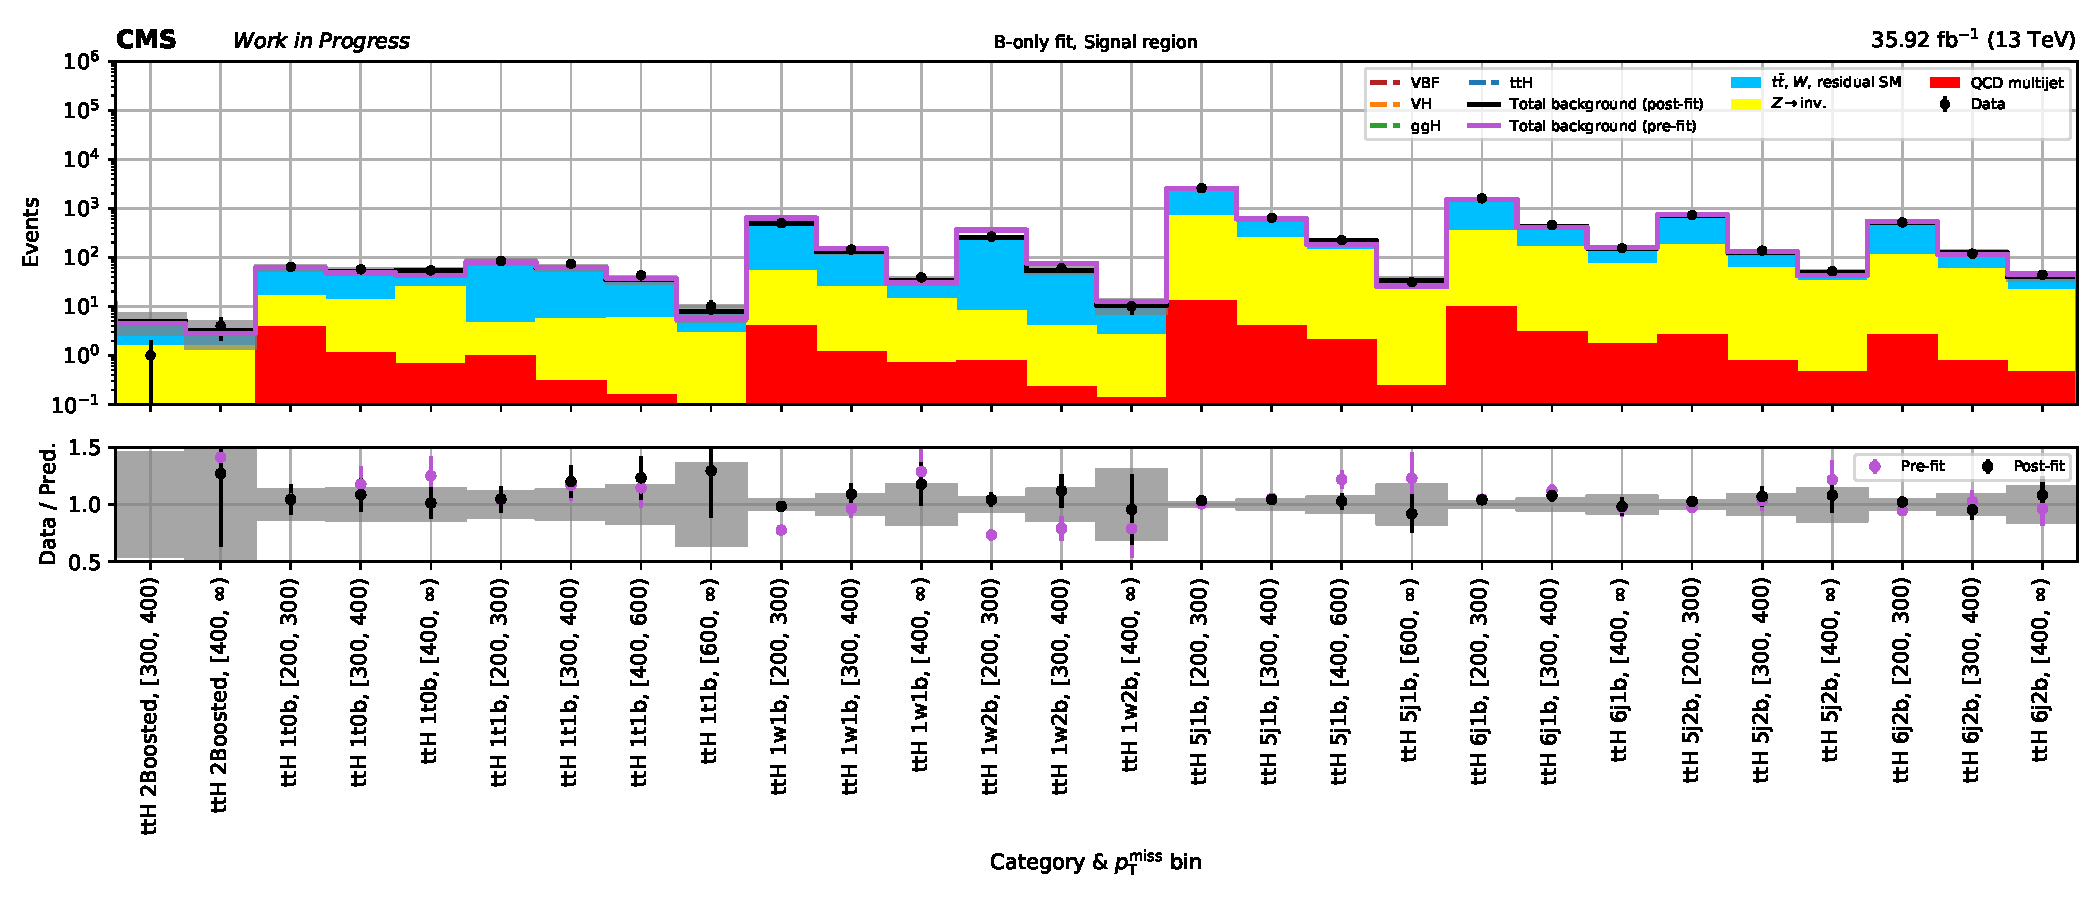
\includegraphics[width=\textwidth]{chapters/higgstoinv/figures/mountain_ranges/2016/ttH/SR_tree_fit_b-abs_values_ttH_cats.pdf}
        \caption{\ttH --- 2016}
    \end{subfigure}

    \begin{subfigure}[b]{0.9\textwidth}
        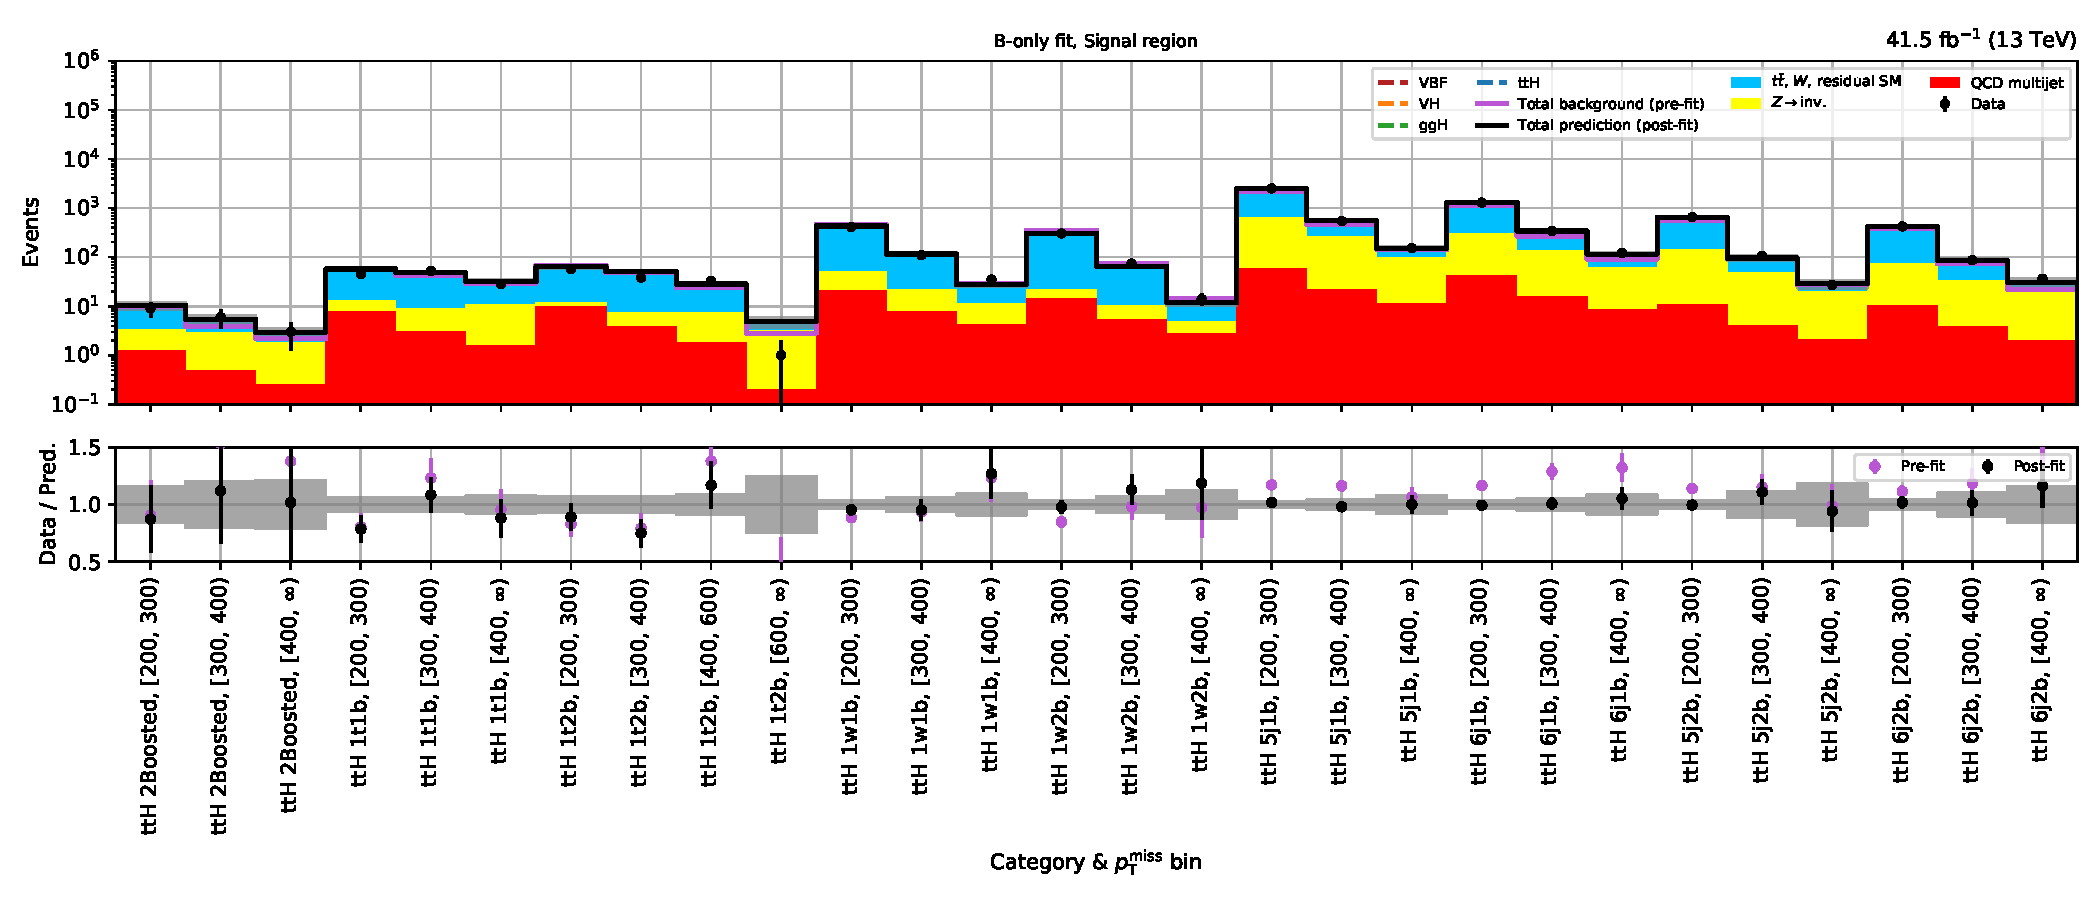
\includegraphics[width=\textwidth]{chapters/higgstoinv/figures/mountain_ranges/2017/ttH/SR_tree_fit_b-abs_values_ttH_cats.pdf}
        \caption{\ttH --- 2017}
    \end{subfigure}

    \begin{subfigure}[b]{0.9\textwidth}
        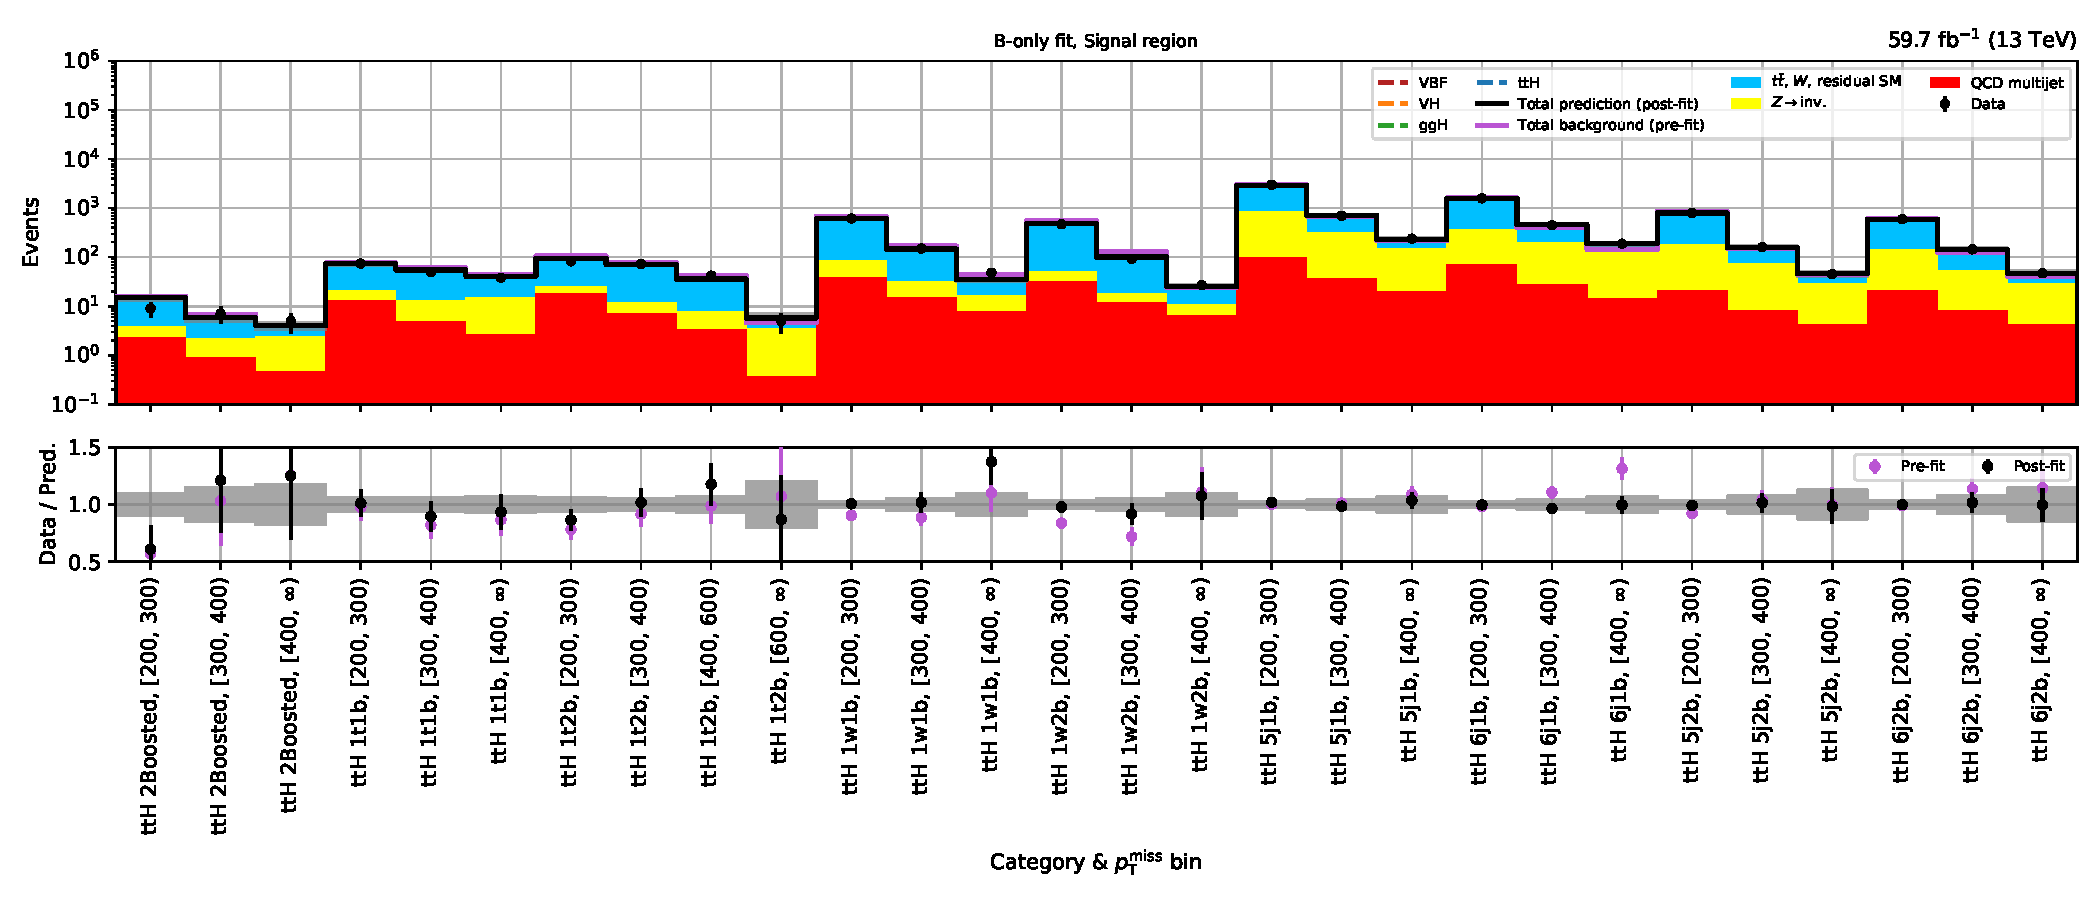
\includegraphics[width=\textwidth]{chapters/higgstoinv/figures/mountain_ranges/2018/ttH/SR_tree_fit_b-abs_values_ttH_cats.pdf}
        \caption{\ttH --- 2018}
    \end{subfigure}
    \caption[Results of the background-only fit to the \ttH categories in each year of Run-2]{Results of the background-only fit to the \ttH categories in each year of Run-2. ``Pre-fit'' refers to outcome of the control region-only prediction.}
    \label{fig:htoinv_mountain_range_B_only_ttH_SR}
\end{figure}

\clearpage


%=========================================================


\section{Background-only fits to the \texorpdfstring{\VH}{VH} categories}
\label{sec:B_only_fit_plots_VH_SR}

\begin{figure}[htbp]
    \centering
    \begin{subfigure}[b]{0.9\textwidth}
        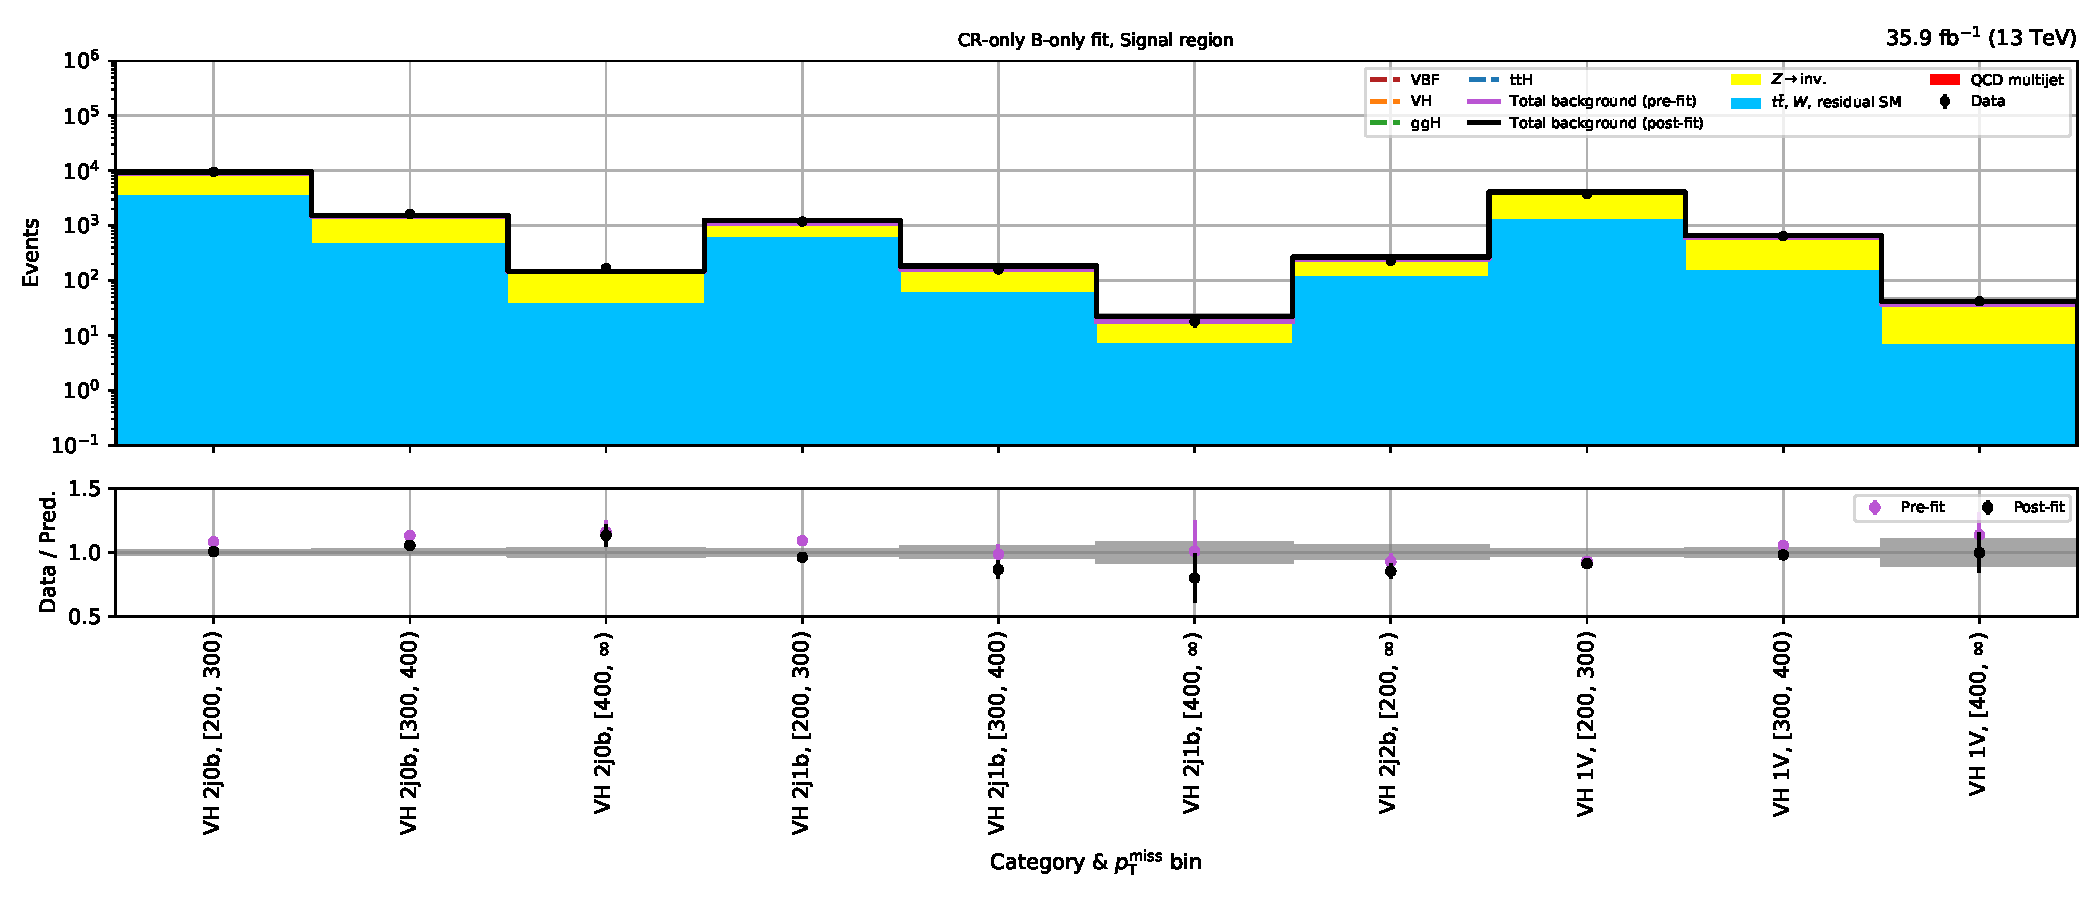
\includegraphics[width=\textwidth]{chapters/higgstoinv/figures/mountain_ranges/2016/VH/SR_tree_fit_b-abs_values_VH_cats.pdf}
        \caption{\VH --- 2016}
    \end{subfigure}

    \begin{subfigure}[b]{0.9\textwidth}
        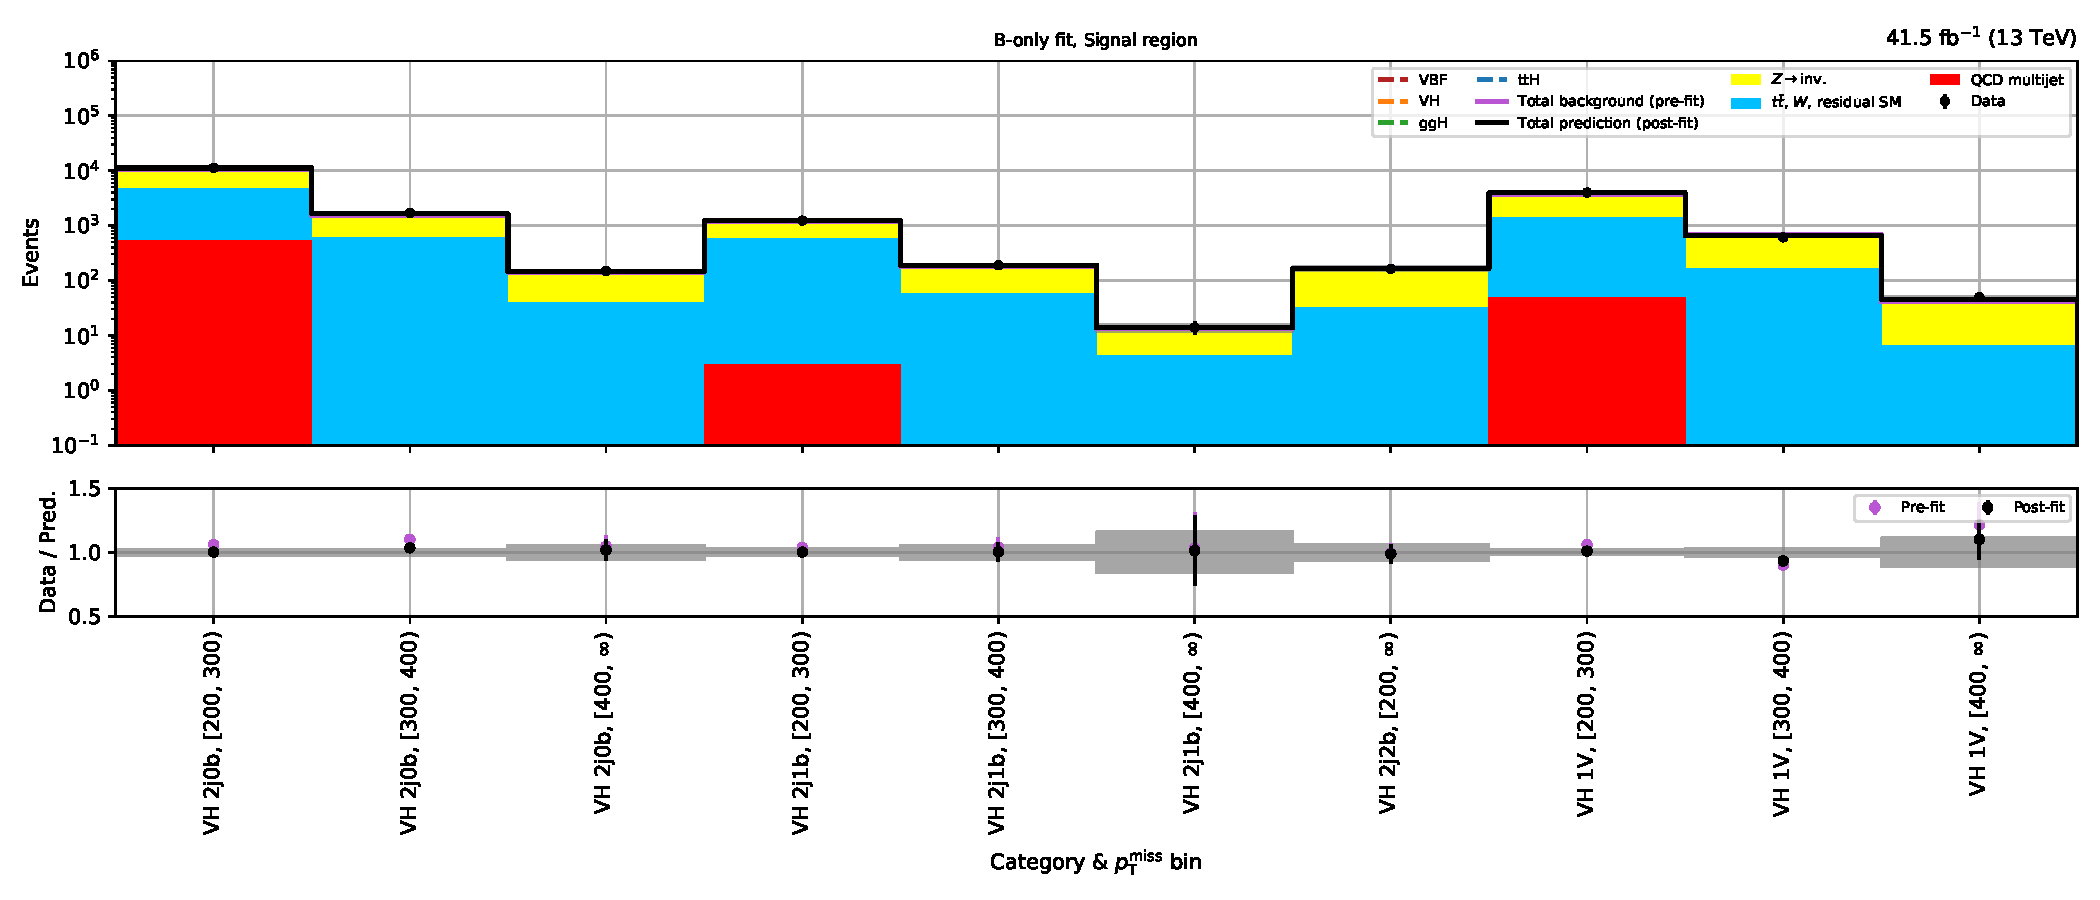
\includegraphics[width=\textwidth]{chapters/higgstoinv/figures/mountain_ranges/2017/VH/SR_tree_fit_b-abs_values_VH_cats.pdf}
        \caption{\VH --- 2017}
    \end{subfigure}

    \begin{subfigure}[b]{0.9\textwidth}
        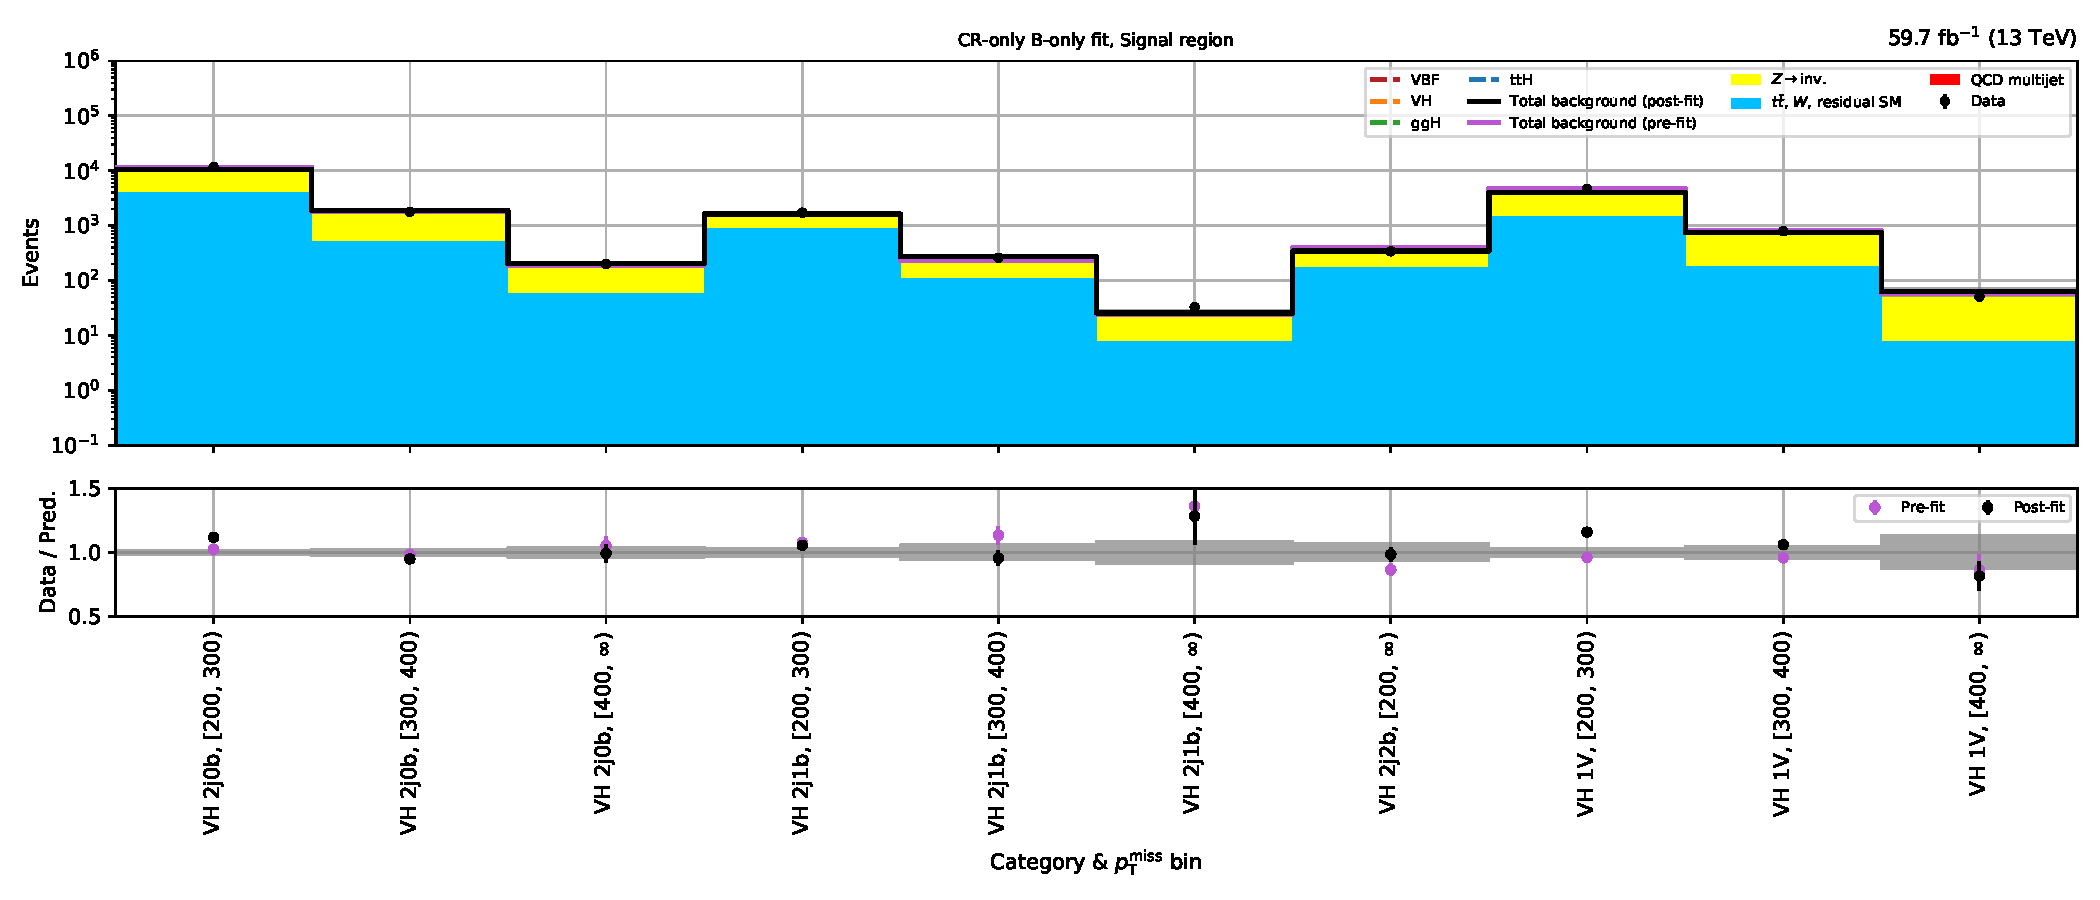
\includegraphics[width=\textwidth]{chapters/higgstoinv/figures/mountain_ranges/2018/VH/SR_tree_fit_b-abs_values_VH_cats.pdf}
        \caption{\VH --- 2018}
    \end{subfigure}
    \caption[Results of the background-only fit to the \VH categories in each year of Run-2]{Results of the background-only fit to the \VH categories in each year of Run-2. ``Pre-fit'' refers to outcome of the control region-only prediction.}
    \label{fig:htoinv_mountain_range_B_only_VH_SR}
\end{figure}

\clearpage


%=========================================================


\section{Signal region event counts after the background-only fit}
\label{sec:yield_tables_SR_B_only_fit}

% 2016:

\begin{table}[htbp]
    \footnotesize
    \centering
    \begin{tabular*}{\linewidth}{@{\extracolsep{\fill}}llccccr}
    \toprule
    Category & \ptmiss & Lost lepton & \ztonunu & QCD & Total SM & Data \\
    \midrule
    \ttH 2Boosted & [200, 300) &    $\text{7.88} \pm \text{1.04}$ &     $\text{0} \pm \text{0}$ &  $\text{0.88} \pm \text{0.27}$ &    $\text{8.76} \pm \text{1.08}$ &    12\\
        & [300, 400) &    $\text{3.03} \pm \text{0.52}$ &   $\text{0.84} \pm \text{0.54}$ &   $\text{0.32} \pm \text{0.1}$ &    $\text{4.19} \pm \text{0.75}$ &     1\\
        & [400, $\infty$) &    $\text{0.61} \pm \text{0.13}$ &    $\text{1.5} \pm \text{0.74}$ &  $\text{0.16} \pm \text{0.05}$ &    $\text{2.26} \pm \text{0.75}$ &     2\\
    \ttH 1t1b & [200, 300) &    $\text{32.6} \pm \text{2.52}$ &   $\text{5.79} \pm \text{1.64}$ &  $\text{5.97} \pm \text{1.82}$ &    $\text{44.3} \pm \text{3.51}$ &    36\\
        & [300, 400) &    $\text{27} \pm \text{2.39}$ &   $\text{7.15} \pm \text{1.56}$ &  $\text{2.24} \pm \text{0.67}$ &    $\text{36.4} \pm \text{2.93}$ &    45\\
        & [400, $\infty$) &    $\text{19.3} \pm \text{1.66}$ &    $\text{8.34} \pm \text{2.0}$ &  $\text{1.08} \pm \text{0.33}$ &    $\text{28.7} \pm \text{2.62}$ &    32\\
    \ttH 1t2b & [200, 300) &    $\text{44.2} \pm \text{2.72}$ &   $\text{3.02} \pm \text{1.28}$ &  $\text{7.95} \pm \text{2.44}$ &    $\text{55.2} \pm \text{3.88}$ &    51\\
        & [300, 400) &    $\text{40.3} \pm \text{2.58}$ &    $\text{2.38} \pm \text{1.1}$ &  $\text{2.94} \pm \text{0.87}$ &    $\text{45.6} \pm \text{2.94}$ &    40\\
        & [400, 600) &    $\text{17.1} \pm \text{1.61}$ &   $\text{4.49} \pm \text{1.62}$ &  $\text{1.28} \pm \text{0.39}$ &    $\text{22.8} \pm \text{2.32}$ &    21\\
        & [600, $\infty$) &    $\text{2.22} \pm \text{0.52}$ &   $\text{1.36} \pm \text{0.99}$ &  $\text{0.14} \pm \text{0.04}$ &    $\text{3.72} \pm \text{1.12}$ &     4\\
    \ttH 1W1b & [200, 300) &   $\text{362} \pm \text{11.7}$ &   $\text{41.3} \pm \text{8.72}$ &  $\text{18.1} \pm \text{5.54}$ &   $\text{422} \pm \text{15.6}$ &   396\\
        & [300, 400) &     $\text{81.5} \pm \text{5.1}$ &   $\text{32.4} \pm \text{7.12}$ &  $\text{6.71} \pm \text{2.04}$ &   $\text{121} \pm \text{8.99}$ &   112\\
        & [400, $\infty$) &    $\text{15.3} \pm \text{1.45}$ &   $\text{10.6} \pm \text{2.88}$ &  $\text{3.27} \pm \text{1.01}$ &    $\text{29.1} \pm \text{3.38}$ &    32\\
    \ttH 1W2b & [200, 300) &    $\text{260} \pm \text{9.2}$ &    $\text{3.9} \pm \text{2.19}$ &  $\text{12.2} \pm \text{3.77}$ &   $\text{276} \pm \text{10.2}$ &   264\\
        & [300, 400) &    $\text{51.3} \pm \text{3.26}$ &   $\text{4.41} \pm \text{2.52}$ &  $\text{4.53} \pm \text{1.38}$ &    $\text{60.3} \pm \text{4.35}$ &    65\\
        & [400, $\infty$) &     $\text{7.8} \pm \text{1.01}$ &    $\text{1.2} \pm \text{0.73}$ &  $\text{2.18} \pm \text{0.68}$ &    $\text{11.2} \pm \text{1.41}$ &    11\\
    \ttH 5j1b & [200, 300) &  $\text{1557} \pm \text{32.9}$ &  $\text{558} \pm \text{53.4}$ &  $\text{46.5} \pm \text{14.0}$ &  $\text{2161} \pm \text{64.3}$ &  2192\\
        & [300, 400) &   $\text{292} \pm \text{11.0}$ &  $\text{193} \pm \text{18.6}$ &  $\text{17.1} \pm \text{5.51}$ &   $\text{502} \pm \text{22.3}$ &   516\\
        & [400, $\infty$) &    $\text{54.5} \pm \text{4.13}$ &  $\text{119} \pm \text{12.6}$ &  $\text{8.25} \pm \text{2.51}$ &   $\text{182} \pm \text{13.5}$ &   189\\
    \ttH 6j1b & [200, 300) &   $\text{907} \pm \text{23.1}$ &  $\text{250} \pm \text{30.6}$ &  $\text{35.3} \pm \text{10.9}$ &  $\text{1192} \pm \text{39.9}$ &  1193\\
        & [300, 400) &    $\text{186} \pm \text{9.7}$ &  $\text{109} \pm \text{15.1}$ &  $\text{13} \pm \text{3.97}$ &   $\text{309} \pm \text{18.4}$ &   315\\
        & [400, $\infty$) &    $\text{51.5} \pm \text{3.68}$ &   $\text{50.1} \pm \text{10.1}$ &  $\text{6.31} \pm \text{1.92}$ &   $\text{108} \pm \text{10.9}$ &   114\\
    \ttH 5j2b & [200, 300) &   $\text{413} \pm \text{14.3}$ &  $\text{130} \pm \text{23.3}$ &  $\text{8.84} \pm \text{2.69}$ &   $\text{552} \pm \text{27.5}$ &   555\\
        & [300, 400) &    $\text{48.1} \pm \text{3.85}$ &   $\text{34.2} \pm \text{7.73}$ &  $\text{3.26} \pm \text{1.01}$ &     $\text{85.5} \pm \text{8.7}$ &    87\\
        & [400, $\infty$) &    $\text{9.32} \pm \text{1.42}$ &   $\text{22.6} \pm \text{4.15}$ &  $\text{1.57} \pm \text{0.48}$ &    $\text{33.4} \pm \text{4.41}$ &    36\\
    \ttH 6j2b & [200, 300) &   $\text{288} \pm \text{12.3}$ &   $\text{70.9} \pm \text{15.2}$ &   $\text{9.21} \pm \text{2.8}$ &   $\text{368} \pm \text{19.7}$ &   357\\
        & [300, 400) &    $\text{43.7} \pm \text{3.43}$ &   $\text{37.3} \pm \text{7.39}$ &  $\text{3.39} \pm \text{1.08}$ &    $\text{84.4} \pm \text{8.22}$ &    76\\
        & [400, $\infty$) &    $\text{12.8} \pm \text{1.94}$ &   $\text{11.3} \pm \text{4.77}$ &  $\text{1.65} \pm \text{0.51}$ &    $\text{25.7} \pm \text{5.17}$ &    29\\   
    \midrule
    \VH 2j0b & [200, 300) &  $\text{3804} \pm \text{72.6}$ &  $\text{5792} \pm \text{108}$ &  $\text{200} \pm \text{73.3}$ &  $\text{9796} \pm \text{150}$ &  9744\\
        & [300, 400) &   $\text{520} \pm \text{17.9}$ &   $\text{1090} \pm \text{24.8}$ &     $\text{0} \pm \text{0}$ &   $\text{1610} \pm \text{30.6}$ &  1663\\
        & [400, $\infty$) &    $\text{51.5} \pm \text{5.63}$ &    $\text{109} \pm \text{7.55}$ &     $\text{0} \pm \text{0}$ &    $\text{161} \pm \text{9.42}$ &   172\\
    \VH 2j1b & [200, 300) &   $\text{535} \pm \text{18.2}$ &    $\text{520} \pm \text{21.4}$ &    $\text{1.1} \pm \text{0.41}$ &   $\text{1056} \pm \text{28.1}$ &  1060\\
        & [300, 400) &    $\text{52.5} \pm \text{4.32}$ &    $\text{101} \pm \text{7.62}$ &     $\text{0} \pm \text{0}$ &    $\text{153} \pm \text{8.76}$ &   139\\
        & [400, $\infty$) &     $\text{3.35} \pm \text{1.0}$ &     $\text{10.4} \pm \text{2.15}$ &     $\text{0} \pm \text{0}$ &     $\text{13.7} \pm \text{2.37}$ &    14\\
    \VH 2j2b & [200, $\infty$) &    $\text{35.4} \pm \text{3.84}$ &    $\text{125} \pm \text{10.4}$ &     $\text{0} \pm \text{0}$ &    $\text{160} \pm \text{11.1}$ &   143\\
    \VH 1V & [200, 300) &  $\text{1459} \pm \text{37.1}$ &   $\text{2521} \pm \text{55.8}$ &   $\text{18.3} \pm \text{6.71}$ &   $\text{3998} \pm \text{67.4}$ &  3899\\
        & [300, 400) &   $\text{162} \pm \text{9.69}$ &    $\text{484} \pm \text{17.8}$ &     $\text{0} \pm \text{0}$ &    $\text{646} \pm \text{20.2}$ &   654\\
        & [400, $\infty$) &    $\text{7.51} \pm \text{1.41}$ &     $\text{28} \pm \text{4.17}$ &     $\text{0} \pm \text{0}$ &      $\text{35.5} \pm \text{4.4}$ &    42\\
    \bottomrule
    \end{tabular*}
    \caption[Event counts in the signal region after the background-only fit to data in 2016]{Event counts in the signal region after the background-only fit to data in 2016.}
    \label{tab:yields_SR_B_only_2016}
\end{table}

% 2017:

\begin{table}[htbp]
    \small
    \centering
    \begin{tabular*}{\linewidth}{@{\extracolsep{\fill}}llccccr}
    \toprule
    Category & \ptmiss & Lost lepton & \ztonunu & QCD & Total SM & Data \\
    \midrule
    \ttH 2Boosted & [200, 300) &    $\text{7.03} \pm \text{0.95}$ &   $\text{2.04} \pm \text{1.04}$ &  $\text{1.28} \pm \text{0.35}$ &    $\text{10.4} \pm \text{1.45}$ &     9 \\
        & [300, 400) &    $\text{2.49} \pm \text{0.32}$ &   $\text{2.39} \pm \text{1.01}$ &  $\text{0.49} \pm \text{0.13}$ &    $\text{5.37} \pm \text{1.07}$ &     6 \\
        & [400, $\infty$) &    $\text{1.13} \pm \text{0.24}$ &   $\text{1.56} \pm \text{0.54}$ &  $\text{0.25} \pm \text{0.07}$ &    $\text{2.95} \pm \text{0.59}$ &     3 \\
    \ttH 1t1b & [200, 300) &    $\text{44.4} \pm \text{2.64}$ &   $\text{4.95} \pm \text{1.29}$ &  $\text{8.05} \pm \text{2.26}$ &    $\text{57.4} \pm \text{3.71}$ &    45 \\
        & [300, 400) &    $\text{38.8} \pm \text{2.79}$ &    $\text{6.07} \pm \text{1.1}$ &  $\text{3.12} \pm \text{0.88}$ &    $\text{48.0} \pm \text{3.12}$ &    52 \\
        & [400, $\infty$) &    $\text{20.8} \pm \text{1.63}$ &   $\text{9.34} \pm \text{1.72}$ &  $\text{1.62} \pm \text{0.45}$ &    $\text{31.8} \pm \text{2.41}$ &    28 \\
    \ttH 1t2b & [200, 300) &    $\text{51.9} \pm \text{3.12}$ &    $\text{2.1} \pm \text{1.11}$ &  $\text{10.1} \pm \text{2.74}$ &    $\text{64.2} \pm \text{4.29}$ &    57 \\
        & [300, 400) &    $\text{43.2} \pm \text{2.72}$ &   $\text{3.72} \pm \text{1.24}$ &  $\text{3.86} \pm \text{1.05}$ &    $\text{50.7} \pm \text{3.17}$ &    38 \\
        & [400, 600) &     $\text{20.9} \pm \text{2.0}$ &   $\text{5.53} \pm \text{1.79}$ &  $\text{1.83} \pm \text{0.51}$ &    $\text{28.3} \pm \text{2.73}$ &    33 \\
        & [600, $\infty$) &    $\text{1.57} \pm \text{0.37}$ &   $\text{3.01} \pm \text{1.06}$ &   $\text{0.2} \pm \text{0.06}$ &    $\text{4.79} \pm \text{1.12}$ &     1 \\
    \ttH 1W1b & [200, 300) &   $\text{378} \pm \text{12.6}$ &   $\text{30.1} \pm \text{5.82}$ &  $\text{21.3} \pm \text{5.83}$ &   $\text{430} \pm \text{15.0}$ &   410 \\
        & [300, 400) &    $\text{93.8} \pm \text{4.48}$ &   $\text{13.8} \pm \text{4.38}$ &  $\text{8.14} \pm \text{2.25}$ &   $\text{116} \pm \text{6.66}$ &   110 \\
        & [400, $\infty$) &    $\text{16.4} \pm \text{1.35}$ &   $\text{6.95} \pm \text{1.78}$ &   $\text{4.3} \pm \text{1.19}$ &    $\text{27.6} \pm \text{2.53}$ &    35 \\
    \ttH 1W2b & [200, 300) &   $\text{286} \pm \text{11.5}$ &    $\text{7.8} \pm \text{3.38}$ &  $\text{14.5} \pm \text{3.93}$ &   $\text{309} \pm \text{12.6}$ &   302 \\
        & [300, 400) &    $\text{54.9} \pm \text{3.56}$ &   $\text{5.11} \pm \text{2.46}$ &  $\text{5.56} \pm \text{1.57}$ &     $\text{65.6} \pm \text{4.6}$ &    74 \\
        & [400, $\infty$) &    $\text{6.92} \pm \text{0.88}$ &   $\text{2.04} \pm \text{0.71}$ &  $\text{2.88} \pm \text{0.79}$ &    $\text{11.8} \pm \text{1.39}$ &    14 \\
    \ttH 5j1b & [200, 300) &  $\text{1842} \pm \text{33.1}$ &  $\text{570} \pm \text{48.7}$ &  $\text{59.1} \pm \text{16.5}$ &  $\text{2471} \pm \text{61.2}$ &  2514 \\
        & [300, 400) &   $\text{290} \pm \text{10.4}$ &  $\text{239} \pm \text{21.9}$ &  $\text{22.1} \pm \text{6.49}$ &   $\text{551} \pm \text{25.1}$ &   540 \\
        & [400, $\infty$) &    $\text{54.6} \pm \text{3.61}$ &   $\text{85.6} \pm \text{11.9}$ &  $\text{11.6} \pm \text{3.24}$ &   $\text{152} \pm \text{12.9}$ &   152 \\
    \ttH 6j1b & [200, 300) &  $\text{1001} \pm \text{22.2}$ &  $\text{259} \pm \text{32.5}$ &  $\text{43.2} \pm \text{12.2}$ &  $\text{1303} \pm \text{41.2}$ &  1295 \\
        & [300, 400) &   $\text{204} \pm \text{8.13}$ &  $\text{120} \pm \text{15.5}$ &  $\text{16.5} \pm \text{4.66}$ &   $\text{341} \pm \text{18.1}$ &   343 \\
        & [400, $\infty$) &    $\text{54.3} \pm \text{3.89}$ &   $\text{52.2} \pm \text{9.05}$ &  $\text{8.59} \pm \text{2.48}$ &   $\text{115} \pm \text{10.2}$ &   121 \\
    \ttH 5j2b & [200, 300) &   $\text{515} \pm \text{15.4}$ &  $\text{129} \pm \text{19.0}$ &  $\text{10.9} \pm \text{2.93}$ &   $\text{654} \pm \text{24.6}$ &   651 \\
        & [300, 400) &    $\text{47.5} \pm \text{3.67}$ &   $\text{44.0} \pm \text{8.57}$ &  $\text{4.14} \pm \text{1.16}$ &    $\text{95.7} \pm \text{9.39}$ &   106 \\
        & [400, $\infty$) &     $\text{8.59} \pm \text{1.2}$ &   $\text{17.9} \pm \text{4.75}$ &  $\text{2.14} \pm \text{0.58}$ &    $\text{28.7} \pm \text{4.93}$ &    27 \\
    \ttH 6j2b & [200, 300) &   $\text{340} \pm \text{11.5}$ &   $\text{64.9} \pm \text{14.6}$ &  $\text{10.4} \pm \text{2.87}$ &   $\text{415} \pm \text{18.8}$ &   422 \\
        & [300, 400) &    $\text{51.8} \pm \text{4.39}$ &   $\text{30.0} \pm \text{7.21}$ &  $\text{3.94} \pm \text{1.12}$ &    $\text{85.8} \pm \text{8.51}$ &    87 \\
        & [400, $\infty$) &    $\text{7.05} \pm \text{1.14}$ &   $\text{21.8} \pm \text{4.79}$ &  $\text{2.05} \pm \text{0.56}$ &    $\text{30.9} \pm \text{4.96}$ &    36 \\
        \midrule
    \VH 2j0b & [200, 300) &  $\text{4225} \pm \text{76.3}$ &  $\text{6459} \pm \text{162}$ &  $\text{546} \pm \text{194}$ &  $\text{11230} \pm \text{264}$ &  11263 \\
        & [300, 400) &   $\text{605} \pm \text{23.5}$ &   $\text{1033} \pm \text{26.3}$ &      $\text{0} \pm \text{0}$ &    $\text{1638} \pm \text{35.3}$ &   1696 \\
        & [400, $\infty$) &     $\text{40} \pm \text{3.7}$ &    $\text{106} \pm \text{7.53}$ &      $\text{0} \pm \text{0}$ &     $\text{146} \pm \text{8.39}$ &    149 \\
    \VH 2j1b & [200, 300) &   $\text{577} \pm \text{18.2}$ &    $\text{652} \pm \text{26.8}$ &     $\text{2.94} \pm \text{1.1}$ &    $\text{1232} \pm \text{32.4}$ &   1235 \\
        & [300, 400) &     $\text{57.4} \pm \text{4.8}$ &    $\text{132} \pm \text{9.66}$ &      $\text{0} \pm \text{0}$ &     $\text{189} \pm \text{10.8}$ &    190 \\
        & [400, $\infty$) &    $\text{4.27} \pm \text{1.06}$ &     $\text{9.54} \pm \text{1.93}$ &      $\text{0} \pm \text{0}$ &       $\text{13.8} \pm \text{2.2}$ &     14 \\
    \VH 2j2b & [200, $\infty$) &    $\text{32.9} \pm \text{3.48}$ &    $\text{133} \pm \text{10.2}$ &      $\text{0} \pm \text{0}$ &     $\text{166} \pm \text{10.8}$ &    164 \\       
    \VH 1V & [200, 300) &  $\text{1381} \pm \text{39.3}$ &   $\text{2536} \pm \text{65.7}$ &    $\text{49.2} \pm \text{18.7}$ &    $\text{3965} \pm \text{78.8}$ &   4005 \\
        & [300, 400) &   $\text{167} \pm \text{8.61}$ &    $\text{489} \pm \text{19.7}$ &      $\text{0} \pm \text{0}$ &     $\text{656} \pm \text{21.5}$ &    612 \\
        & [400, $\infty$) &    $\text{6.53} \pm \text{0.95}$ &      $\text{38.9} \pm \text{5.0}$ &      $\text{0} \pm \text{0}$ &      $\text{45.4} \pm \text{5.09}$ &     50 \\
       \bottomrule
    \end{tabular*}
    \caption[Event counts in the signal region after the background-only fit to data in 2017]{Event counts in the signal region after the background-only fit to data in 2017.}
    \label{tab:yields_SR_B_only_2017}
\end{table}

% 2018:

\begin{table}[htbp]
    \small
    \centering
    \begin{tabular*}{\linewidth}{@{\extracolsep{\fill}}llccccr}
    \toprule
    Category & \ptmiss & Lost lepton & \ztonunu & QCD & Total SM & Data \\
    \midrule
    \ttH 2Boosted & [200, 300) &    $\text{11.0} \pm \text{1.05}$ &   $\text{1.52} \pm \text{0.89}$ &  $\text{2.25} \pm \text{0.51}$ &    $\text{14.8} \pm \text{1.47}$ &     9 \\
        & [300, 400) &    $\text{3.54} \pm \text{0.45}$ &   $\text{1.35} \pm \text{0.73}$ &   $\text{0.88} \pm \text{0.2}$ &    $\text{5.78} \pm \text{0.88}$ &     7 \\
        & [400, $\infty$) &    $\text{1.64} \pm \text{0.34}$ &    $\text{1.9} \pm \text{0.61}$ &   $\text{0.46} \pm \text{0.1}$ &      $\text{4.0} \pm \text{0.7}$ &     5 \\
    \ttH 1t1b & [200, 300) &    $\text{52.7} \pm \text{2.93}$ &   $\text{7.68} \pm \text{1.29}$ &  $\text{12.8} \pm \text{2.89}$ &    $\text{73.2} \pm \text{4.31}$ &    74 \\
        & [300, 400) &    $\text{41.5} \pm \text{2.76}$ &   $\text{8.29} \pm \text{1.11}$ &  $\text{4.95} \pm \text{1.06}$ &    $\text{54.7} \pm \text{3.16}$ &    49 \\
        & [400, $\infty$) &    $\text{25.6} \pm \text{1.81}$ &   $\text{12.5} \pm \text{2.22}$ &  $\text{2.59} \pm \text{0.58}$ &    $\text{40.7} \pm \text{2.93}$ &    38 \\
    \ttH 1t2b & [200, 300) &    $\text{70.2} \pm \text{3.63}$ &   $\text{6.67} \pm \text{1.76}$ &  $\text{18.0} \pm \text{3.85}$ &    $\text{94.8} \pm \text{5.57}$ &    82 \\
        & [300, 400) &    $\text{58.9} \pm \text{3.39}$ &   $\text{4.69} \pm \text{1.31}$ &  $\text{7.17} \pm \text{1.61}$ &    $\text{70.8} \pm \text{3.98}$ &    72 \\
        & [400, 600) &    $\text{28.0} \pm \text{1.98}$ &   $\text{4.26} \pm \text{1.47}$ &  $\text{3.38} \pm \text{0.77}$ &    $\text{35.7} \pm \text{2.58}$ &    42 \\
        & [600, $\infty$) &    $\text{2.24} \pm \text{0.44}$ &   $\text{3.15} \pm \text{1.08}$ &  $\text{0.37} \pm \text{0.08}$ &    $\text{5.76} \pm \text{1.16}$ &     5 \\
    \ttH 1W1b & [200, 300) &   $\text{522} \pm \text{12.8}$ &   $\text{48.5} \pm \text{8.15}$ &   $\text{37.9} \pm \text{8.5}$ &   $\text{608} \pm \text{17.4}$ &   612 \\
        & [300, 400) &   $\text{115} \pm \text{5.28}$ &   $\text{17.0} \pm \text{4.18}$ &  $\text{14.7} \pm \text{3.38}$ &   $\text{146} \pm \text{7.53}$ &   149 \\
        & [400, $\infty$) &    $\text{18.4} \pm \text{1.46}$ &   $\text{8.65} \pm \text{2.47}$ &  $\text{7.89} \pm \text{1.87}$ &    $\text{35.0} \pm \text{3.43}$ &    48 \\
    \ttH 1W2b & [200, 300) &   $\text{426} \pm \text{12.3}$ &   $\text{20.3} \pm \text{5.64}$ &  $\text{31.2} \pm \text{6.93}$ &   $\text{478} \pm \text{15.2}$ &   467 \\
        & [300, 400) &    $\text{82.6} \pm \text{3.82}$ &   $\text{5.71} \pm \text{2.46}$ &  $\text{12.1} \pm \text{2.84}$ &   $\text{100} \pm \text{5.36}$ &    92 \\
        & [400, $\infty$) &    $\text{14.2} \pm \text{1.25}$ &    $\text{4.5} \pm \text{1.47}$ &   $\text{6.4} \pm \text{1.45}$ &    $\text{25.1} \pm \text{2.42}$ &    27 \\
    \ttH 5j1b & [200, 300) &  $\text{2074} \pm \text{33.6}$ &  $\text{761} \pm \text{56.3}$ &  $\text{97.6} \pm \text{22.1}$ &  $\text{2933} \pm \text{69.2}$ &  2989 \\
        & [300, 400) &   $\text{387} \pm \text{13.5}$ &  $\text{284} \pm \text{23.7}$ &  $\text{37.0} \pm \text{8.75}$ &   $\text{708} \pm \text{28.7}$ &   698 \\
        & [400, $\infty$) &    $\text{80.8} \pm \text{4.84}$ &  $\text{129} \pm \text{14.2}$ &  $\text{19.6} \pm \text{4.65}$ &   $\text{230} \pm \text{15.7}$ &   238 \\
    \ttH 6j1b & [200, 300) &  $\text{1207} \pm \text{25.2}$ &  $\text{302} \pm \text{29.1}$ &  $\text{70.1} \pm \text{16.2}$ &  $\text{1579} \pm \text{41.7}$ &  1574 \\
        & [300, 400) &   $\text{258} \pm \text{9.96}$ &  $\text{176} \pm \text{17.6}$ &  $\text{27.1} \pm \text{6.29}$ &   $\text{461} \pm \text{21.2}$ &   445 \\
        & [400, $\infty$) &    $\text{63.2} \pm \text{3.97}$ &  $\text{111} \pm \text{12.9}$ &  $\text{14.2} \pm \text{3.32}$ &   $\text{189} \pm \text{13.9}$ &   188 \\
    \ttH 5j2b & [200, 300) &   $\text{612} \pm \text{15.7}$ &  $\text{161} \pm \text{21.9}$ &  $\text{21.1} \pm \text{4.97}$ &   $\text{794} \pm \text{27.4}$ &   788 \\
        & [300, 400) &    $\text{82.8} \pm \text{5.01}$ &   $\text{65.7} \pm \text{10.4}$ &  $\text{8.24} \pm \text{1.82}$ &   $\text{157} \pm \text{11.7}$ &   159 \\
        & [400, $\infty$) &    $\text{16.5} \pm \text{1.62}$ &    $\text{25} \pm \text{5.5}$ &  $\text{4.29} \pm \text{0.98}$ &    $\text{45.8} \pm \text{5.81}$ &    45 \\
    \ttH 6j2b & [200, 300) &   $\text{450} \pm \text{13.6}$ &  $\text{123} \pm \text{18.0}$ &  $\text{21.2} \pm \text{4.79}$ &   $\text{594} \pm \text{23.1}$ &   593 \\
        & [300, 400) &    $\text{87.1} \pm \text{5.78}$ &    $\text{46.3} \pm \text{9.9}$ &  $\text{8.27} \pm \text{1.85}$ &   $\text{142} \pm \text{11.6}$ &   144 \\
        & [400, $\infty$) &    $\text{18.8} \pm \text{2.28}$ &   $\text{24.1} \pm \text{6.38}$ &   $\text{4.31} \pm \text{1.0}$ &    $\text{47.1} \pm \text{6.85}$ &    47 \\
    \midrule
    \VH 2j0b & [200, 300) &  $\text{4560} \pm \text{65.9}$ &  $\text{7298} \pm \text{132}$ &  $\text{321} \pm \text{112}$ &  $\text{12180} \pm \text{185}$ &  12086 \\
        & [300, 400) &   $\text{561} \pm \text{19.5}$ &   $\text{1231} \pm \text{25.9}$ &      $\text{0} \pm \text{0}$ &    $\text{1792} \pm \text{32.4}$ &   1827 \\
        & [400, $\infty$) &    $\text{67.7} \pm \text{7.05}$ &     $\text{135} \pm \text{8.7}$ &      $\text{0} \pm \text{0}$ &     $\text{202} \pm \text{11.2}$ &    208 \\
    \VH 2j1b & [200, 300) &   $\text{729} \pm \text{19.9}$ &    $\text{747} \pm \text{31.1}$ &     $\text{1.8} \pm \text{0.64}$ &    $\text{1477} \pm \text{36.9}$ &   1519 \\
        & [300, 400) &    $\text{95.7} \pm \text{5.76}$ &    $\text{140} \pm \text{9.24}$ &      $\text{0} \pm \text{0}$ &     $\text{235} \pm \text{10.9}$ &    236 \\
        & [400, $\infty$) &    $\text{7.81} \pm \text{1.69}$ &     $\text{18.7} \pm \text{2.95}$ &      $\text{0} \pm \text{0}$ &       $\text{26.5} \pm \text{3.4}$ &     27 \\
    \VH 2j2b & [200, $\infty$) &    $\text{56.3} \pm \text{4.52}$ &    $\text{182} \pm \text{13.1}$ &      $\text{0} \pm \text{0}$ &     $\text{238} \pm \text{13.8}$ &    208 \\
    \VH 1V & [200, 300) &  $\text{1545} \pm \text{34.7}$ &   $\text{3049} \pm \text{63.1}$ &    $\text{30.4} \pm \text{11.0}$ &    $\text{4625} \pm \text{72.9}$ &   4815 \\
        & [300, 400) &    $\text{179} \pm \text{7.8}$ &    $\text{617} \pm \text{20.1}$ &      $\text{0} \pm \text{0}$ &     $\text{796} \pm \text{21.6}$ &    816 \\
        & [400, $\infty$) &    $\text{5.95} \pm \text{0.85}$ &     $\text{58.9} \pm \text{5.64}$ &      $\text{0} \pm \text{0}$ &       $\text{64.9} \pm \text{5.7}$ &     51 \\
    \bottomrule
\end{tabular*}
\caption[Event counts in the signal region after the background-only fit to data in 2018]{Event counts in the signal region after the background-only fit to data in 2018.}
\label{tab:yields_SR_B_only_2018}
\end{table}

\clearpage


%=========================================================


\section{Limits and likelihood scans for each category}
\label{sec:limits_likelihoods_cats_supplementary}

\begin{figure}[htbp]
    \centering
    \begin{subfigure}[b]{0.45\textwidth}
        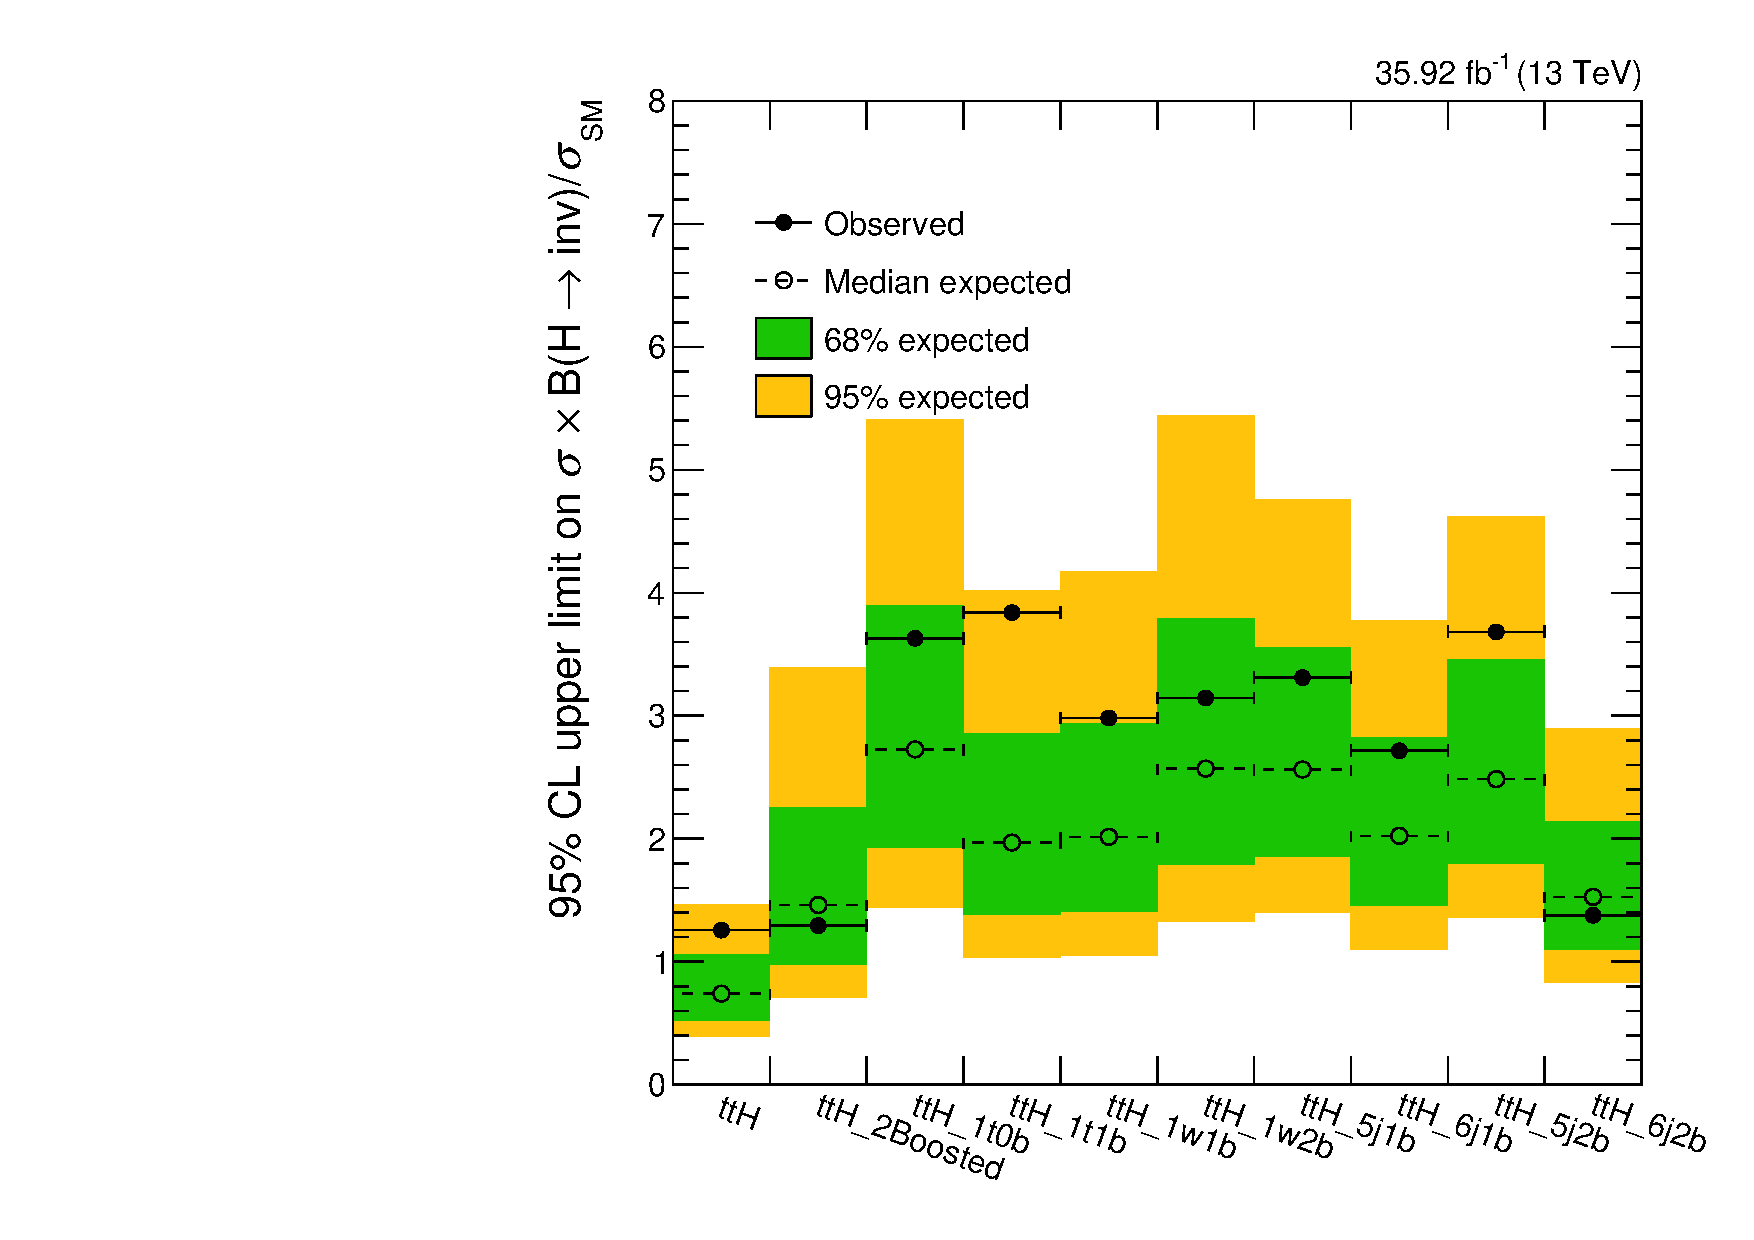
\includegraphics[width=\textwidth]{chapters/higgstoinv/figures/limits/ttH/limit_2016_ttH.pdf}
        \caption{\ttH --- 2016}
    \end{subfigure}
    \hfill
    \begin{subfigure}[b]{0.45\textwidth}
        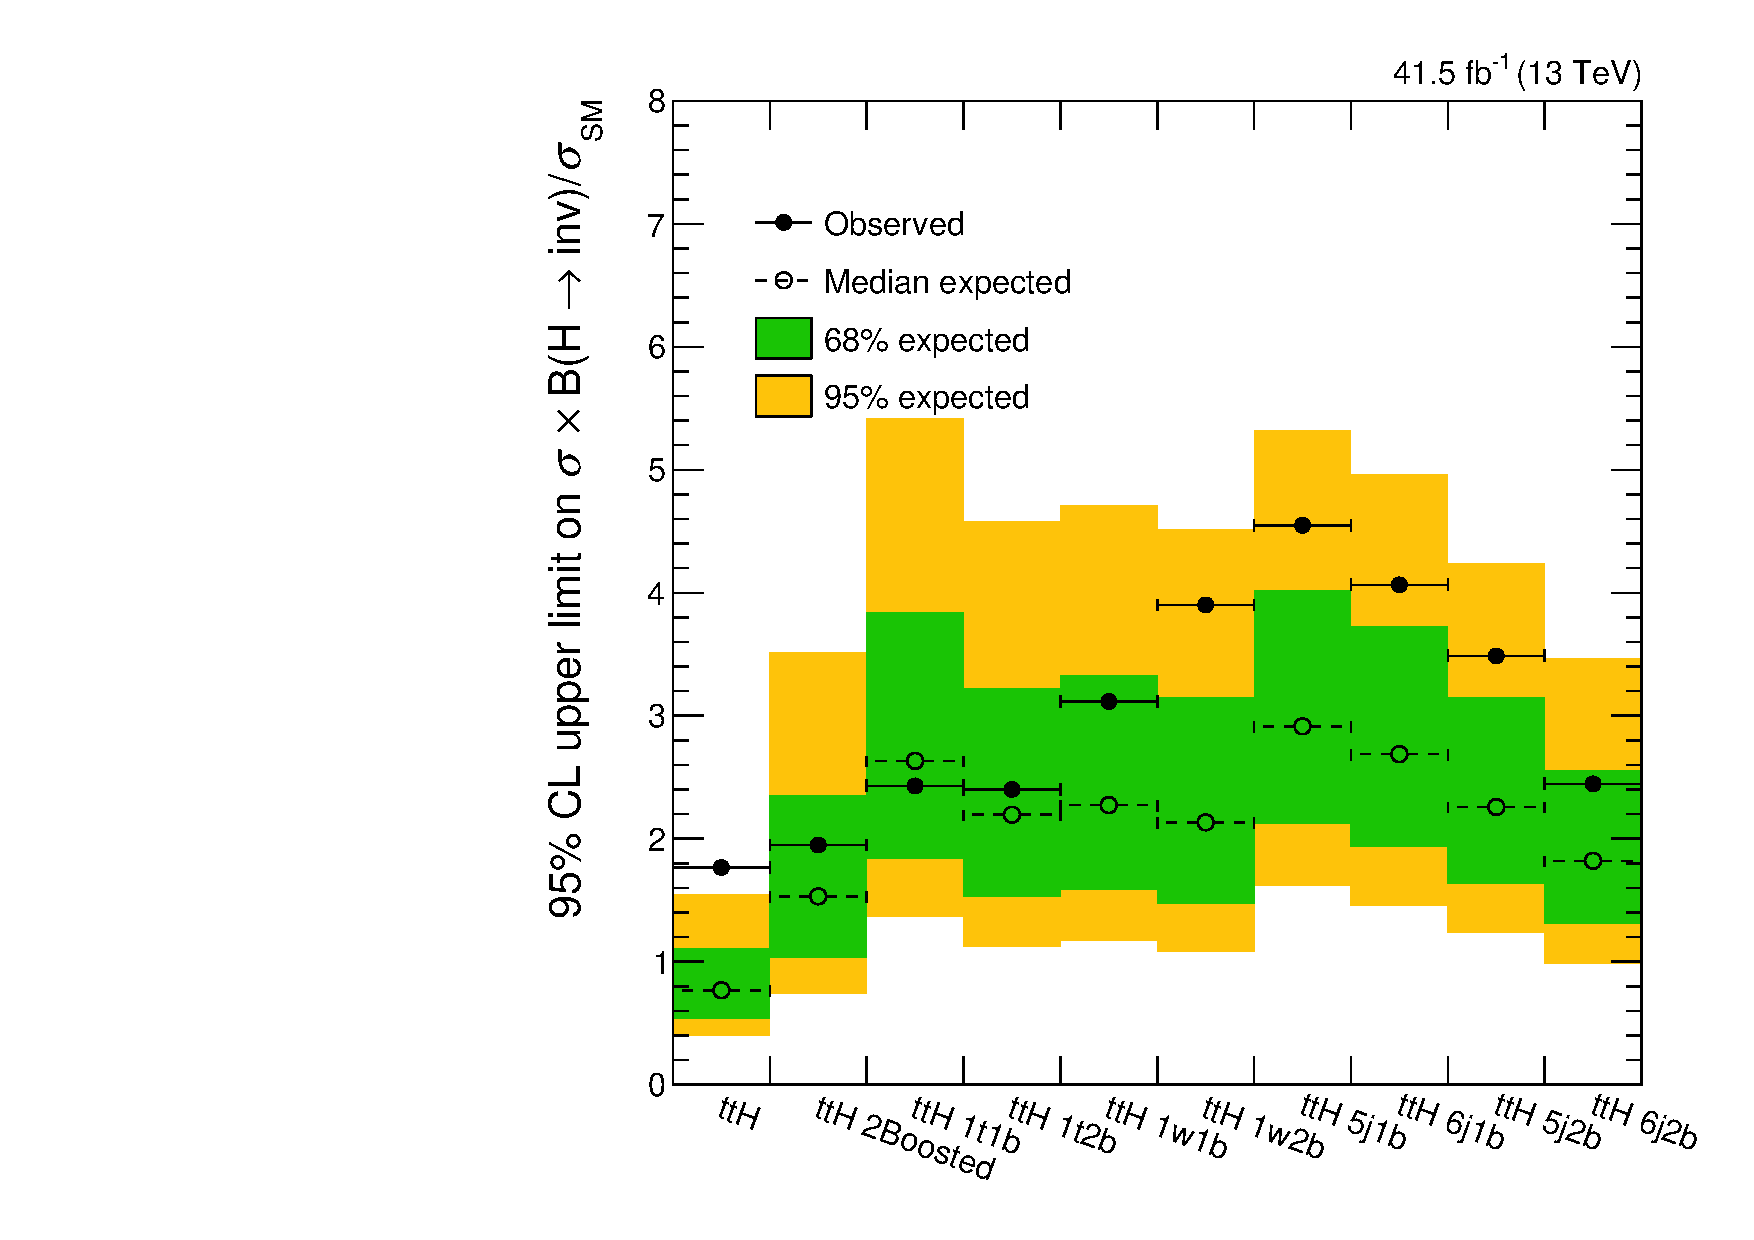
\includegraphics[width=\textwidth]{chapters/higgstoinv/figures/limits/ttH/limit_2017_ttH.pdf}
        \caption{\ttH --- 2017}
    \end{subfigure}

    \begin{subfigure}[b]{0.45\textwidth}
        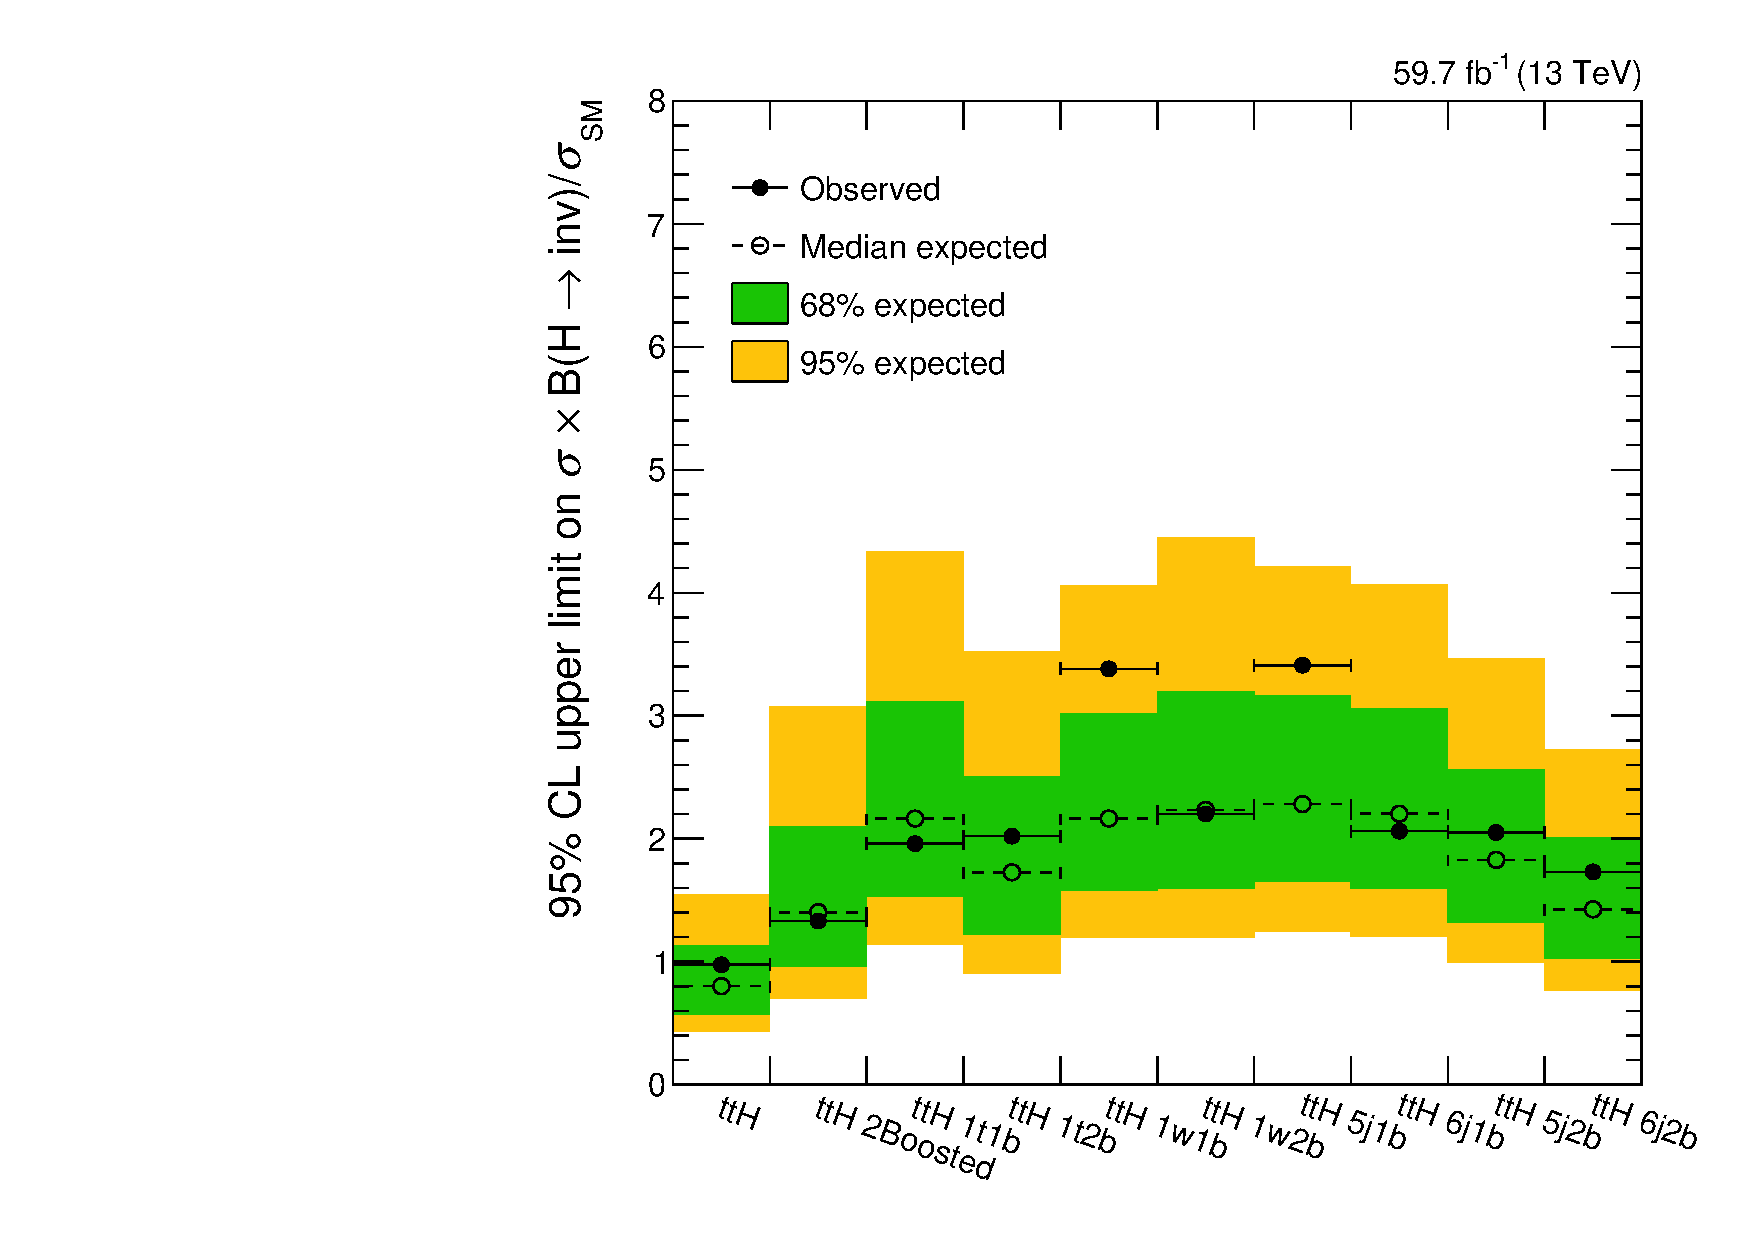
\includegraphics[width=\textwidth]{chapters/higgstoinv/figures/limits/ttH/limit_2018_ttH.pdf}
        \caption{\ttH --- 2018}
    \end{subfigure}
    \caption[Observed and expected 95\,\% CL upper limits on the Higgs boson to invisible state branching fraction in the \ttH channel, for both the individual categories, and the combination of them, for each data-taking year in Run-2]{Observed and expected 95\,\% CL upper limits on the Higgs boson to invisible state branching fraction in the \ttH channel, for both the individual categories, and the combination of them, for each data-taking year in Run-2.}
    \label{fig:htoinv_limit_ttH_per_year}
\end{figure}

\begin{figure}[htbp]
    \centering
    \begin{subfigure}[b]{0.45\textwidth}
        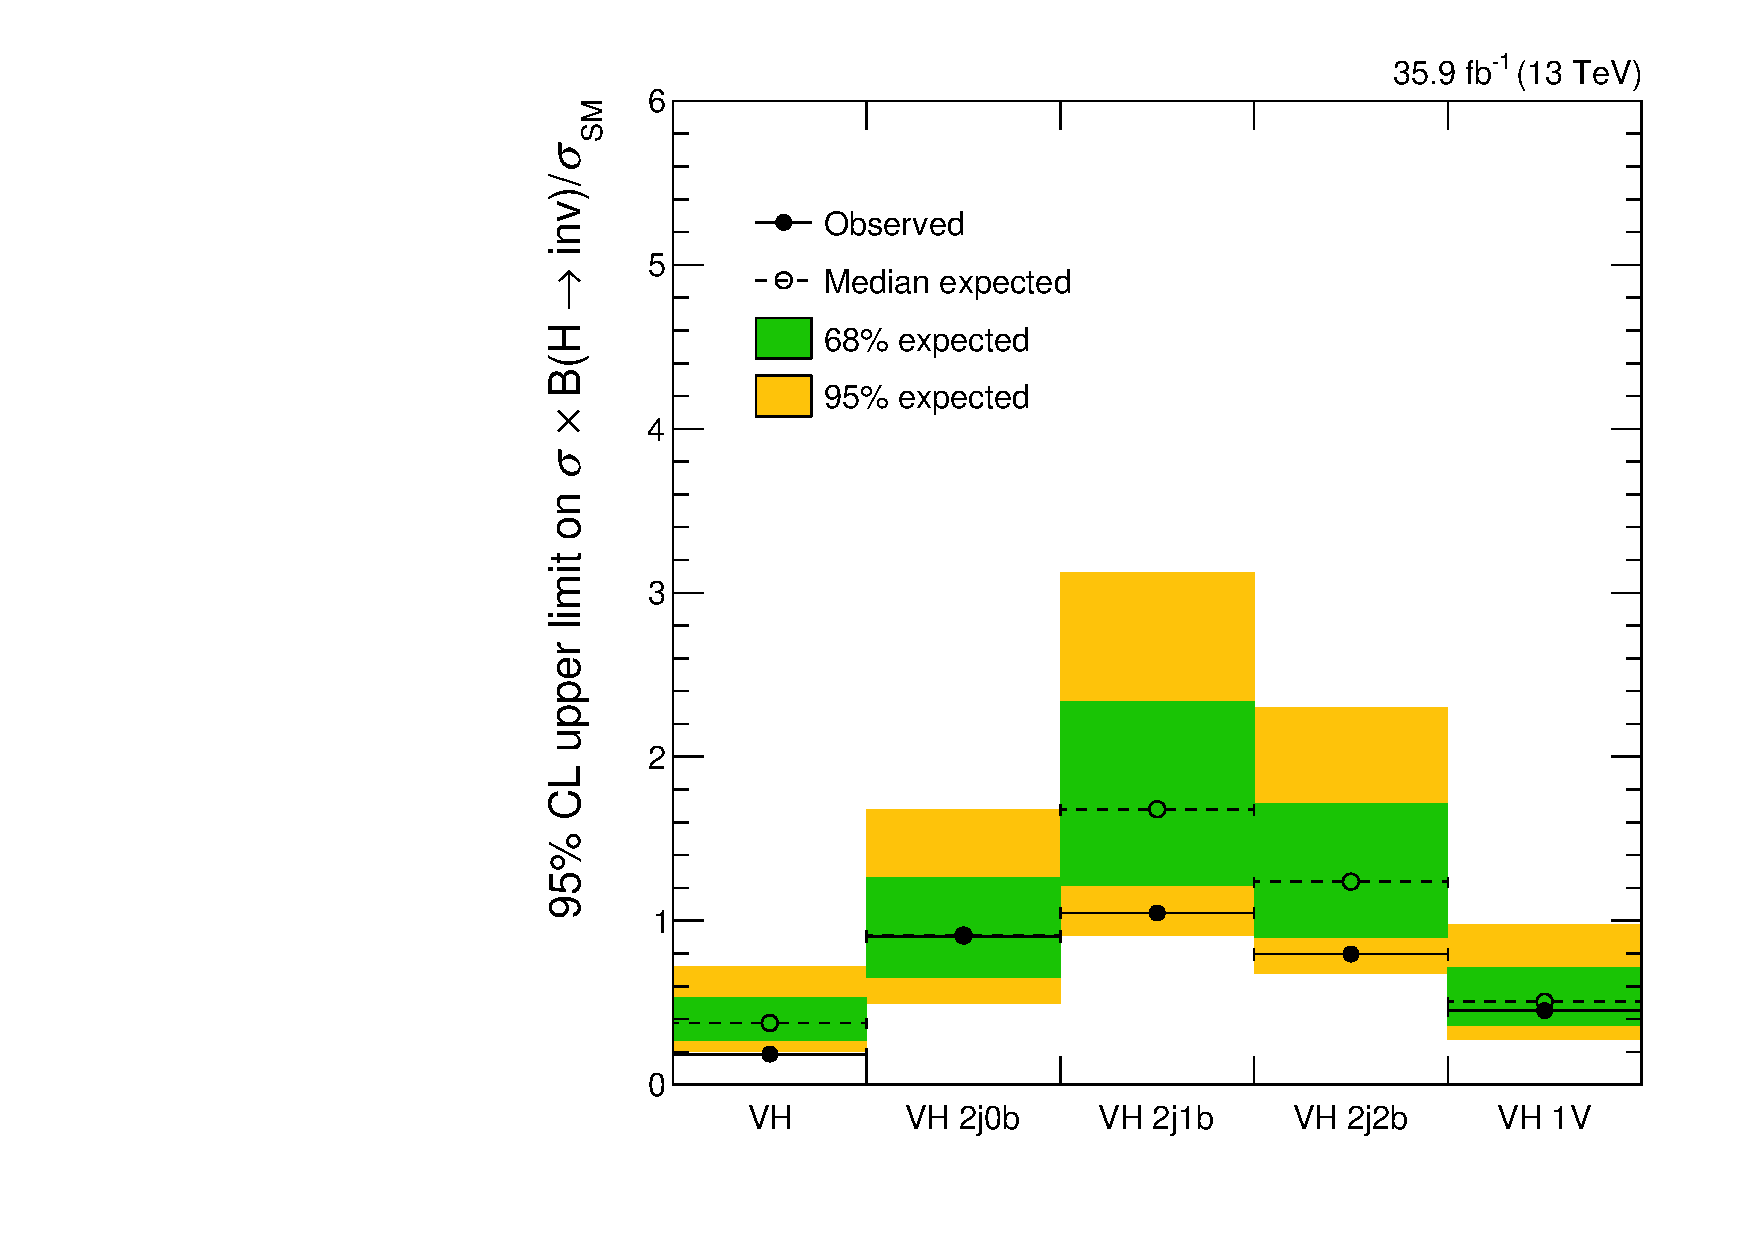
\includegraphics[width=\textwidth]{chapters/higgstoinv/figures/limits/VH/limit_2016_VH.pdf}
        \caption{\VH --- 2016}
    \end{subfigure}
    \hfill
    \begin{subfigure}[b]{0.45\textwidth}
        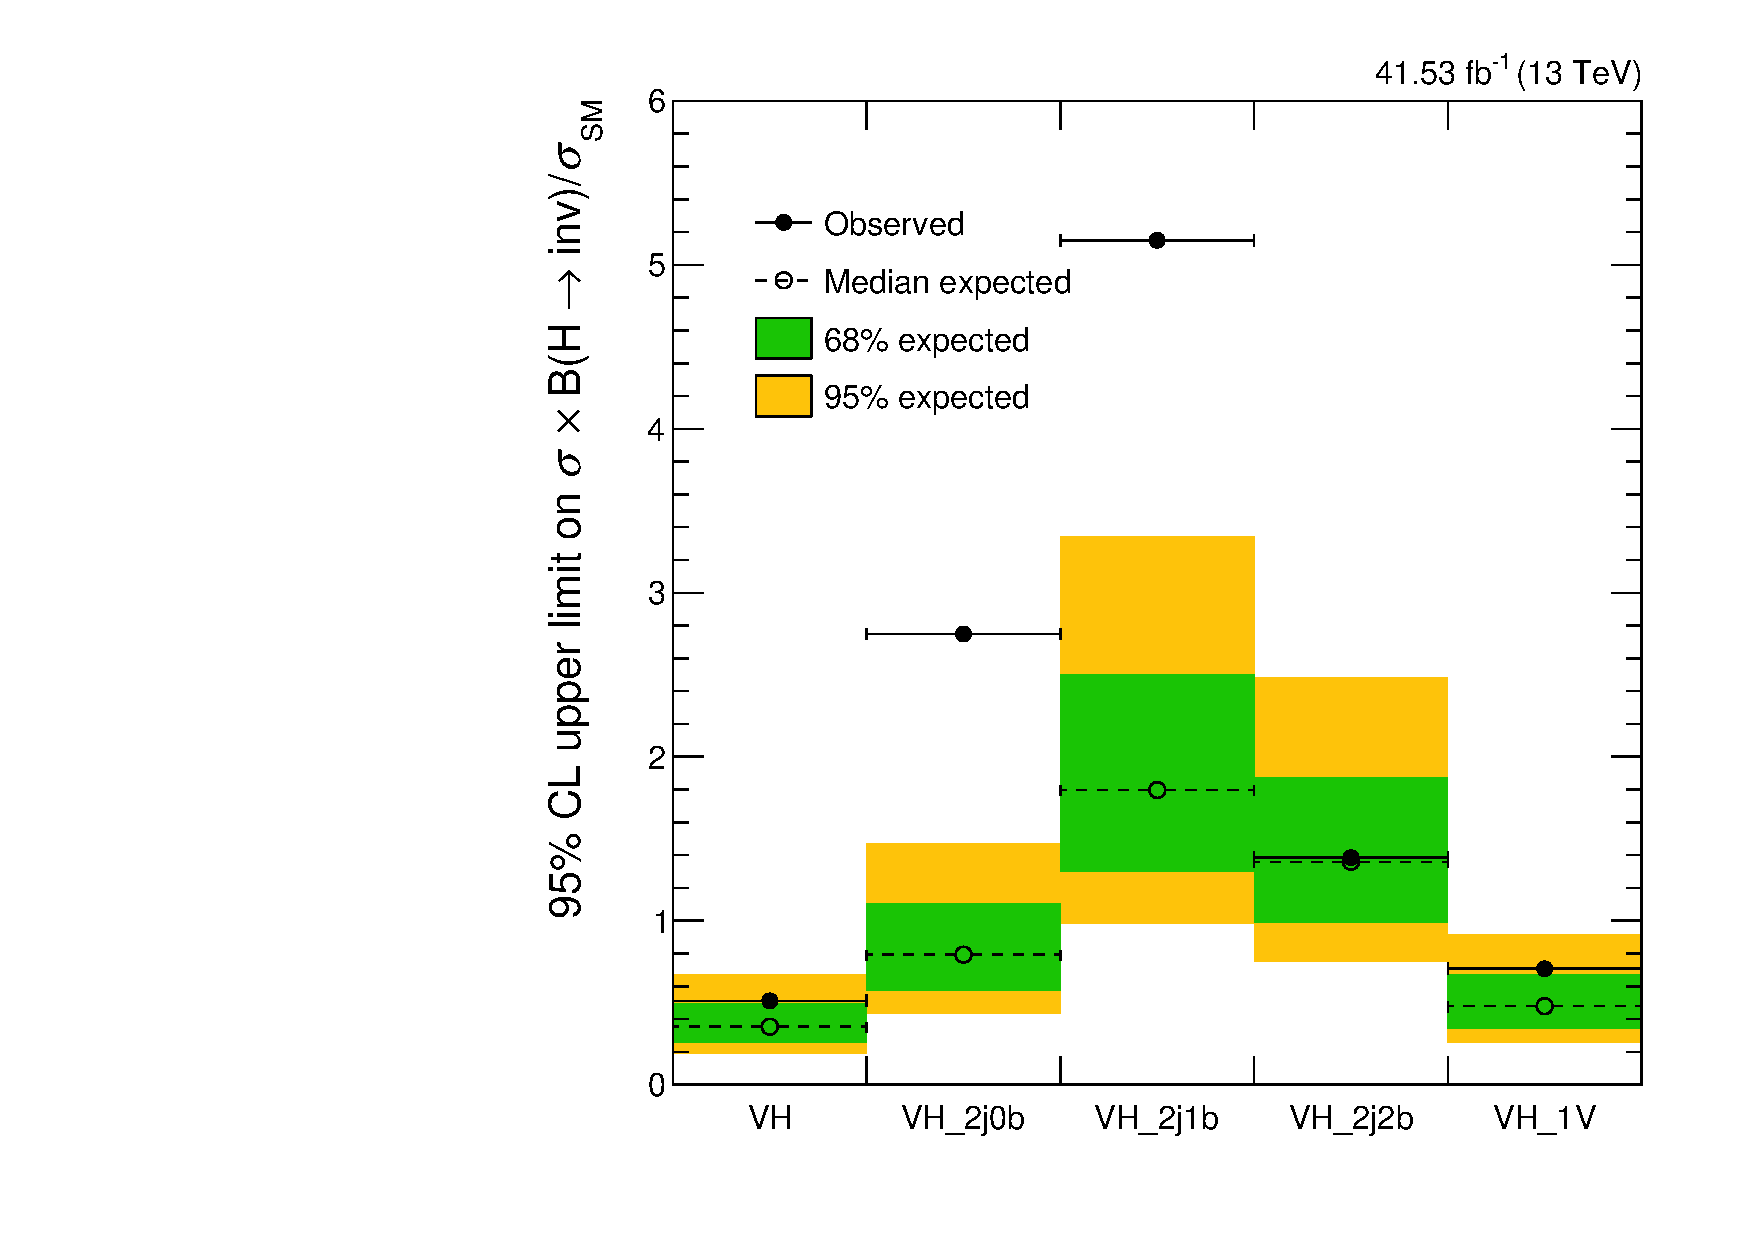
\includegraphics[width=\textwidth]{chapters/higgstoinv/figures/limits/VH/limit_2017_VH.pdf}
        \caption{\VH --- 2017}
    \end{subfigure}

    \begin{subfigure}[b]{0.45\textwidth}
        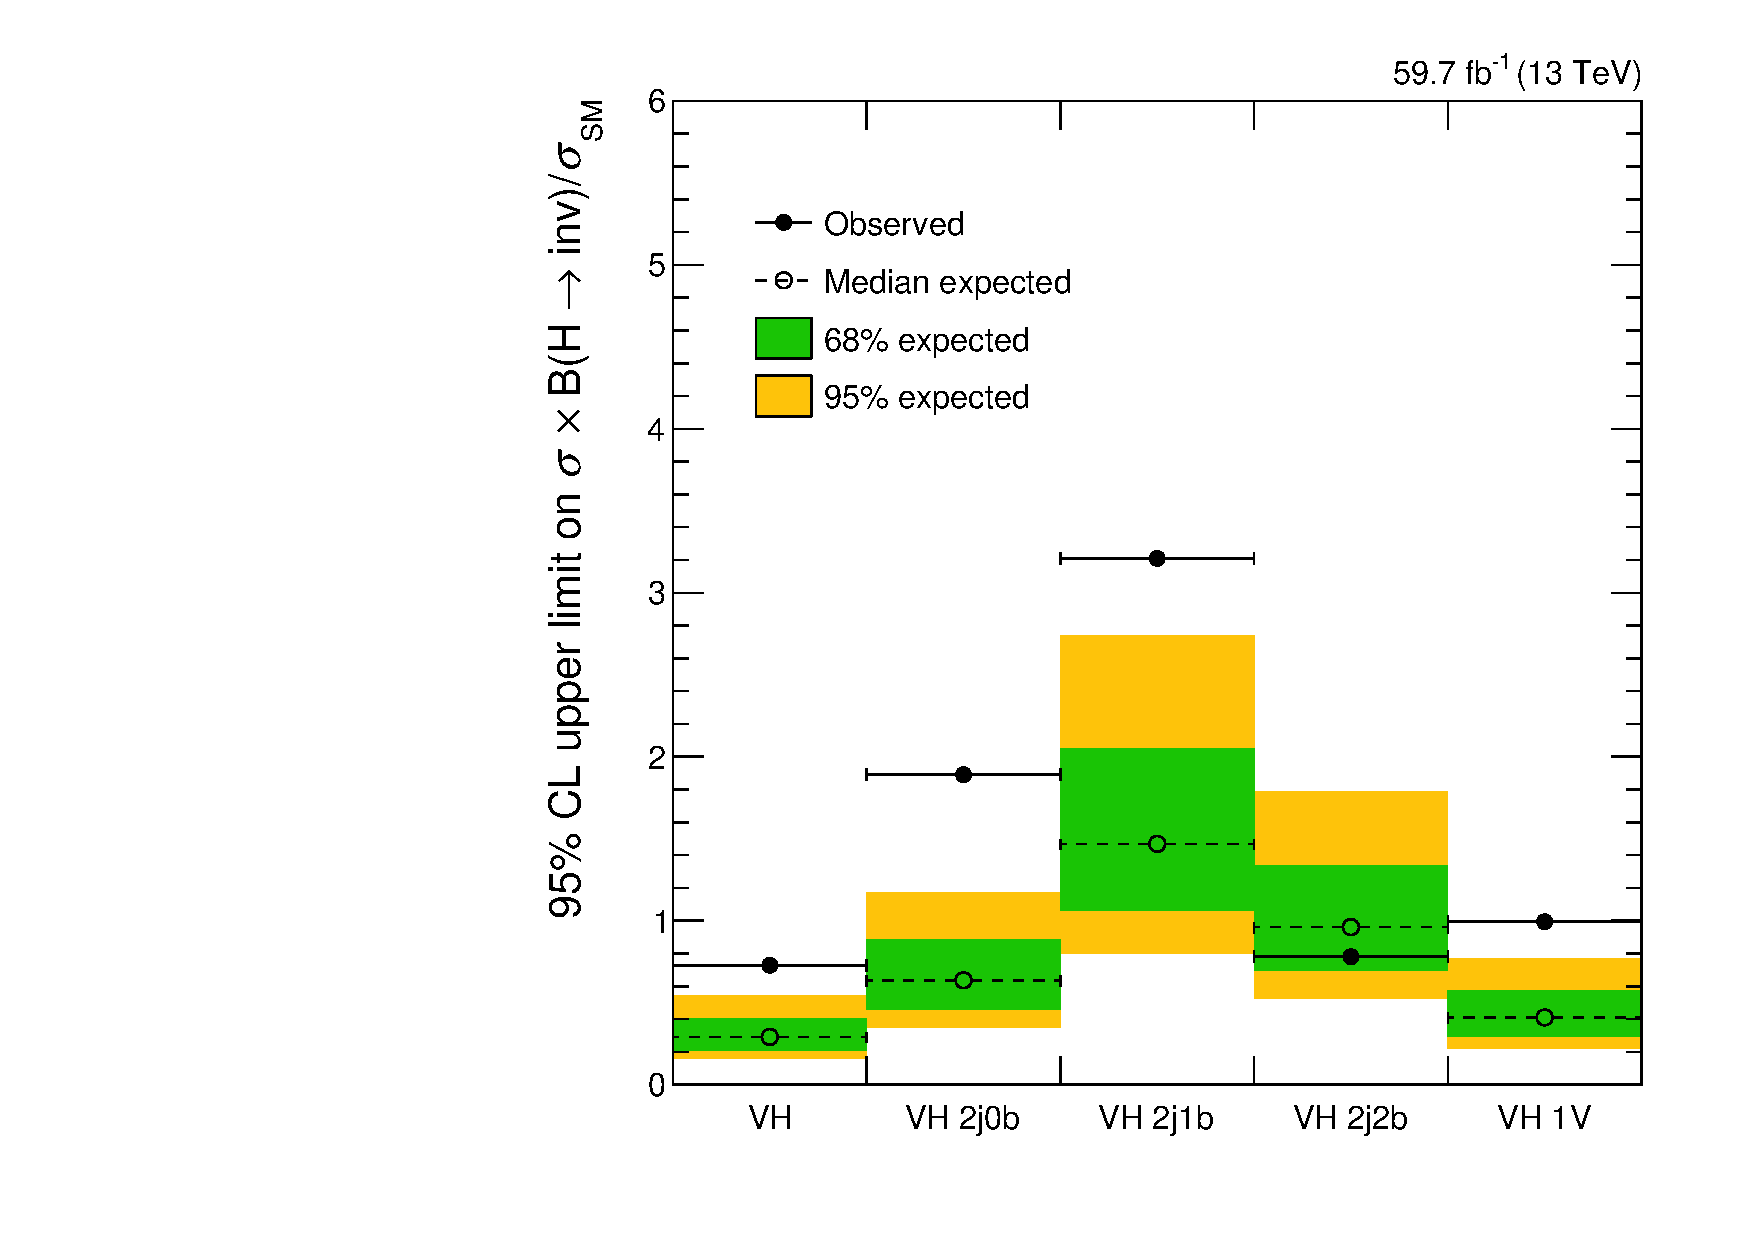
\includegraphics[width=\textwidth]{chapters/higgstoinv/figures/limits/VH/limit_2018_VH.pdf}
        \caption{\VH --- 2018}
    \end{subfigure}
    \caption[Observed and expected 95\,\% CL upper limits on the Higgs boson to invisible state branching fraction in the \VH channel, for both the individual categories, and the combination of them, for each data-taking year in Run-2]{Observed and expected 95\,\% CL upper limits on the Higgs boson to invisible state branching fraction in the \VH channel, for both the individual categories, and the combination of them, for each data-taking year in Run-2.}
    \label{fig:htoinv_limit_VH_per_year}
\end{figure}

\begin{figure}[htbp]
    \centering
    \begin{subfigure}[t]{0.45\textwidth}  % top align since figures are same dimensions, but x-axis labels are larger for likelihood
        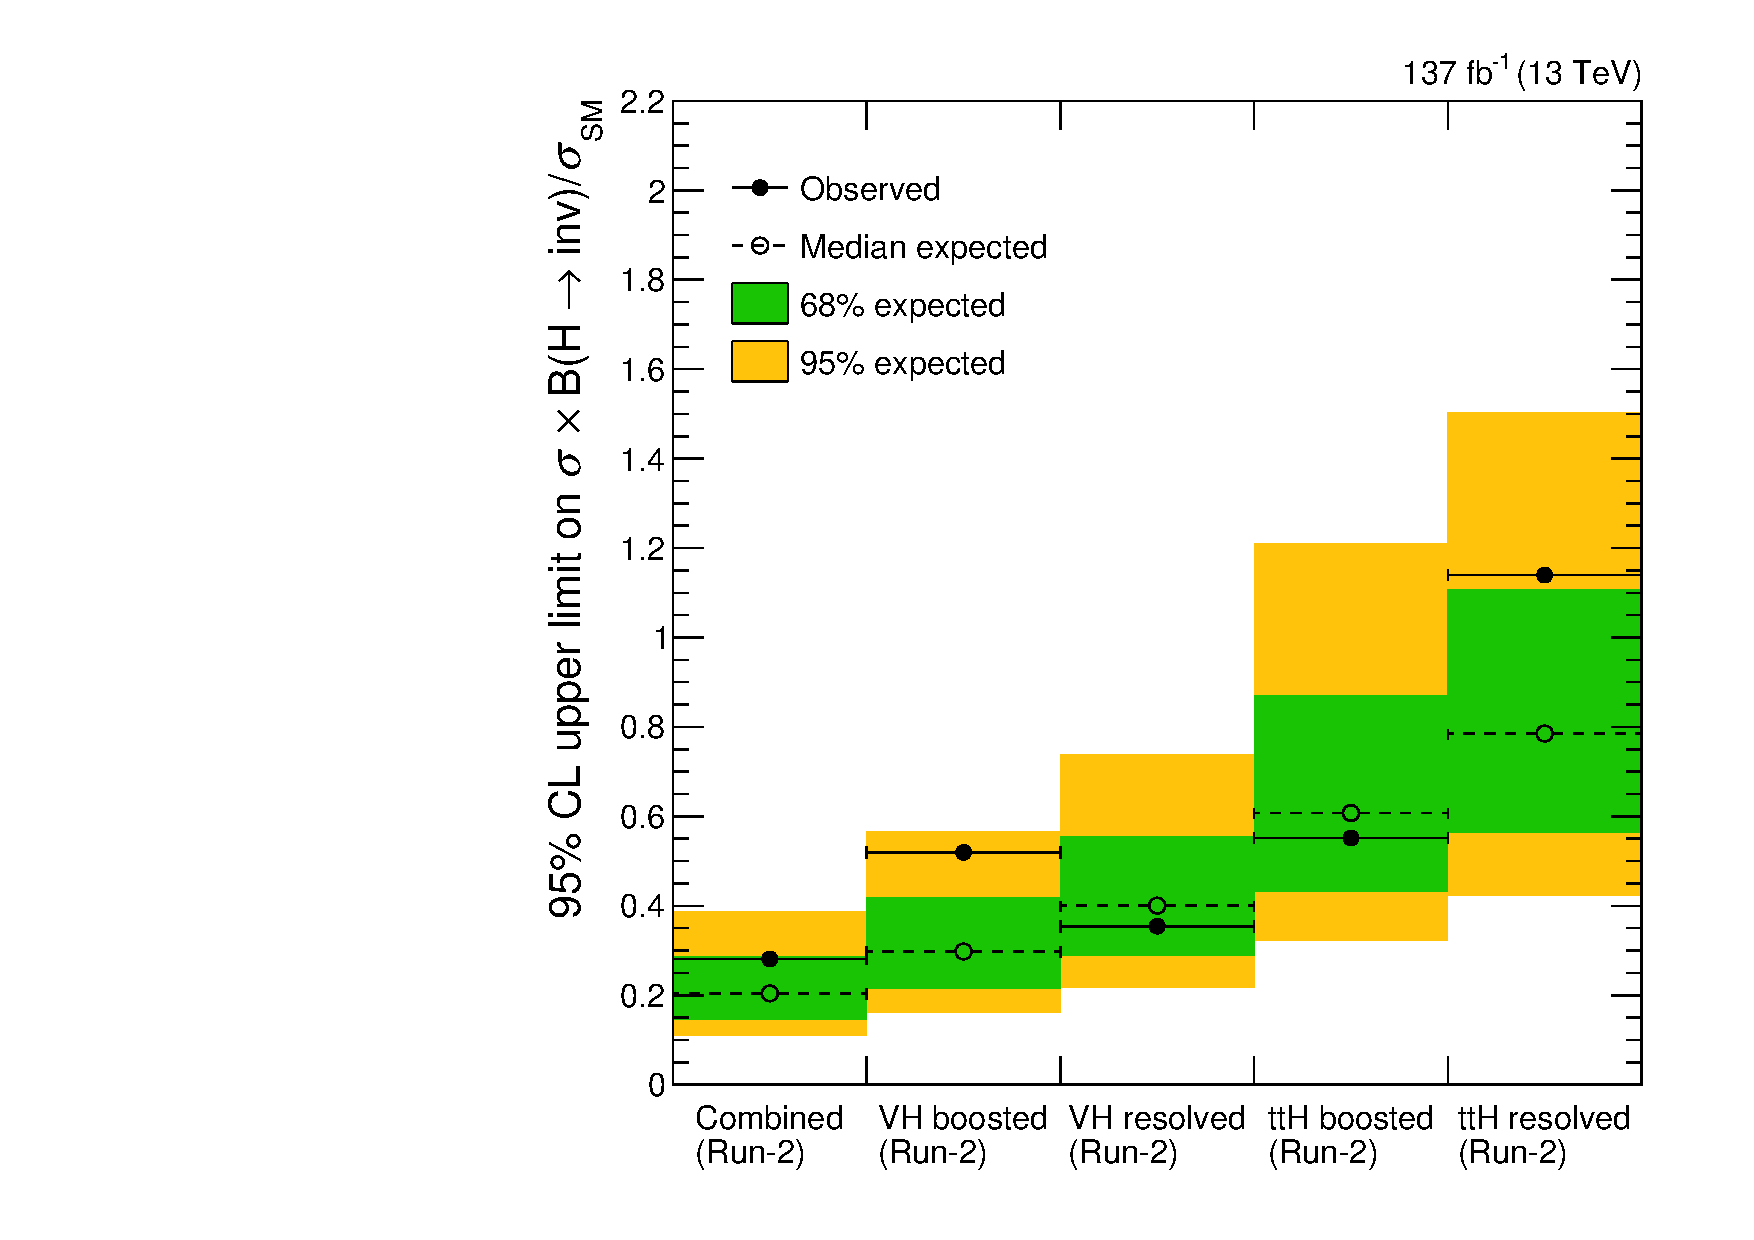
\includegraphics[width=\textwidth]{chapters/higgstoinv/figures/limits/full_Run2/limit_Run2_ttH_VH_resolved_boosted.pdf}
        \caption{Limit --- Run-2}
    \end{subfigure}
    \hspace{0.05\textwidth}
    \begin{subfigure}[t]{0.45\textwidth}
        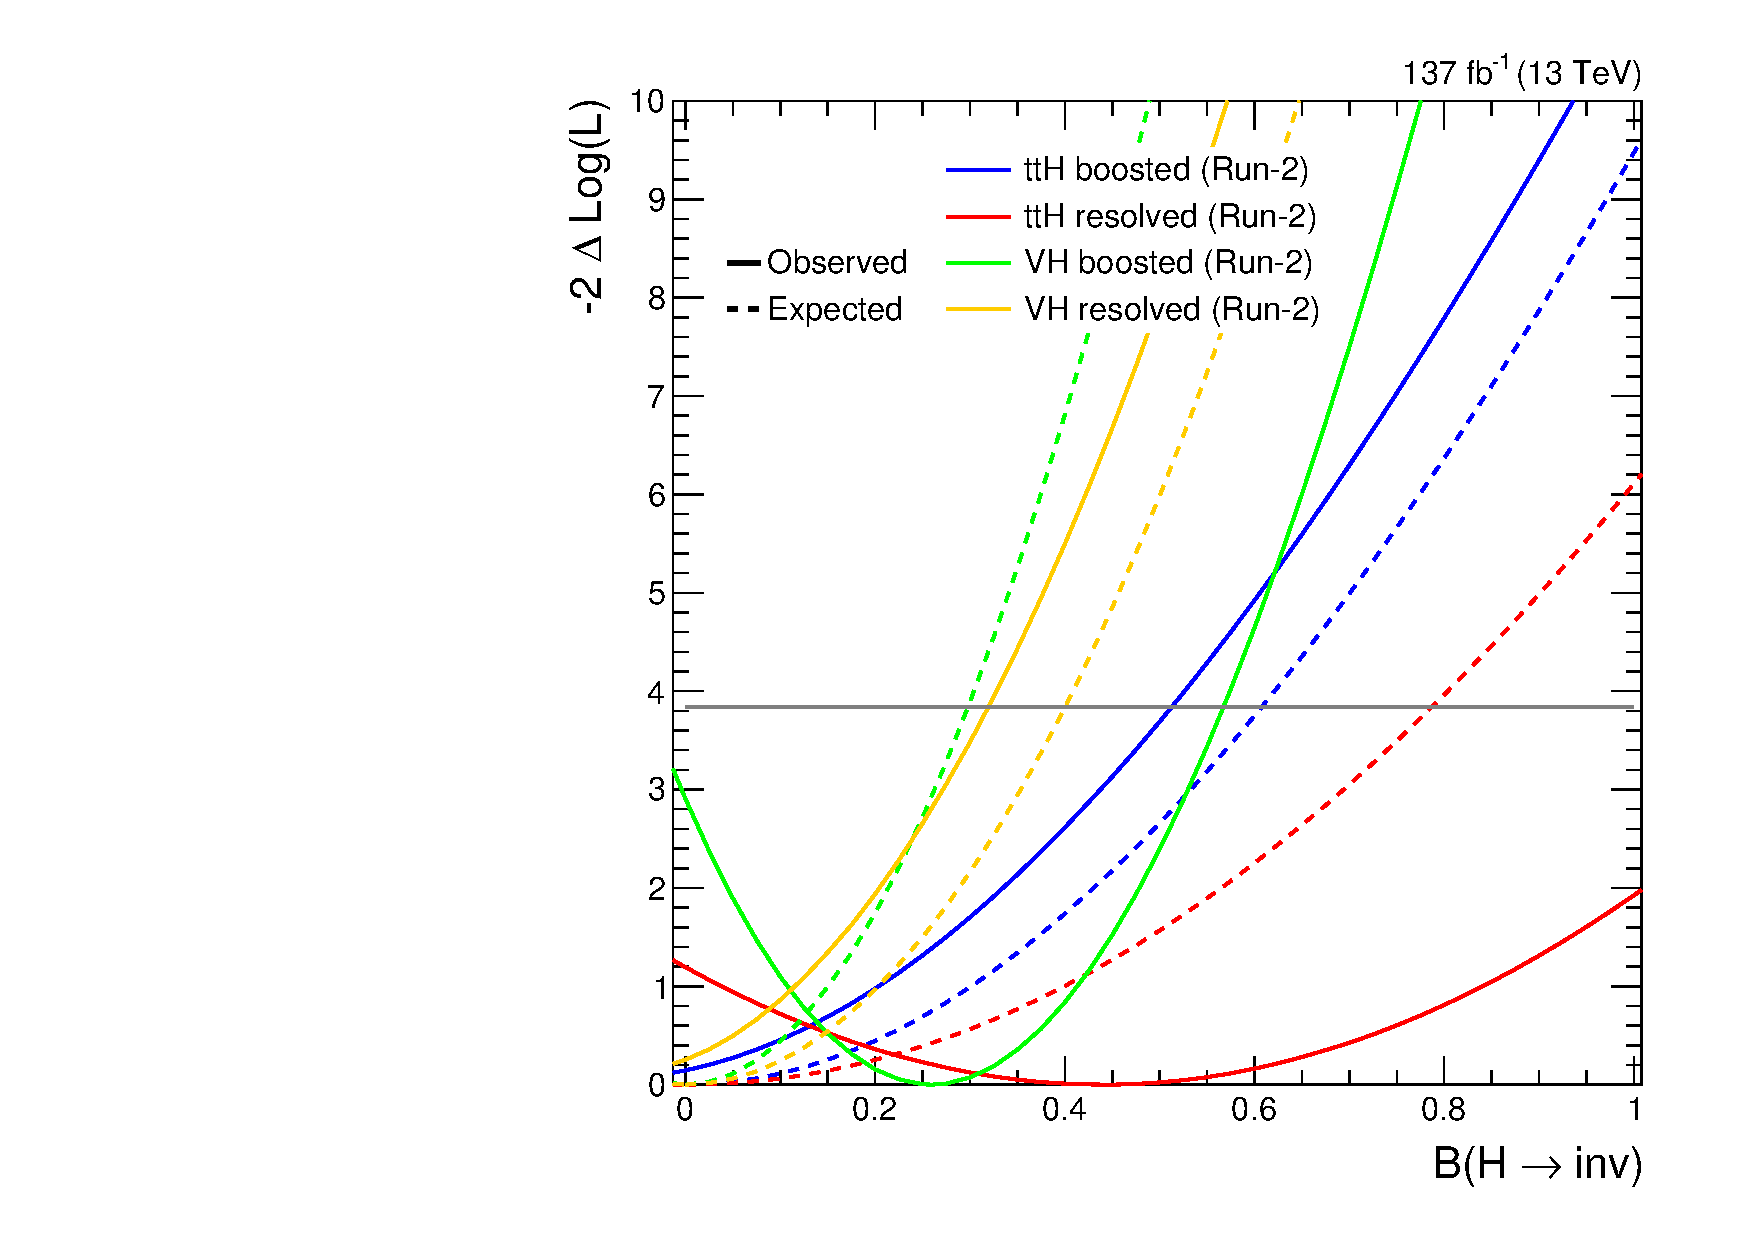
\includegraphics[width=\textwidth]{chapters/higgstoinv/figures/likelihood_scan/profile_likelihood_scan_Run2_ttH_VH_resolved_boosted.pdf}
        \caption{Profile likelihood --- Run-2}
    \end{subfigure}
    \caption[Observed and expected 95\,\% CL upper limit on the Higgs boson to invisible state branching fraction $\BRof{\higgstoinv}$ and the corresponding profile likelihood scan, in the \ttH and \VH boosted and resolved category groupings and their combination, for the full Run-2 dataset]{Observed and expected 95\,\% CL upper limit on the Higgs boson to invisible state branching fraction $\BRof{\higgstoinv}$ (left) and the corresponding profile likelihood scan (right), in the \ttH and \VH boosted and resolved category groupings and their combination, for the full Run-2 dataset.}
    \label{fig:htoinv_limit_likelihood_boosted_resolved_cats_Run2}
\end{figure}
